\documentclass[12pt]{report}
\usepackage[utf8]{inputenc}
\usepackage[style=apa,sortcites=true,sorting=nyt,backend=biber]{biblatex}
\addbibresource{EBC.bib}
\usepackage[
            colorlinks=true,        
            allcolors = black,  
            citecolor=blue,        
        ]{hyperref}
\AtEveryCite{\color{blue}}       

\usepackage{graphicx}
\graphicspath{ {images/} }
\usepackage{graphicx} % Required for inserting images
\usepackage[titles]{tocloft}
\usepackage{sectsty}
\usepackage{amsmath}
\usepackage{mathtools}
\usepackage{amssymb}
\usepackage{stmaryrd}
\usepackage{comment}
\usepackage{dsfont}
\usepackage{algorithm}
\usepackage{algpseudocode}
\usepackage{caption}
\linespread{1.5}




\def\cred{\color{red}}
\def\cblue{\color{blue}}
\newtheorem{remark}{Remark}[section]
\newtheorem{exam}{\textsc{Example}}[section]
\newtheorem{theorem}{Theorem}[subsection]
\newtheorem{proposition}{Proposition}[section]
\newtheorem{lemma}{Lemma}[subsection]
\newtheorem{algorithmold}{Algorithm}[section]
\newtheorem{definition}{Definition}[subsection]
\newcommand{\1}{\mathbf{1}}
%\newcommand{\1}{\mathds{1}}
\def\be{\begin{equation}}
\def\ee{\end{equation}}

\usepackage[a4paper, portrait, margin=0.9in]{geometry}

\sectionfont{\LARGE}
\subsectionfont{\Large}
\subsubsectionfont{\large}

\setcounter{tocdepth}{4}
\setcounter{secnumdepth}{4}

\begin{document}

\begin{titlepage}
   \begin{center}
       \vspace*{1cm}
        \LARGE
       \textbf{Modelling Tail Risk with Empirical Copulas} \\

       \vspace{2cm}
        \LARGE
       \textbf{Tong Pun Yat}

       
        
       \vspace{7.0cm}
       \Large
       STAT4798 Statistics and Actuarial Science Project
            
       \vspace{0.8cm}
            
       Department of Statistics and Actuarial Science\\
       The University of Hong Kong\\
       30 April 2024
            
   \end{center}

\end{titlepage}

\newpage
\begin{flushleft}
\LARGE
\textbf{Abstract} \\
\normalsize
\vspace{1cm}
The empirical copula is a nonparametric method to model dependence, without the need of pre-specifying marginal distributions. Over the years, various statisticians have proposed new variations of the empirical copula, such as the empirical beta copula, empirical checkerboard copula, and most recently, the data-adaptive empirical copulas. Assessing tail risk with such copulas often leads to underestimation, due to the lack of available data beyond the largest / smallest observation which leads to difficulties in fitting the upper and lower tail accurately. This report provides an oversight on how well empirical copulas can fit the upper and lower tail, by computing the exceedance and cumulative probabilities, and comparing the estimated probabilities with the corresponding true copula. It is found that the data-adaptive empirical copulas proposed by \cite{KojadinovicYi2024Smooth} exhibits the best performance despite some erratic patterns and systematic underestimation. The low-Kendall's-tau region is also heavily affected by the limited sample size.
\end{flushleft}

\newpage
\begin{flushleft}
\LARGE
\textbf{Preface} \\
\normalsize
\vspace{1cm}
Prof. Hofert has provided inspiration and motivation behind this project (understanding the overestimation and underestimation of tail risk). I have developed the algorithm in its entirety, reviewed by Prof. Hofert, where he has given comments on how to improve the simulation. The report is also typed entirely by me, where the first half of the report are prerequisites, which are in reference with various relevant publications (most notably \cite{HofertBook}, \cite{KojadinovicYi2024Smooth}, \cite{SegersEBC}); and the second half of the report is original, with parts of the R code referencing \cite{copulaRPackage2023}, \cite{KojadinovicYi2024Smooth} with some modifications from me. 
\end{flushleft}

\newpage
\begin{flushleft}
\LARGE
\textbf{Acknowledgements} \\
\normalsize
\vspace{1cm}
I would like to thank Prof. Hofert, my supervisor for STAT4798, for his continued guidance in the entirety of this project, where he has introduced the underlying motivation around this topic and on copulas overall. I would also like to especially thank my friend Yao Hui for assisting in running the (super long) R algorithm for me (as my computer did not have sufficient memory / RAM to handle the simulation). I would also like to thank my friends for their continued support during this course, and lastly my girlfriend Tiffannie, or I wouldn't have stood till now.
\end{flushleft}

\tableofcontents
\renewcommand\thesection{\arabic{section}}

\newpage
\begin{flushleft}
\sectionfont{\fontsize{20}{15}\selectfont}
\subsectionfont{\fontsize{17}{15}\selectfont}
\section{Introduction}
\vspace{0.5cm}
\subsection{Motivation}
\vspace{0.5cm}
\normalsize
In introductory statistics, we borne the need to understand the relationship between multiple underlying variables to make statistical inference. By analysing them in a univariate way, we gain intuition on the distributional characteristics of the marginal distributions, while multivariate analysis allow us to understand the dependence between variables. To begin with, we can start with linear dependence. Notably, we generalise the linear relationship between variables with correlation coefficients: \\
\vspace{0.5cm}
\begin{align*}
\rho = \begin{pmatrix} 
    1 & \rho_{12} & \dots & \rho_{1d} \\
    \rho_{21} & 1 & \dots & \rho_{2d} \\
    \vdots & \vdots & \ddots & \vdots \\
    \rho_{n1} & \rho_{n2} & \dots & 1
\end{pmatrix}
, \: \rho_{ij} = \frac{Cov(X_{i},X_{j})}{\sqrt{Var(X_{i})Var(X_{j})}}
\end{align*} \\
\vspace{0.5cm}
However, we realise that this metric is only useful when evaluating linear relationships between variables (or transformed variables). A low correlation coefficient does not imply a weak relationship as variables might exhibit non-linear dependence. \\
\vspace{0.5cm}
Copulas, as investigated in this report, can describe the dependence between the components of the random vectors. However in reality, while dealing with messy datasets, it is challenging to infer the unknown copula and marginal distributions by observation. Parametric or semiparametric methods of estimating the copula are often biased as the parametric family of copulas have to be specified beforehand, which is often unrealistic. A possible workaround of this problem is to utilise nonparametric estimation of copulas, which does not require prior knowledge on the family of copulas when undergoing statistical inference. \\
\vspace{0.5cm}
Empirical copulas, first proposed by \cite{DeheuvelsEC}, analyse the multi-dimensional pseudo-observations (estimated nonparametrically as the ranks of the components of the random vector) componentwise, and can be shown to have a similar shape to the real estimated copula. However, tbhe classical empirical copula is not a copula itself as it has discrete uniform margins instead of continous ones. \\
\vspace{0.5cm}
To overcome this shortcoming, multiple smoothed copulas built on the basis of empirical copulas are proposed. They include a multilinear extension of the empirical copula, the empirical checkerboard copula (as defined by \cite{CarleyTaylorECC} and \cite{HofertBook}), the empirical beta copula \parencite{SegersEBC}, and recently, generalised smooth copula estimators (that contain the empirical beta copula) proposed by \cite{KojadinovicYi2024Smooth}. \\
\vspace{0.5cm}
In present time, tail risk is still little understood and often underestimated. It is known that the usage of the no-tail-dependent Gaussian copula in the modelling of default probability of securities (and tranches) with mortgage underlyings have indirectly led to the financial crisis in 2007, where securities were mispriced due to the underestimation of tail default risk. The usage of the wordings ``1-in-500" in describing the massive flood that happened in Hong Kong during late 2023 is widely misunderstood, as there are no 500-year worth of data in understanding an event of this scale. Yet, due to global warming, these large scale national disasters will be recurring (or even commonplace) in the near future, which brings the urgency in developing tail risk modelling techniques. \\
\vspace{0.5cm}
In this report, we try to understand whether the class of empirical copulas systematically underestimates tail risk with respect to the true underlying copula by computing the up-tail and low-tail probability of the class of empirical copulas and compare it to the true up-tail and low-tail probability. This could extend the possibility that even for a small sample size empirical copulas can be more widely applied in the modelling of tail risks without the risk of misspecifying the class of copulas and with added accuracy compared to other parametric / semiparametric methods. \\
\vspace{0.5cm}

\newpage

\section{Prerequisites: Copulas}
\vspace{0.5cm}
\subsection{Definition and Construction}
\vspace{0.5cm}

We first establish two important (and well-known) results on probability transformation. When $F$ is a continuous distribution, $F^{-1}$ is equivalent to the inverse of $F$.\\


\begin{lemma}\label{IntegralTransform} 
\textbf{Integral Transform} \\

For a r.v. $X$ $\sim$ $F$ where $F$ is a continuous distribution function $\Rightarrow$ $F(X)$ $\sim$ $\mathcal{U}(0,1)$.
\end{lemma}
Proof:  \parencite{HofertBook} $F_{F_{X}}(x)$ = $P(F_{X}(x) $$\le$ $y$) = $P(X \le F^{-1}_{X}(y))$ = $F_{X}(F^{-1}_{X}(y))$ = $y \Rightarrow F(X)$ $\sim$ $\mathcal{U}(0,1)$ 
\\


\begin{lemma}\label{QuantileTransform}
\textbf{Quantile Transform} \\

For a r.v. $U \sim \mathcal{U}(0,1)$, $F$ and $F^{-1}$ being any distribution function and its corresponding quantile function respectively $\Rightarrow$ $F^{-1}_{X}(U) \sim F $.
\end{lemma}
Proof: Similar to \textbf{Lemma 1.1}, $P(F^{-1}_{X}(U) \le x) = P(U \le F_{X}(x)) = F_{X}(x)$
\\

\vspace{0.5cm}
These two transformation implies that it is trivial to transform any continuous distribution into a standard uniform distribution, and subsequently to another continuous distribution of interest. This allows us to relate random variables with different underlying distributions easily. We can generalise dependence by creating a continuous multivariate distribution function that links all the marginal standard uniform distributions. 

\vspace{0.5cm}
The definition of Copula is illustrated below, with reference to \cite{HofertBook}.\\

\begin{definition}\label{CopProperties}
\textbf{Copula} \\
A copula is a continuous d-dimensional distribution function $C(u_{1}, u_{2}, \dots, u_{d}) $ that satisfies the following properties: \\
\begin{enumerate}
    \item Groundedness: \: $C(u_{1}, \dots, u_{i-1}, 0, u_{i+1}, \dots, u_{d}) = 0$ if any $u_{i} = 0$.\\
    \item $\mathcal{U}(0,1)$ margins: \: $\forall i \in \{1, \dots,d\}, \: C(1, \dots, 1, u_{i}, 1, \dots, 1) = u_{i}$\\
    \item d-increasing: $\: \textbf{a}, \textbf{b} \in [0,1]^{d}, \Delta_{(\textbf{a},\textbf{b}]}C = \sum\limits_{i \in \{0,1\}^{d}} (-1)^{\sum_{j=1}^{d}i_{j}}C(a_{1}^{i_{1}}b_{1}^{1-i_{1}}, \dots, a_{d}^{i_{d}}b_{d}^{1-i_{d}})  \ge 0 $, \: where $\Delta_{(\textbf{a},\textbf{b}]}C$ is the C-volume defined w.r.t hyperrectangle $(\textbf{a},\textbf{b}]$.
\end{enumerate}
\end{definition}


% cite sklar
What makes copulas so popular is its uniqueness under a continuous framework. This is brought about by the famous results of Sklar's Theorem.

\begin{theorem}\label{SklarTheorem}
\textit{\normalfont \parencite{SklarTheorem}}
\textbf{Sklar's Theorem}
\vspace{-0.2cm}
\begin{enumerate}
    \item Existence: For univariate margins $F_{1}, F_{2}, \dots, F_{d} \sim \mathcal{U}(0,1)$, a d-dimensional distribution function $F$, $\exists C: [0,1]^{d} \rightarrow [0,1]$ such that $F(\textbf{x}) = C(F_{1}(x_{1}), \dots, F_{d}(x_{d}))$, $\textbf{x} \in \mathbb{R}^{d}$, where $C$ is uniquely defined on $\prod_{j=1}^{d} ran \: F_{j}$.
    \item Converse: Given any copula $C: [0,1]^{d} \rightarrow [0,1]$ and univariate margins $F_{1}, F_{2}, \dots, F_{d}$, $F(\textbf{x}) = C(F_{1}(x_{1}), \dots, F_{d}(x_{d}))$ is a d-dimensional distribution function, $\textbf{x} \in \mathbb{R}^{d}$.
\end{enumerate}
\end{theorem}
Notice that if the univariate margins $F_{1}, F_{2}, \dots, F_{d}$ are continuous (and $\mathcal{U}(0,1)$ distributed), $C$ is uniquely defined. \\
\vspace{0.5cm}
This shows that there is a one-to-one correspondence between the univariate margins to the observable d-dimensional distribution function, linked by a unique copula function. \\
\vspace{0.5cm}

Its' significance can be illustrated by the following analogy provided in \cite{HofertBook}. Consider two d-dimensional random vectors $\textbf{X}$  and $\textbf{Y}$, where its components (marginals) (i.e. $(X_{1}, \dots, X_{d})$ and $(Y_{1}, \dots, Y_{d})$) are distributed differently (e.g. let's propose that $X_{1}, \dots, X_{i}$ are gamma distributed, $X_{i+1}, \dots, X_{d}$ are normally distributed; $Y_{1}, \dots, Y_{i}$ are beta distributed, $Y_{i+1}, \dots, Y_{d}$ are pareto distributed). However, it is unrealistic to compare their dependence as their marginal distribution are different. However, utilising \ref{IntegralTransform} can allow us to transform all marginal distributions to standard uniform margins, then applying a Copula function to model dependence. If it is provided that the random vectors are continuous, Having the same joint distribution (or the same copulas) implies that they have the same dependence structure.\\
\vspace{0.5cm}
It's ability to model dependence between multivariate vectors can be amplified by the invariance principle. The theorem presented below is obtained from \cite{HofertBook}: \\

\newpage
\begin{theorem}\label{CopulaInvariance}
\textbf{Invariance Property of Copulas} \\

Let $\textbf{X} \sim F$ with continuous univariate margins $F_{1}, F_{2}, \dots, F_{d}$ and copula $C$. It follows that $T_{1}(X_{1}), T_{2}(X_{2}), \dots, T_{d}(X_{d})$ also has copula $C$, where $\forall j \in $\{$1$, \dots, $d$\}, $T_{j}$ is a strictly increasing function on ran $X_{j}$. 
\end{theorem}

Proof:
\begin{align*}
\Rightarrow P(T_{1}(X_{1}) \le x_{1}, \dots, T_{d}(X_{d}) \le x_{d}) &= P(X_{1} \le T_{1}^{-1}(x_{1}), \dots, X_{d} \le T_{d}^{-1}(x_{d})).\\
&= C(F_{1}(T^{-1}_{1}(x_{1})),F_{2}(T^{-1}_{2}(x_{2})), \dots, F_{d}(T^{-1}_{d}(x_{d})))
\end{align*}

We can also see that $\forall j \in $\{$1$, \dots, $d$\}, $P(T_{j}(X_{j}) \le x_{j})$ = $P(X_{j} \le T_{j}^{-1}(x_{j}))$ = $F_{j}(T^{-1}_{j}(x_{j}))$
and the result follows.

\vspace{0.5cm}

Copulas can provide a way to understand the dependence without knowledge of the original (before-transformed) marginal distribution, and the fact that imposing an increasing transformation does not distort dependence allows flexibility in transforming the variable to standard uniform marginals without the worry of over or underestimating dependence. \\

\vspace{0.5cm}

Before introducing some common copula families and distributions, it is best to define a bound for the possible values of a copula. The definitions are obtained from \cite{HofertBook}. \\ 

\begin{theorem}\label{FrechetHoeffdingBound}
\textit{\normalfont (\cite{höffding1940maßstabinvariante}; \cite{FrechetBounds})}
\:\textbf{Frech\'et-Hoeffding Bounds} \\
\vspace{-0.8cm}
\begin{align*}
C^{-}(\textbf{u}) = \max \{ \sum_{j = 1}^{d} u_{j} - d + 1, 0 \}, \:
C^{+}(\textbf{u}) = \min_{1 \le j \le d} \{u_{j}\}
, \: \textbf{u} \in [0, 1]^d \\
\end{align*}
\vspace{-2.5cm}
\begin{align*}
\Rightarrow \forall \: C(\textbf{u}), \: C^{-}(\textbf{u}) \le C(\textbf{u}) \le C^{+}(\textbf{u}), \: \textbf{u} \in [0, 1]^d
\end{align*}
\end{theorem}

This establishes the maximal and minimal value of a copula (which is analogically similar to +1 and -1 in pearson's correlation coefficient). Note that $C^{-}(\textbf{u})$ at d = 2 is the countermonotonic copula and $C^{+}(\textbf{u})$ is the comonotonic copula.\\

% these definition from marius's book

\newpage
\subsection{Common Copula distributions}
\vspace{0.5cm}
Distributions of Copulas have been well-researched in the past decade. There are three main copula classes: Archimedean copulas, Elliptical copulas and Extreme-value copulas. In this report, we focus on the first two classes. Definition of these copulas are obtained from \cite{HofertBook}.
\subsubsection{Archimedean Copulas}
\vspace{0.5cm}

\begin{definition}\label{ArchimedeanDefinition}
\textit{\normalfont\parencite{HofertBook}} \:\textbf{Archimedean copula} \\

C(\textbf{u}) is an archimedean copula if it exhibits the following form: \\
\vspace{-0.8cm}
\begin{align*}
C(\textbf{u}) = \psi(\psi^{-1}(u_{1}) + \psi^{-1}(u_{2}) + \dots + \psi^{-1}(u_{d})), \: \textbf{u} \in [0, 1]^d
\end{align*}
where $\psi$ is a generator function.
\end{definition}

\begin{definition}\label{GeneratorDefinition}
\textit{\normalfont\parencite{HofertBook}} \:\textbf{Generator Function} \\

$\psi$ is a generator function for an archimedean copula if it exhibits the following properties: \\
\begin{enumerate}
\item $\psi : [0,\infty] \rightarrow [0,1]$ is continuous, strictly decreasing; $\psi(0) = 1$, $\psi(\infty) -> 0$
\item $\psi \in \Psi$, where $\Psi$ is the class of all generators
\item $ \forall k \in \{0, \dots, d - 2 \}, (-1)^{k} \psi^{(k)}(t) \ge 0$ and $(-1)^{d-2}\psi^{(d-2)}(t)$ is nonincreasing and convex on $t \in (0,\infty)$ \normalfont{(d-monotonicity)}
\end{enumerate}
\end{definition}
Note that if $\forall k \in \{0, \dots, d \}, (-1)^{k} \psi^{(k)}(t) \ge 0$, $\psi$ is completely monotone. \\

For the purpose of this report, only heavy-tailed copulas are presented below:\\
\begin{enumerate}
\item \textbf{Clayton copula} \parencite{ClaytonCopula} \\
\vspace{0.5cm}
$C^{C}_{\theta}(\textbf{u})$ = $\left\{
\begin{array}{ll} 
\max \{ u_{1}^{-\theta} + u_{2}^{-\theta} - 1, 0 \}^{-1/\theta}, \: \: d = 2, \: \theta \in [-1,\infty) \backslash \{ 0 \}, \: \textbf{u} \in [0,1]^{2} \\
(1 - d + \sum_{j = 1}^{d} u^{- \theta}_{j} )^{-1/\theta}, \: \: d \ge 3, \; \theta \in (0,\infty), \: \textbf{u} \in [0,1]^{d}
\end{array} 
\right.$ 
\\
\vspace{0.5cm}
where $\psi(t)$ = $(1 + t)^{-1/\theta}$ 

\newpage
\item \textbf{Gumbel-Hougaard copula} (\cite{GumbelCopula}; \cite{HougaardCopula}) \\ 

\vspace{0.5cm}
$C^{GH}_{\theta}(\textbf{u})$ = $\exp \left( -( \sum\limits_{j = 1}^{d} (- \ln u_{j})^{\theta})^{1/\theta} \right)$, $\theta \in [1,\infty) $, $\textbf{u} \in [0,1]^{d}$ 
\\
\vspace{0.5cm}
where $\psi(t)$ = $\exp(-t^{1/\theta})$
\end{enumerate}

It is noted that Clayton copulas have unusually high weight on the left (low) tail, and Gumbel-Hougaard have unusually high weight on the right (upper) tail, hence these copulas are used to evaluate the effectiveness of evaluating low and upper tail risk by the class of empirical copulas. \\

\subsubsection{Elliptical Copulas}
\vspace{0.5cm}

\begin{definition}\label{EllipticalDefinition}
\textit{\normalfont\parencite{HofertBook}} \:\textbf{Elliptical copula} \\

C(\textbf{u}) is an elliptical copula if it exhibits the following form: \\
\vspace{-0.8cm}
\begin{align*}
C(\textbf{u}) = H(F^{-1}_{1}(u_{1}), \dots, F^{-1}_{d}(u_{d})), \: \textbf{u} \in \prod\limits_{j=1}^{d} ran F_{j}
\end{align*}
where $H$ is a multivariate elliptical distribution function, $F_{1}, \dots, F_{d}$ are the univariate margins.
\end{definition}

\begin{definition}\label{EllipticalDistribution}
\textit{\normalfont\parencite{HofertBook}}
\:\textbf{Elliptical distribution} \\

\textbf{X} is an elliptical distribution if it exhibits the following form: \\
\vspace{-0.8cm}
\begin{align*}
\textbf{X} = \boldsymbol{\mu} + R\textbf{A}\textbf{S}
\end{align*}

where $\textbf{S} \sim \mathcal{U}( \{ \textbf{x} \in \mathbb{R}^{k} : \|\textbf{x}\| = 1 \} )$ is uniformly distributed across the unit sphere of order k, $\textbf{A}$ is the lower triangular square matrix with nonnegative entries such that $\textbf{A}\textbf{A}^{T}$ = $\sum$, where $\sum$ is the covariance matrix (Cholesky decomposition of $\sum$), and R $\ge$ 0 having a density:
\begin{align*}
f_{R}(r) = \frac{2 \pi^{\frac{d}{2}} r^{d-1} g(r^{2})}{\Gamma(\frac{d}{2})}
\end{align*}
\end{definition}

It is remarked that if rank($\sum$) = d (full rank), then the density function of X exhibits the form: \\

\begin{align*}
h(\textbf{x}) = \frac{1}{\sqrt{det \: \Sigma}} \: g \left( (\textbf{x} - \boldsymbol{\mu})^{T} \Sigma^{-1} (\textbf{x} - \boldsymbol{\mu})  \right)
\end{align*}
where $g : [0,\infty) \rightarrow [0,\infty)$ is the density generator

If we supply a specific $g$, a different elliptical copula can be created. The two main copulas in the elliptical copula class are t copulas and normal copulas. Although only t copulas have heavy tail on both tails, considering the significance of the Gaussian copulas, both copulas are listed below: \\

\begin{enumerate}
\item \textbf{Student t copula} \textit{\normalfont\parencite{HofertBook}} \\

The density generator $g$ exhibits the form:\\
\vspace{0.5cm}
$g(t) = \frac{\Gamma(\frac{v+d}{2})}{(\pi v)^{\frac{d}{2}}\Gamma(\frac{v}{2})} \left( 1+\frac{t}{v} \right) ^{-\frac{v+d}{2}}, \: t \in [0,\infty)$ \\
\vspace{0.5cm}
then the density of the copula is:\\
\vspace{0.5cm}
$ c^{t}(\textbf{u}) = \frac{\Gamma(\frac{v+d}{2})}{\Gamma(\frac{v}{2})\sqrt{\det \: P}} \left( \frac{\Gamma(\frac{v}{2})}{\Gamma(\frac{v+1}{2})} \right)^{d} \frac{ (1 + \frac{\textbf{x}^{T}P^{-1}\textbf{x}}{v})^{-\frac{v+d}{2}}}{\prod_{j = 1}^{d} (1 + \frac{x_{j}^{2}}{v})^{-\frac{v+1}{2}}} , \: \textbf{u} \in (0,1)^{d}$ \\
\vspace{0.5cm}
where $\textbf{x} = (t^{-1}_{v}(u_{1}), \dots, t^{-1}_{v}(u_{d}))$.\\

\item \textbf{Gaussian copula} \parencite{HofertBook} \\ 
\vspace{0.5cm}

The density generator $g$ exhibits the form:\\
\vspace{0.5cm}
$g(t) = \frac{\exp(-\frac{t}{2})}{(2\pi)^{\frac{d}{2}}}, \: t \in [0,\infty)$ \\
\vspace{0.5cm}
then the density of the copula is:\\
\vspace{0.5cm}
$ c^{n}(\textbf{u}) = \frac{1}{\sqrt{\det \: P}} \exp \left(-\frac{1}{2}\textbf{x}^{T}(P^{-1}-I_{d})\textbf{x} \right), \: \textbf{u} \in (0,1)^{d}$ \\
\vspace{0.5cm}

where $\textbf{x} = (\Phi^{-1}(u_{1}), \dots, \Phi^{-1}(u_{d}))$.\\

\end{enumerate}

It is noted that Student t copulas have high tail dependence on both sides of the tail, while Gaussian copulas do not have tail dependence on both sides of the tail (truly both sides of the spectrum!).\\

\subsubsection{Extreme-value Copulas}
\vspace{0.5cm}

Extreme value copulas are only slightly mentioned due to the fact that the Gumbel-Hougaard Copula is also a extreme-value copula.\\
\vspace{0.5cm}
Considering the one dimensional case, distributional characteristics in the tail are often underestimated, hence it is optimal to fit a distribution that only considers the maximal value of a set of observations. As discussed in \cite{ModellingExtremalEventsForInsuranceandFinance}, By choosing a suitable block size and obtaining the maxima, it can be seen that, if suitably normalised and let block size n $\rightarrow$ $\infty$, it will converge to the generalised extreme-value distribution.\\
\vspace{0.5cm}
Generalised in multiple literatures (eg. \cite{EVTAnIntro}, \cite{HofertBook}), we can extend this condition to the multivariate case; i.e., if the i.i.d. of block maxima random vectors are suitably normalised, they will converge to the multivariate generalised extreme-value distribution. Note that the marginal distributions are also univariate generalised extreme-value distributions.  \\
\vspace{0.5cm}
The definition of the extreme-value copula are obtained from \cite{HofertBook}.

\begin{definition}\label{ExtremeValueDefinition}
\textit{\normalfont\parencite{HofertBook}} \:\textbf{Extreme-value copula} \\

$C(u)$ is an extreme-value copula if for $\textbf{u} \in [0,1]^{d}$, there exists a $C^{*}$ that exhibits the following properties: 
\begin{align*}
\lim_{n \rightarrow \infty} C^{*}(\textbf{u}^{\frac{1}{n}})^{n} = C(u)
\end{align*}
and $C^{*} \in MDA(G_{\xi})$ (Maximum domain of attraction), where $G_{\xi}$ is the generalised extreme-value distribution with shape parameter $\xi$.
\end{definition}

An important result of extreme-value copulas can be obtained by algebraic manipulation. Proof is omitted but could be found in \cite{HofertBook}.\\

\begin{lemma}\label{MaxStability}
\textit{\normalfont\parencite{HofertBook}} \:\textbf{Max stability characterisation of Extreme-value copulas}\\

A copula $C$ is a extreme-value copula \\
$\iff \forall \textbf{u} \in [0,1]^{d}$ and $r \in \mathbb{N}, \: C(\textbf{u}^{\frac{1}{r}})^{r} = C(\textbf{u})$

\end{lemma}
One notable example of the extreme-value copula is the gumbel-hougaard copula, which is also an archimedean copula.\\

\newpage
\subsection{A Primer in Correlation Measures}
\vspace{0.5cm}
In this section, several rank correlation measures will be introduced as ways to quantify dependence other than the most commonly used pearson's correlation coefficient.

\subsubsection{Pitfalls of Pearson's Correlation Coefficient}
\vspace{0.5cm}
\:\cite{HofertBook} has provided a very detailed analysis on how Pearson's correlation coefficient is deficient in measuring dependence. This report will provide a brief overview on the pitfalls of pearson's correlation coefficient.

\begin{enumerate}
\item \textbf{Nonexistence of correlation coefficient} \\
\vspace{0.5cm}
Recall the definition: $\rho_{ij} = \frac{Cov(X_{i},X_{j})}{\sqrt{Var(X_{i})Var(X_{j})}}$. If either $X_{i}$ or $X_{j}$ does not have a second moment, then $\rho_{ij}$ will be undefined. A possible counterexample is student t distribution with a degree of freedom $v \in (1,2]$, then the second moment is unbounded.
\item \textbf{Invariance property violated} \\
\vspace{0.5cm}
Notice that correlation coefficient measures the magnitude of change of a variable with respect to the opposing variable, hence a linear increasing transformation fulfils the invariance requirement. However, a non-linear transformation (even if increasing) on the random variable will lead to a possible multiplicative / non-linear distortion of the magnitude, which leads to a change in the correlation coefficient as it is only a measure of linear dependence. 
\item \textbf{One-to-one correspondence between marginal distributions and correlation coefficient on the joint distribution violated}\\
\vspace{0.5cm}
A elegant counterexample is provided, originated from stackexchange: \parencite{4665041} \\
$X \in \{-1, 0, 1 \}$, $Y \in \{0, 1\}$, for any $p \in (\frac{1}{6},\frac{1}{3})$,
\begin{align*}
P(X = -1, \: Y = 1) &= P(X = 1, \: Y = 1) = p \\
P(X = -1, \: Y = 0) &= P(X = 1, \: Y = 0) = \frac{1}{3} - p \\
P(X = 0, \: Y = 0) &= 2p - \frac{1}{3} \\
P(X = 0, \: Y = 1) &= \frac{2}{3} - 2p 
\end{align*}
We observe that they have same marginals for all values of $p$, and X and Y are uncorrelated. This shows that there are an infinite amount of joint distributions corresponding to the marginal distribution and correlation.\\
    
\item \textbf{Uncorrelatedness does not imply Independence}\\
\vspace{0.5cm}
A good counterexample would be a transformation on a standard normal random variable:
$X \sim \mathcal{N}(0,1)$. Consider $X^{2}$. $\rho_{X, X^{2}} \neq 0$ but $E[XX^{2}] - E[X]E[X^{2}] = E[X^{3}] - E[X]E[X^{2}] = 0$ as the skewness of a standard normal random variable = 0 due to symmetry.

\item \textbf{Attaining Correlation = --1 or 1 is not necessarily possible for some marginal distributions} \\
\vspace{0.5cm}
A good counterexample would be two Bernoulli random variables. Let $X \sim Ber(p)$, $Y \sim Ber(q)$. By the Frech{\'e}t bounds, the correlation coefficient have the following bounds: \\
\vspace{-0.8cm}
\begin{align*}
\frac{\max(p+q-1,0) - pq}{\sqrt{pq(1-p)(1-q)}} \le \rho \le \frac{\min(p,q) - pq}{\sqrt{pq(1-p)(1-q)}}
\end{align*}

There exists some values of $p$ and $q$ such that the lower and upper bound of the Frech{\'e}t bounds are not equal to --1 and 1 respectively.\\ 
\end{enumerate}

\newpage
\subsubsection{Spearman's Rho}
\vspace{0.5cm}

It is worthy to mention that spearman's rho is equivalent to the pearson's correlation coefficient of the two random variables after applying integral transformation.

\begin{definition}\label{SpearmanRhoDefinition}
\textit{\normalfont\parencite{SpearmanRhoAuthor1904}}\:\textbf{Spearman's Rho}  \\
For a bivariate random vector $(X,Y)$, where $X \sim F$ and $Y \sim G$,
\begin{align*}
\rho_{s} = \rho_{s}(X,Y) = Corr(F(X),G(Y))
\end{align*}
\end{definition}

\begin{remark}\label{SpearmanRhoCopulaDependency}\: \textbf{Copula Dependency}\\

\normalfont{Recall that the formula for Spearman's Rho is:}
\begin{align*}
\rho_{s} = \frac{Cov(F(X),G(Y))}{\sqrt{Var(F(X))Var(G(Y))}}  
\end{align*}
From the Hoeffding Covariance lemma (\cite{höffding1940maßstabinvariante}, \cite{QRMMcNeil}) it provides an integral representation of the covariance: 
\begin{equation*}
Cov(X,Y) = \int_{\mathbb{R}} \int_{\mathbb{R}} H(x,y) - F(x)G(y) \mathrm{d}y\mathrm{d}x 
\end{equation*}

It can be shown that upon substitution of $X$ and $Y$ by $F(X)$ and $G(Y)$: 
\begin{align*}
Cov(F(X),F(Y)) &= \int_{0}^{1} \int_{0}^{1} H(F^{-1}(x),G^{-1}(y)) - F(F^{-1}(x))G(G^{-1}(y)) \: \mathrm{d}y\mathrm{d}x \\
&= \int_{0}^{1} \int_{0}^{1} H(F^{-1}(x),G^{-1}(y)) - xy \: \mathrm{d}y\mathrm{d}x
\end{align*}

By Sklar's Theorem \parencite{SklarTheorem}, $H(F^{-1}(x),G^{-1}(y)) = C(x,y)$ and it follows that 
\begin{equation*}
Cov(F(X),F(Y)) = \int_{0}^{1} \int_{0}^{1} C(x,y) - xy \: \mathrm{d}y\mathrm{d}x
\end{equation*}

Which is independent of the marginal distributions $F(\cdot)$ and $G(\cdot)$. Note that by \ref{IntegralTransform}, $F(X), \: G(Y) \sim \mathcal{U}(0,1)$ with $E[\mathcal{U}(0,1)] \: = \: \frac{1}{2}$ and $Var(\mathcal{U}(0,1)) \: = \: \frac{1}{12}$, It follows that:
\begin{equation*}
\rho_{s} = 12 \: Cov(F(X),G(Y)) = 12 \int_{0}^{1} \int_{0}^{1} C(x,y) - xy \: \mathrm{d}y\mathrm{d}x
\end{equation*}
\end{remark} 
This immediately implies that any increasing transformation on $X$ and $Y$ does not affect spearman's rho.\\
\vspace{0.5cm}
Also notice that the integral transform of $X$ and $Y$ are standard uniform, which implies that spearman's rho always exists.\\
\vspace{0.5cm}
As shown in \cite{HofertBook}, the lower and upper bounds of bivariate copula defined by the Fr{\'e}chet-Hoeffding bounds are essentially equivalent to almost surely decreasing and increasing function. It then follows by \cite{NelsenCopulabook2006} Theorem 5.1.8 that the countermonotonic and comonotonic bivariate copula have spearman's rho of -1 and +1 respectively. Hence, $\rho_{s} \in [0,1]$.

\subsubsection{Kendall's Tau}
\vspace{0.5cm}
Before we dive into the definition of Kendall's Tau, we first establish the concepts of concordance and discordance.

\begin{definition}\label{concorddiscorddef}\textbf{Concordance and Discordance} \\

For two points at $(x,y)$ and $(x^{'},y^{'})$, it is concordant if 
\begin{align*}
(x - x^{'})(y - y^{'}) > 0
\end{align*}
It is discordant if 
\begin{align*}
(x - x^{'})(y - y^{'}) < 0
\end{align*}
\end{definition}

\begin{definition}\label{KendallTauDefinition}
\textit{\normalfont(\cite{KendallTauAuthor1938}, \cite{HofertBook})}\:\textbf{Kendall's Tau} \\
For a bivariate random vector $(X,Y)$, where $X \sim F$ and $Y \sim G$, and a vector $(X^{'},Y^{'})$ which is i.i.d. with $(X,Y)$,
\begin{equation*}
\tau = \tau(X,Y) = E[sign ( (X - X^{'})(Y - Y^{'}) )]
\end{equation*}
\begin{align*}
Where \: \: sign(x) = 
\left\{ 
\begin{array}{rll}
-1, \: \:  x \: < \: 0 \\
0, \: \: x \: = \: 0 \\
1, \: \: x \: > \: 0
\end{array}
\right.
\end{align*}
\end{definition}

We can rewrite the definition of Kendall's Tau to this alternative representation which can provide us a better intuition to its properties.

\begin{lemma}
\label{KendallTauGeneralizationProb}
\textit{\normalfont\parencite{HofertBook}}\:\textbf{Alternative Representation by Probability}\\
By the definition of expectation of indicator functions, Kendall's Tau can be rewritten in this form:
\begin{align*}
\tau &= E[\mathds{1}\{(X - X^{'})(Y - Y^{'})  >  0 \} - \mathds{1} \{ (X - X^{'})(Y - Y^{'})  <  0 \}] \\
&= P \left( (X - X^{'})(Y - Y^{'}) > 0  \right) - P \left( (X - X^{'})(Y - Y^{'}) < 0  \right)\\
&= 2 \: P \left( (X - X^{'})(Y - Y^{'}) > 0  \right) - 1
\end{align*}
\end{lemma}

Note that the countermonotonic copula is discordant and the comonotonic copula is concordant. This follows that $\tau \in [-1,1]$.\\
\vspace{0.5cm}
We can also rewrite Kendall's Tau based on a another representation involving copulas.\\

\begin{lemma}
\label{KendallTauGeneralizationCopulas}
\textit{\normalfont\parencite{HofertBook}}\:\textbf{Alternative Representation by Copulas}\\

By Sklar's Theorem, it can be represented in terms of (and only) copulas.
\begin{align*}
\tau &= 4 \: P (X - X^{'}) < 0, Y - Y^{'} < 0) - 1\\
&= 4 \int_{\mathbb{R}} \int_{\mathbb{R}} H(x,y) \: \mathrm{d}H(x,y) - 1 \\
&= 4 \int_{\mathbb{R}} \int_{\mathbb{R}} C(F(X),G(Y)) \: \mathrm{d}C(F(X),G(Y)) - 1
\end{align*}
\end{lemma}

This shows that Kendall's Tau only depends on the underlying copula, instead of the marginal distributions. This shows that Kendall's Tau is invariant under strictly increasing transformations.

Lastly, we can rewrite Kendall's Tau based on a representation involving the correlation coefficient. 

\begin{lemma}
\label{KendallTauGeneralizationCorrelation}
\textit{\normalfont\parencite{HofertBook}} \:\textbf{Alternative Representation by Correlation}\\
We can rewrite Kendall's Tau as:
\begin{align*}
\tau &= 4 \: P (X - X^{'} < 0, Y - Y^{'} < 0) - 1\\
&= Corr \left( \mathds{1}(X - X^{'}), \mathds{1}(Y - Y^{'}) \right)
\end{align*}
\end{lemma}

This shows that the denominator of the correlation representation is a Bernoulli random variable and the second moment is defined. Hence, this ensures the existence of Kendall's Tau under any distribution.

\newpage
\subsubsection{Significance}

These rank correlation measures are an upgrade compared to the pearson's correlation coefficient: It is capable of handling non-linear dependence and at the same, allow more strict properties to be exhibited on the dataset to be evaluated, for example, existence, invariance and the attainent of [--1, 1] to improve comparability. \\
\vspace{0.5cm}
Moreover, both measures only depend on the underlying copula. \cite{HofertBook} also stated that a lot of these copula families have a one-to-one correspondence between these rank correlation measures and the parameter specifying the copula. Hence, we can deduce the parameter for a specific copula by simply measuring the rank correlation of the dataset.\\
\vspace{0.5cm}
This is instrumental in our further analysis as we would like to generate datasets (with different underlying copulas) with the same rho or tau to ensure standardisation and comparability across distributions.

\newpage
\subsection{Survival Copulas and Rotated Copulas}
\vspace{0.5cm}
In this report, we are investigating both left (low) and right (high) tail dependence, hence generating survival copulas to model right tail is essential. For better modelling capabilities, having an analytical solution for a survival copula (corresponding to the original copula) is pivotal.

\begin{definition}\label{SurvivalCopulaDefinition}
\textbf{Survival Copula} \\
The survival copula is a multivariate survival function: $\Bar{F}(\textbf{x}) = P(\textbf{X} > \textbf{x}), \textbf{x} \in \mathbb{R}$ with marginal distributions $\Bar{F_{j}(x_{j})} = \Bar{H}(\infty, \dots, x_{j}, \dots, \infty) = P(X_{j} > x_{j})$.
\end{definition}

Lets extend Sklar's theorem to survival copulas.

\begin{theorem}\label{SklarTheoremSurvival}
\textit{\normalfont\parencite{HofertBook}}
\:\textbf{Sklar's Theorem for Survival Copulas} \\
\begin{enumerate}

\item Existence: For univariate margins $\Bar{F}_{1}, \Bar{F}_{2}, \dots, \Bar{F}_{d}$, a d-dimensional survival function $\Bar{F}$, $\exists \: \Bar{C}: [0,1]^{d} \rightarrow [0,1]$ such that $\Bar{F}(\textbf{x}) = \Bar{C}(\Bar{F}_{1}(x_{1}), \dots, \Bar{F}_{d}(x_{d}))$, $\textbf{x} \in \mathbb{R}^{d}$, where $C$ is uniquely defined on $\prod_{j=1}^{d} ran \: \Bar{F}_{j}$.
\item Converse: Given any survival copula $\Bar{C}: [0,1]^{d} \rightarrow [0,1]$ and univariate margins $\Bar{F}_{1}, \Bar{F}_{2}, \dots, \Bar{F}_{d}$, $\Bar{F}(\textbf{x}) = \Bar{C}(\Bar{F}_{1}(x_{1}), \dots, \Bar{F}_{d}(x_{d}))$ is a d-dimensional survival function, $\textbf{x} \in \mathbb{R}^{d}$.
\end{enumerate}
\end{theorem}

It is important to link survival copulas to their original copulas, which will be illustrated below: (Definition follows \cite{HofertBook})

\begin{theorem}\label{SurvivalCopulaProperties}
\textit{\normalfont\parencite{HofertBook}}
\:\textbf{Properties of Survival Copulas} \\
For $\textbf{U} \sim C$:
\begin{enumerate}
\item $\textbf{1 -- U} \sim \Bar{C}$
\item $C$ can be recovered by $\Bar{C}$ by:
\begin{align*}
\Bar{C}(\textbf{u}) = \sum\limits_{J \subseteq \{1, \dots, d \} }(-1)^{|J|}C \left( (1 - u_{1})^{\mathds{1}(1\in J)}, \dots, (1 - u_{d})^{\mathds{1}(d\in J)} \right), \: \: \textbf{u} \in [0,1]^{d}
\end{align*}
\end{enumerate}
\end{theorem}

It can be seen that constructing survival copulas are rather computationally intensive. However, in this report, dimensions are restricted to a rather lower number. Using \ref{SurvivalCopulaProperties}, we will implement an analytical form of survival copulas from the smoothed empirical copulas.\\
\vspace{0.5cm}
For convenience, we consider rotated copulas as a more generalised form of survival copulas.

\begin{definition}\label{RotatedCopulaProperties}
\textit{\normalfont\parencite{HofertBook}}
\:\textbf{Rotated Copulas} \\
If $\textbf{U} \sim C$, then we can define rotated copula of C $rot_{\textbf{r}}(C)$ by:
\begin{align*}
\left( (1 - r_{1})U_{1} + r_{1}(1 - U_{1}), \dots, (1 - r_{d})U_{d} + r_{d}(1 - U_{d}) \right) \sim rot_{\textbf{r}}(C)
\end{align*}
It can be observed that $\Bar{C}$ = $rot_{\textbf{1}}(C)$, where $\textbf{1} \in 1^{d}$.
\end{definition}

This provides an intuitive way to understand the definition of survival copulas, where the flip of $C$ is determined by $\textbf{r}$ componentwise equal to 1. This implies the survival copula is basically a rotated copula that flips all dimensions. Rotated copulas provide some great properties in the measuring of datasets with opposite dependence. However, this is out of the scope of this report. Though, for optimizing computation, the computation of true survival copulas will be done through rotated copulas.\\
\vspace{0.5cm}
By understanding and computing an analytical solution for the various types of copulas (and empirical copulas), this allows us to efficiently and (relatively) more accurately measure tail risk, without the variation induced by the numerical estimation due to observations generated by the underlying / empirical copulas. 

\newpage
\section{Empirical Copulas}
\vspace{0.5cm}
There are a myriad of parametric or semiparametric methods for estimating copulas. However, there are multiple pitfalls. In order to make an accurate estimation of a joint distribution, it is necessary to specify the marginal distributions. After this procedure, it is needed to specify the copula that quantifies the dependence. The parameters of the underlying marginal distributions and the copula can be estimated by classical parametric methods such as maximum likelihood estimation. A slight getaround for the potential issues of parametric methods involves using the empirical distribution function to model the marginal distributions. This still does not solve the problem of specifying the underlying copula. One potential problem of misspecification is that, parametric or semiparametric methods become useless as even if the parameter is estimated, it still does not provide an accurate or meaningful description due to the existence of bias in the estimation of the underlying marginal distributions or copulas. Moreover, the usage of maximum likelihood estimation methods becomes computationally prohibitive (due to the need of numerical optimization techniques and even they will have restrictions), which exacerbates the possibility of creating bias in the parameter estimation. \\
\vspace{0.5cm}
Therefore, this report specifically focuses on a type of nonparametric estimation, which are empirical copulas. Below, the types of empirical copulas will be introduced, as they are extensively used in this report.

\newpage
\subsection{Empirical copula}
\vspace{0.5cm}
One of the advantages of extending copulas to an empirical setting is that we do not have to specify parametric models $a \: priori$. The following definition is with reference to \cite{SegersEBC} first proposed by \cite{DeheuvelsEC}.

\begin{definition}\label{ECDef}
\textit{(\normalfont\cite{DeheuvelsEC}, \normalfont\cite{SegersEBC})}
\:\textbf{Empirical Copula} \\
Consider i.i.d random vectors $\boldsymbol{X}_{i} = (X_{i,1}, \dots, X_{i,d})$ for $i = \{1, \dots, n \}$. Denote $R_{i,j}$ be the rank of $X_{i,j}$ within $X_{1,j}, \dots, X_{n,j}$.\\
Consider an empirical distributions:
\begin{align*}
\Hat{F}_{n,j}(x) = \frac{1}{n} \sum\limits_{i = 1}^{n} \mathds{1}\{X_{i,j} \le x\}.
\end{align*}
Substitute $x$ with $X_{i,j}$ with the reasoning that $\Hat{F}_{n,j}(X_{i,j}) \sim \mathcal{U}(0,1)$ asymptotically then
\begin{align*}
\Hat{F}_{n,j}(X_{k,j}) = \frac{1}{n} \sum\limits_{i = 1}^{n} \mathds{1}\{X_{i,j} \le X_{k,j}\} = \frac{R_{k,j}}{n}.
\end{align*}
As $X_{i,1}, \dots, X_{i,d}$ are i.i.d random vectors, the empirical copula is the empirical distribution function of $(\Hat{F}_{n,1}(X_{i,1}), \dots, \Hat{F}_{n,d}(X_{i,d}))$ given by
\begin{align*}
C_{n}(\textbf{u}) = \frac{1}{n} \sum\limits_{i = 1}^{n} \mathds{1}\left\{ \frac{\boldsymbol{R}_{i}}{n} \le \textbf{u} \right\} = \frac{1}{n} \sum\limits_{i = 1}^{n} \prod\limits_{j = 1}^{d} \mathds{1}\left\{ \frac{R_{i,j}}{n} \le u_{j} \right\}.
\end{align*}
\end{definition}
\vspace{0.5cm}
\begin{proposition}\label{ECisStepFunction}
\textbf{Empirical Copula is a multivariate step function} \\
It can be seen that, by the nature of ranking observations based on relative size of the component samples $X_{1,j}, \dots, X_{n,j}$, $\forall \: u_{j}$, there always exist $u_{j} + \epsilon$, where $\epsilon$ is an arbitrary constant where the copula will output the same value. Hence, it follows that the empirical copula is a d-variate step function.  
\end{proposition}

The name empirical copula is actually (and ironically) an oxymoron. As the empirical copula is a step function, it violates the continuity requirements needed for it to be classified as a copula.\\

\newpage
\subsubsection{Creating the survival function of the empirical copula}
\vspace{0,5cm}
One important implication of this is we couldn't construct an equivalent version of the survival function of the empirical copula based on Theorem \ref{SurvivalCopulaProperties}, as it will result in a non-monotone exceedance probability. To act as a proxy, an alternative formulation of the survival function that corresponds to the survival copula of the empirical copula counterpart is constructed below:

\begin{definition}\label{SurvECDef}
\textbf{A proxy survival function for the empirical copula} \\
The proxy survival function for the empirical copula is defined as:
\begin{align*}
\Bar{H}(\textbf{u}) = \frac{1}{n} \sum\limits_{i = 1}^{n} \mathds{1}\left\{ \frac{\boldsymbol{R}_{i}}{n} \ge \textbf{u} \right\} = \frac{1}{n} \sum\limits_{i = 1}^{n} \prod\limits_{j = 1}^{d} \mathds{1}\left\{ \frac{R_{i,j}}{n} \ge u_{j} \right\}.
\end{align*}
\end{definition}
Due to its step nature, it often has high bias compared with the true underlying copula. Hence, statisticians have proposed some smoothed versions of the empirical copula as a getaround.

\vspace{0.5cm}
\subsection{Empirical checkerboard copula}
\vspace{0.5cm}

The empirical checkerboard copula roughly resembles the empirical copula, but instead of imposing a step function, it is based on a Latin hypercube idea. Hence, the empirical checkerboard copula is absolutely continuous in ran $F$.

\begin{definition}\label{ECCDef}
\textbf{Empirical Checkerboard Copula} \\
The empirical checkerboard copula is defined by
\begin{align*}
C_{n}^{\boxplus}(\textbf{u}) = \frac{1}{n} \sum\limits_{i = 1}^{n} \prod\limits_{j = 1}^{d} \mathrm{min} \{ \mathrm{max} \{ n u_{j} - R_{i,j} + 1, 0 \}, 1 \}.
\end{align*}
\end{definition}

If the component samples $X_{1,j}, \dots, X_{n,j}$ do not have ties, the rank that corresponds to the component samples are unique. At the same time, the empirical checkerboard copula is absolutely continuous and hence the empirical checkerboard copula is a true copula, contrary to the unsmoothed empirical copula. By observation of the analytical form of the empirical checkerboard copula, it does not seem to have an obvious form for the survival copula, hence we compute the corresponding survival function of the underlying empirical checkerboard copula from Theorem \ref{SurvivalCopulaProperties}.

\newpage
\subsection{Empirical beta copula}
\vspace{0.5cm}

The empirical beta copula is proposed by \cite{SegersEBC}, as a special case of the Bernstein copula.

\begin{definition}\label{EBCDef}
\textit{\normalfont\parencite{SegersEBC}} \:
\textbf{Empirical Beta Copula} \\
The empirical beta copula is defined by:
\begin{align*}
C^{\beta}_{m}(\textbf{u}) = \frac{1}{n} \sum\limits_{i = 1}^{n} \prod\limits_{j = 1}^{d} F_{n,R_{i,j}}(u_{j}), \quad \textbf{u} \: \in \: [0,1]^{d}
\end{align*}
where $F_{n,r}$ is the cumulative distribution function of the beta distribution with shape parameters $r$ and $n + 1 - r$ respectively, i.e. $\mathcal{B}(r, \:n + 1 - r)$.
\end{definition}

This formulation seems rather unintuitive compared to the relatively simple intuition provided by the empirical copula. \\

\subsubsection{Empirical Beta Copula: Formulation}
\vspace{0.5cm}
Let $\boldsymbol{W}_{i}$ = $(W_{i,1}, \dots, W_{i,d})$, \: $i \in \{1, \dots, n \}$, $\boldsymbol{W}$ is independent of $\boldsymbol{X}$. First obtain $\boldsymbol{R}_{i}$ from $\boldsymbol{X}_{i}$.\\
\vspace{0.5cm}
Let $V_{1,j}, \dots, V_{n,j}$ be the order statistics of $W_{1,j}, \dots, W_{n,j}$, for $j \in \{ 1, \dots, d \}$. Notice that $\boldsymbol{W}$ is standard uniform distributed in its column components, while $\textbf{R}$ is only asymptotically standard uniform distributed in its column components. We then obtain:
\begin{align*}
\Hat{\boldsymbol{V}}_{i} = (V_{R_{i,1},1}, \dots, V_{R_{i,d},d})    
\end{align*}
This procedure is basically choosing the corresponding order statistics from a uniform distribution in its components, based on the rank of its corresponding asymptotic distribution. 

\begin{theorem}\label{OrderStatisticsBeta}
\textbf{The order statistics of a collection of i.i.d standard uniform distributed variables is Beta distributed} \\
Let $W_{1,j}, \dots, W_{n,j} \overset{\text{i.i.d.}}{\sim} \mathcal{U}(0,1)$. Then, $V_{R_{k,j},j} \sim \mathcal{B}(R_{k,j}, n + 1 - R_{k,j})$. \\
Proof is omitted.
\end{theorem}

\newpage
Hence, as each entry of $\Hat{\boldsymbol{V}}$ is beta distributed, it suffices to construct the empirical beta copula (hence the name) similar to the construction of the unsmoothed empirical copula.
\begin{align*}
C^{\beta}_{m}(\textbf{u}) = \frac{1}{n} \sum\limits_{i = 1}^{n} \prod\limits_{j = 1}^{d} \mathbb{P}(V_{R_{i,j},j} \le u_{j}) = \frac{1}{n} \sum\limits_{i = 1}^{n} \prod\limits_{j = 1}^{d} F_{n,R_{i,j}}(u_{j}), \quad \textbf{u} \: \in \: [0,1]^{d}
\end{align*}

\subsubsection{The empirical beta copula as a special case of the bernstein copula}
\vspace{0.5cm}

It is also shown by \cite{SegersEBC} that the empirical beta copula is actually a special case of the empirical bernstein copula $B_{\boldsymbol{m}}(C_{n})$, where $\boldsymbol{m} = (n, \dots, n)$.

\begin{definition}\label{BernsteinPolynomial}
\textit{\normalfont\parencite{SegersEBC}}\:
\textbf{Bernstein Polynomial for a d-variate function} \\
The Bernstein polynomial for a d-variate function, with order $\textbf{m}$ is denoted as:
\begin{align*}
B_{\textbf{m}}(f)(\textbf{u}) = \sum\limits_{s_{1} = 0}^{m_{1}} \dots \sum\limits_{s_{d} = 0}^{m_{d}} f \left(\frac{s_{1}}{m_{1}}, \dots, \frac{s_{d}}{m_{d}} \right) \prod\limits_{j = 1}^{d} p_{m_{j},s_{j}}(u_{j})
\end{align*}
Where $p_{m_{j},s_{j}}(u_{j}) = \mathbb{P}(\mathbb{B}(m_{j},u_{j}) = s_{j})$ is binomial distributed. \\ 
\end{definition}

It can be shown that when $f$ = $C$ (copula) then the Bernstein polynomial is a copula.

\begin{proposition}\label{BersteinPolynomialCopula}
\textit{\normalfont\parencite{SegersEBC}}\:
\textbf{Bernstein Polynomials are copulas} \\
Substituting $f: [0,1]^{d}$ with C: $[0,1]^{d} \rightarrow [0,1]$, it then follows that:
\begin{align*}
B_{\textbf{m}}(C)(\textbf{u}) = \sum\limits_{s_{1} = 0}^{m_{1}} \dots \sum\limits_{s_{d} = 0}^{m_{d}} C \left(\frac{s_{1}}{m_{1}}, \dots, \frac{s_{d}}{m_{d}} \right) \prod\limits_{j = 1}^{d} p_{m_{j},s_{j}}(u_{j})
\end{align*}
\begin{enumerate}
\item (groundedness) When any $u_{j} = 0$, $j \in \{1, \dots, d\}$, the product term leads to $B_{\textbf{m}}(C)(u_{1}, \dots, u_{j-1}, 0, u_{j+1}, \dots, u_{d}) = 0$
\item (marginal distributions are standard uniformly distributed) When $\textbf{u} = (1, \dots, 1, u_{j}, 1, \dots, 1)$, notice that:
\begin{align*}
p_{m_{j},s_{j}}(1) = \mathbb{P}(\mathbb{B}(m_{j},1) = s_{j}) = \dbinom{m_{j}}{s_{j}} 1^{s_{j}} 0^{m_{j}-s_{j}} = \mathds{1}\{m_{j} = s_{j}\}
\end{align*}
Hence it follows that:
\begin{align*}
B_{\textbf{m}}(C)(\textbf{u}) &= \sum\limits_{s_{j} = 0}^{m_{j}} C(1, \dots, 1, \frac{s_{j}}{m_{j}}, 1, \dots, 1) p_{m_{j},s_{j}}(u_{j}) = \sum\limits_{s_{j} = 0}^{m_{j}} \frac{s_{j}}{m_{j}} p_{m_{j},s_{j}}(u_{j}) = u_{j}
\end{align*}
\item (d-increasing) The Bernstein polynomial is infinitely differentiable \parencite{SegersEBC}. It is also shown by \cite{SegersEBC} that $\frac{\partial^{d} B_{\textbf{m}}(C)(\textbf{u})}{\partial u_{1} \dots \partial u_{d}} > 0$. $B_{\textbf{m}}(C)(\textbf{u})$ is d-increasing.
\end{enumerate}
\end{proposition}

It is shown by \cite{SegersEBC} that, not only the Bernstein polynomial, the empirical Bernstein copula with degrees divisible by $n$ is also a copula. This provides further validity that the empirical beta copula, which is a special case (for degrees being $n$) of the empirical Bernstein copula, is a copula.

\begin{theorem}\label{empiricalBersteinPolynomialCopula}
\textit{\normalfont\parencite{SegersEBC}}\:
\textbf{Empirical Bernstein Copula with orders equal to divisors of n are copulas} \\
The Empirical Bernstein Copula is
\begin{align*}
B_{\textbf{m}}(C_{n})(\textbf{u}) = \sum\limits_{s_{1} = 0}^{m_{1}} \dots \sum\limits_{s_{d} = 0}^{m_{d}} C_{n} \left(\frac{s_{1}}{m_{1}}, \dots, \frac{s_{d}}{m_{d}} \right) \prod\limits_{j = 1}^{d} p_{m_{j},s_{j}}(u_{j}).
\end{align*}
It is trivial that $C_{n}$ is grounded and d-increasing. To show that the margins are (instead of asymptotically uniform) standard uniformly distributed, consider:
\begin{align*}
B_{\textbf{m}}(C_{n})(\textbf{u}) &= \sum\limits_{s_{j} = 0}^{m_{j}} C_{n}(1, \dots, 1, \frac{s_{j}}{m_{j}}, 1, \dots, 1) p_{m_{j},s_{j}}(u_{j})
\end{align*}
Invoking the definition of the empirical copula and sufficient algebra yields:
\begin{align*}
B_{\textbf{m}}(C_{n})(\textbf{u}) = \sum\limits_{s_{j} = 0}^{m_{j}} \frac{1}{n} \sum\limits_{i = 1}^{n} \mathds{1} \left\{ \frac{R_{i,j}}{n} \le \frac{s_{j}}{m_{j}} \right\} p_{m_{j},s_{j}}(u_{j}) &\equiv \frac{s_{j}}{m_{j}} \\
\sum\limits_{i = 1}^{n} \mathds{1} \left\{ \frac{R_{i,j}}{n} \le \frac{s_{j}}{m_{j}} \right\} &\equiv \frac{s_{j}n}{m_{j}}
\end{align*}
Since $\frac{R_{i,j}}{n} \sim \mathcal{U}\left(\left\{\frac{1}{n}, \dots, 1 \right\}\right)$ , 
\begin{align*}
\sum\limits_{i = 1}^{n} \mathds{1} \left\{ \frac{R_{i,j}}{n} \le \frac{s_{j}}{m_{j}} \right\} = \left\lfloor \frac{s_{j}n}{m_{j}} \right\rfloor \rightarrow \left\lfloor \frac{s_{j}n}{m_{j}} \right\rfloor \equiv \frac{s_{j}n}{m_{j}}    
\end{align*}
The equivalence implies that $m_{j}$ has to be a divisor of n.
\end{theorem}

\newpage
\subsubsection{Alternative formulation of the empirical beta copula}

Note that the empirical Bernstein copula can be written as a mixture by \cite{SegersEBC}: 
\begin{align*}
B_{\boldsymbol{m}}(C_{n})(\boldsymbol{u}) = \int_{[0,1]^d} C_{n}(\boldsymbol{w})  \: \mathrm{d}\mu_{\boldsymbol{m},\boldsymbol{u}}(\boldsymbol{w})  
\end{align*}
where $\mu_{\boldsymbol{m},\boldsymbol{u}}(\boldsymbol{w})$ is the joint distribution function: $D_{\boldsymbol{A}}(\boldsymbol{w})$ where $\boldsymbol{A} \sim \left(\frac{S_{m_{1},u_{1}}}{n}, \dots, \frac{S_{m_{d},u_{d}}}{n}\right)$ and $S_{m_{j},u_{j}} \sim \mathbb{B}(m_{j},u_{j}), \: j \in \{1, \dots, d \}$ \\
\vspace{0.5cm}
Let $\boldsymbol{m} = (n, \dots, n) = \boldsymbol{n}$. Hence, the empirical beta copula can be written as:
\begin{align*}
B_{\boldsymbol{n}}(C_{n})(\boldsymbol{u}) = \int_{[0,1]^d} C_{n}(\boldsymbol{w})  \: \mathrm{d}\mu_{\boldsymbol{n},\boldsymbol{u}}(\boldsymbol{w})  
\end{align*}

\subsubsection{Survival function of the empirical beta copula}

Recall that the empirical beta copula can be rewritten as:
\begin{align*}
C^{\beta}_{n}(\boldsymbol{u}) = \frac{1}{n} \sum\limits_{i = 1}^{n} \prod\limits_{j = 1}^{d} P(V_{R_{i,j},j} \le u_{j}) = \frac{1}{n} \sum\limits_{i = 1}^{n} \prod\limits_{j = 1}^{d} F_{n,R_{i,j}}(u_{j}), \: \boldsymbol{u} \: \in \: [0,1]^{d}
\end{align*}
We propose a (proxy) survival function for the empirical beta copula.
\begin{definition}\label{SurvivalEBC}
\textbf{Survival function of the empirical beta copula} \\
The survival function of the empirical beta copula is defined by:
\begin{align*}
\Bar{H}^{\beta}(\boldsymbol{u}) = \frac{1}{n} \sum\limits_{i = 1}^{n} \prod\limits_{j = 1}^{d} P(V_{R_{i,j},j} \ge u_{j}) = \frac{1}{n} \sum\limits_{i = 1}^{n} \prod\limits_{j = 1}^{d} (1 - F_{n,R_{i,j}}(u_{j})), \: \textbf{u} \: \in \: [0,1]^{d}
\end{align*}
\end{definition}
To validate our proxy survival function for the corresponding empirical beta copula, we construct the survival function by Theorem \ref{SurvivalCopulaProperties}. It can be numerically shown that they are equivalent. For computational efficiency, the defined survival function would be used as a proxy.

\newpage
\subsection{Smoothed and data-adaptive copulas based on the empirical beta copula: Generalisations}
\vspace{0.5cm}

Recall that in the previous section, we have rewritten the empirical Bernstein copula as:
\begin{align*}
B_{\boldsymbol{m}}(C_{n}(\boldsymbol{u})) = \int_{[0,1]^d} C_{n}(\boldsymbol{w})  \: \mathrm{d} D_{\boldsymbol{A}}(\boldsymbol{w}) 
\end{align*}
where $\boldsymbol{A} \sim \left(\frac{S_{m_{1},u_{1}}}{n}, \dots, \frac{S_{m_{d},u_{d}}}{n}\right)$ and $S_{m_{j},u_{j}} \sim \mathbb{B}(m_{j},u_{j}), \: j \in \{1, \dots, d \}$. \\
\vspace{0.5cm}
The empirical Bernstein copula is thus a mixture of empirical copulas, weighted by the smoothing distribution $D_{\boldsymbol{A}}(\boldsymbol{w})$. If the law of the random vector $\boldsymbol{A}$ is modified (by changing its dependencies / moments), it might provide a better predictive performance compared to the original empirical beta copula. \\
\vspace{0.5cm}
A generalized class of empirical copula with data-adaptive smoothing is defined below:

\begin{definition}\label{SmoothECDefinition}
\textit{\normalfont\parencite{KojadinovicYi2024Smooth}}\:
\textbf{Generalized smoothed empirical copula} \\
The generalized smoothed empirical copula is defined as:
\begin{align*}
C_{n}^{v}(\textbf{u}) = \int_{[0,1]^d} C_{n}(\textbf{w}) \: \mathrm{d}D_{\boldsymbol{W}_{\boldsymbol{u}}^{\boldsymbol{X}}}(\boldsymbol{w})
\end{align*}
where $\textbf{W}^{\textbf{X}}_{\textbf{u}}$ is an arbitrary random vector.
\end{definition}

\newpage
\subsubsection{Generalized smoothed empirical copula: Formulations}
\vspace{0.5cm}
Notice that we can define a function $\mathds{K}_{\textbf{r}}^{\textbf{x}}(\textbf{u})$ with useful properties:

\begin{definition}\label{K function}
\textit{\normalfont\parencite{KojadinovicYi2024Smooth}}\:
\textbf{A d-variate ``survival function"} \\
For a vector of non-negative integers $\boldsymbol{r}$ and a matrix with non-negative entries $\boldsymbol{x}$, The function $\mathds{K}_{\boldsymbol{r}}^{\boldsymbol{x}}(\boldsymbol{u})$ is defined by
\begin{align*}
\mathds{K}_{\boldsymbol{r}}^{\boldsymbol{x}}(\boldsymbol{u}) = \int_{[0,1]^d} \mathds{1}\left(\frac{\boldsymbol{r}}{n} \le \boldsymbol{w}\right) \: \mathrm{d}D_{\boldsymbol{W}_{\boldsymbol{u}}^{\boldsymbol{x}}}(\boldsymbol{w}) = \mathbb{E} \left[ \mathds{1}(\frac{\boldsymbol{r}}{n} \le \boldsymbol{W}^{\boldsymbol{x}}_{\boldsymbol{u}}) \right], \quad \boldsymbol{u} \in [0,1]^{d}
\end{align*}
We notice that, in terms of the random vector $\boldsymbol{W}^{\boldsymbol{x}}_{\boldsymbol{u}}$, it is a d-variate survival function.
\begin{align*}
\mathds{K}_{\boldsymbol{r}}^{\boldsymbol{x}}(\boldsymbol{u}) = \
\mathbb{P} \left( \boldsymbol{W}^{\boldsymbol{x}}_{\boldsymbol{u}} \ge \frac{\boldsymbol{r}}{n} \right)
\end{align*}
Using the previous section's notation, we can rewrite $\mathds{K}_{\textbf{r}}^{\textbf{x}}(\textbf{u})$ as:
\begin{align*}
\mathds{K}_{\textbf{r}}^{\textbf{x}}(\textbf{u}) = \Bar{D}_{\textbf{W}^{\textbf{x}}_{\textbf{u}}}\left(\frac{\textbf{r}}{n}\right)
\end{align*}
where $\Bar{D}$ is the survival function of the corresponding $D$ if $D$ is absolutely continuous.
\end{definition}
Then we can rewrite the generalized smoothed empirical copula:
\begin{align*}
C_{n}^{v}(\textbf{u}) &= \int_{[0,1]^d} C_{n}(\boldsymbol{w}) \: \mathrm{d}D_{\boldsymbol{W}_{\boldsymbol{u}}^{\boldsymbol{X}}}(\boldsymbol{w})
= \int_{[0,1]^d} \frac{1}{n} \sum\limits_{i = 1}^{n} \mathds{1}\left(\frac{\boldsymbol{R_{i}}}{n} \le \boldsymbol{w}\right) \: \mathrm{d}D_{\boldsymbol{W}_{\boldsymbol{u}}^{\boldsymbol{X}}}(\boldsymbol{w}) \\
&= \frac{1}{n} \sum\limits_{i = 1}^{n} \int_{[0,1]^d}  \mathds{1}\left(\frac{\boldsymbol{R_{i}}}{n} \le \boldsymbol{w}\right) \: \mathrm{d}D_{\boldsymbol{W}_{\boldsymbol{u}}^{\boldsymbol{X}}}(\boldsymbol{w}) 
= \frac{1}{n} \sum\limits_{i = 1}^{n} \: \mathds{K}_{\boldsymbol{R}_{i}}^{\boldsymbol{X}}(\boldsymbol{u}), \:
\mathds{K}_{\boldsymbol{r}}^{\boldsymbol{X}}(\boldsymbol{u}) = \mathbb{P} \left( \boldsymbol{W}^{\boldsymbol{X}}_{\boldsymbol{u}} \ge \frac{\boldsymbol{r}}{n} \: \middle| \: \boldsymbol{X} \right).
\end{align*}
with a slight condition that the components of $\boldsymbol{W}^{\boldsymbol{X}}_{\boldsymbol{u}}$ need to be discretized \parencite{KojadinovicYi2024Smooth} with values $\left\{0,\frac{1}{n}, \dots, 1 \right\}$. (If not, a slight adjustment of $-\frac{1}{2}$ has to be imposed on $\boldsymbol{R}_{i}$.)

\begin{theorem}\label{sklaronsmoothcopula}
\textit{\normalfont\parencite{KojadinovicYi2024Smooth}}\:
\textbf{A generalised form of} $\boldsymbol{\mathds{K}_{\boldsymbol{r}}^{\boldsymbol{X}}(\boldsymbol{u})}$ \\
Consider a d-variate survival function $\Bar{F}_{\boldsymbol{u}}^{\boldsymbol{x}}(\boldsymbol{w}) = \mathbb{P} (\boldsymbol{W}^{\boldsymbol{X}}_{\boldsymbol{u}} > \boldsymbol{w} ), \: \boldsymbol{w} \in [0,1]^{d}$.\\
Note that if the condition of discretized $\textbf{W}^{\textbf{X}}_{\textbf{u}}$ is true, then it follows that
\begin{align*}
\Bar{D}_{\boldsymbol{W}^{\boldsymbol{x}}_{\boldsymbol{u}}}\left(\frac{\boldsymbol{r}}{n}\right) = \Bar{F}_{\boldsymbol{u}}^{\boldsymbol{x}}\left(\frac{\boldsymbol{r} - \boldsymbol{1}}{n}\right)
\end{align*}
By Sklar's Theorem for survival copulas (\cite{HofertBook}, \cite{SklarTheorem}), it also follows that there exists a copula $\Tilde{C}_{\boldsymbol{u}}^{\boldsymbol{x}}$ such that:
\begin{align*}
\Bar{F}_{\boldsymbol{u}}^{\boldsymbol{x}}\left(\frac{\boldsymbol{r} - \boldsymbol{1}}{n}\right) &= \Tilde{C}_{\boldsymbol{u}}^{\boldsymbol{x}} \left[\Bar{F}_{u_{1}}^{\boldsymbol{x}}\left(\frac{r_{1} - 1}{n}\right), \dots, \Bar{F}_{u_{d}}^{\boldsymbol{x}}\left(\frac{r_{d} - 1}{n}\right) \right],\\
\boldsymbol{\mathds{K}_{\boldsymbol{r}}^{\boldsymbol{x}}(\boldsymbol{u})} &= \Tilde{C}_{\boldsymbol{u}}^{\boldsymbol{x}} \left[\Bar{F}_{u_{1}}^{\boldsymbol{x}}\left(\frac{r_{1} - 1}{n}\right), \dots, \Bar{F}_{u_{d}}^{\boldsymbol{x}}\left(\frac{r_{d} - 1}{n}\right) \right].
\end{align*}
Hence we can write the smoothed empirical copula as
\begin{align*}
C_{n}^{v}(\boldsymbol{u}) &= \frac{1}{n} \sum\limits_{i = 1}^{n} \Tilde{C}_{\boldsymbol{u}}^{\boldsymbol{X}} \left[\Bar{F}_{u_{1}}^{\boldsymbol{X}}\left(\frac{R_{i,1} - 1}{n}\right), \dots, \Bar{F}_{u_{d}}^{\boldsymbol{X}}\left(\frac{R_{i,d} - 1}{n}\right) \right].
\end{align*}
\end{theorem}

Notice that $\boldsymbol{X}$ is associated on the copula $\Tilde{C}$. This represents the fact that $\Tilde{C}$ might depend on the underlying observations $\boldsymbol{X}$ (such as the empirical beta copula). \\
\vspace{0.5cm}
To see if these smoothed empirical copulas outperform the empirical beta copula, we will include some of the specific smoothed empirical copulas suggested by \cite{KojadinovicYi2024Smooth}. For the case where $\boldsymbol{W^{X}_{u}}$ is discrete at its components, we would like to choose the components that take on values in $\left\{0, \frac{1}{n}, \dots, \frac{n-1}{n}, 1 \right\}$, with $\mathbb{E}(W^{\boldsymbol{X}}_{u_{j}}) = u_{j}$. Before diving into the survival margins for $\Bar{F}^{x}_{\boldsymbol{u}}$, specify $W_{u_{j}}^{\boldsymbol{x}} = \frac{S_{n,u_{j}}}{n}$. \cite{KojadinovicYi2024Smooth} have specified 2 different discrete distributions that fulfil the property $\mathbb{E}(W^{\boldsymbol{X}}_{u_{j}}) = u_{j}$:

\begin{enumerate}

\item Marginal distributions binomial distributed
\begin{align*}
\mathbb{P} ( S_{n,u_{j}} = s) = \dbinom{n}{s} u_{j}^{s} (1 - u_{j}) ^ {n - s} \\
\mathbb{E}[S_{n,u_{j}}] = n u_{j}, \: \mathrm{Var}(S_{n,u{j}}) = n u_{j} (1 - u_{j})
\end{align*}

\item Marginal distributions beta-binomial distributed
\begin{align*}
\mathbb{P} ( S_{n,u_{j}} = s) &= \dbinom{n}{s} \frac{\mathcal{B}(s + \alpha, n - s + \beta)}{\mathcal{B}(\alpha,\beta)} \\
\mathbb{E}[W^{\textbf{X}}_{u_{j}}] = u_{j} &= \frac{\alpha}{\alpha + \beta}, \: \mathrm{Var}(W^{\textbf{X}}_{u_{j}}) = \rho \: \frac{u_{j} (1 - u_{j})}{n} \\
\rho &= \frac{\alpha + u_{j}n}{\alpha + u_{j}}
\end{align*}
\end{enumerate}
\cite{KojadinovicYi2024Smooth} have also proposed a continuous distribution (for continuous $W^{\boldsymbol{X}}_{u_{j}}$. Notice that if $\boldsymbol{W^{X}_{u}}$ is continuous, it then follows that $\Bar{D}_{\boldsymbol{W^{x}_{u}}} = \Bar{F}^{\boldsymbol{x}}_{\boldsymbol{u}}$. \\
\vspace{0.5cm}
However, the rewritten smoothed empirical copula for continuous distribution i.e.
\begin{align*}
C_{n}^{v}(\boldsymbol{u}) &= \frac{1}{n} \sum\limits_{i = 1}^{n} \Tilde{C}_{\boldsymbol{u}}^{\boldsymbol{X}} \left[\Bar{F}_{u_{1}}^{\boldsymbol{X}}\left(\frac{R_{i,1}}{n}\right), \dots, \Bar{F}_{u_{d}}^{\boldsymbol{X}}\left(\frac{R_{i,d}}{n}\right) \right]
\end{align*}
does not fulfil the requirement of uniform margins. i.e. 
\begin{align*}
C_{n}^{v}(1, \dots, 1, u_{j}, 1, \dots, 1) = \mathbb{E} \left[ \frac{\lfloor nW^{\boldsymbol{X}}_{u_{j}} \rfloor}{n} \middle| \boldsymbol{X} \right] < \mathbb{E} \left[ W^{\boldsymbol{X}}_{u_{j}} \middle| \boldsymbol{X} \right] = u_{j}
\end{align*}
A reasonable adjustment in this case is to add a modification to $R_{i,j}$:
\begin{align*}
C_{n}^{v}(\boldsymbol{u}) &= \frac{1}{n} \sum\limits_{i = 1}^{n} \Tilde{C}_{\boldsymbol{u}}^{\boldsymbol{X}} \left[\Bar{F}_{u_{1}}^{\boldsymbol{X}}\left(\frac{R_{i,1} - 0.5}{n}\right), \dots, \Bar{F}_{u_{d}}^{\boldsymbol{X}}\left(\frac{R_{i,d} - 0.5}{n}\right) \right].
\end{align*}

\newpage
The proposed continuous distribution is shown below:
\begin{enumerate}
\item Marginal distributions beta distributed
\begin{align*}
\mathbb{E}[W^{\boldsymbol{X}}_{u_{j}}] = u_{j} &= \frac{\alpha}{\alpha + \beta} \\
\mathrm{Var}(W^{\boldsymbol{X}}_{u_{j}}) &= \rho \: \frac{u_{j} (1 - u_{j})}{n}\\
\rho &= \frac{n u_{j}}{\alpha + u_{j}}
\end{align*}
\end{enumerate}

Furthermore, we need to propose a reasonable copula $\Tilde{C}_{\boldsymbol{u}}^{\boldsymbol{X}}$. \\
\vspace{0.5cm}
In Theorem \ref{sklaronsmoothcopula}, the smoothed empirical copula is written as
\begin{align*}
C_{n}^{v}(\boldsymbol{u}) &= \frac{1}{n} \sum\limits_{i = 1}^{n} \Tilde{C}_{\boldsymbol{u}}^{\boldsymbol{X}} \left[\Bar{F}_{u_{1}}^{\boldsymbol{X}}\left(\frac{R_{i,1} - 1}{n}\right), \dots, \Bar{F}_{u_{d}}^{\boldsymbol{X}}\left(\frac{R_{i,d} - 1}{n}\right) \right],\\
\mathbb{E}[C_{n}^{v}(\boldsymbol{u})] &= E \left[ \frac{1}{n} \sum\limits_{i = 1}^{n} \Tilde{C}_{\boldsymbol{u}}^{\boldsymbol{X}} \left[\Bar{F}_{u_{1}}^{\boldsymbol{X}}\left(\frac{R_{i,1} - 1}{n}\right), \dots, \Bar{F}_{u_{d}}^{\boldsymbol{X}}\left(\frac{R_{i,d} - 1}{n}\right) \right] \right].
\end{align*}
When we analyse the components of $\Tilde{C}_{\boldsymbol{u}}^{\boldsymbol{X}}$ \parencite{KojadinovicYi2024Smooth} we can observe that:

\begin{lemma}\label{componentequalsu_j}
\textit{\normalfont\parencite{KojadinovicYi2024Smooth}}\:
\textbf{Expectation of} $\Bar{F}_{u_{j}}^{\boldsymbol{X}}\left(\frac{R_{i,j} - 1}{n}\right)$ \\
We can show that for all $j = \{1, \dots, d\}$: 
\begin{align*}
\mathbb{E} \left[ \Bar{F}_{u_{j}}^{\boldsymbol{X}}\left(\frac{R_{i,j} - 1}{n}\right) \right] = u_{j}, \quad u_{j} \in [0,1]
\end{align*}
Proof:\\
Taking expectation of $\Bar{F}_{u_{j}}^{\boldsymbol{X}}\left(\frac{R_{i,j} - 1}{n}\right)$:
\begin{align*}
\mathbb{E} \left[ \Bar{F}_{u_{j}}^{\boldsymbol{X}}\left(\frac{R_{i,j} - 1}{n}\right) \right] &= \mathbb{E} \left[ \mathbb{E} \left[ \Bar{F}_{u_{j}}^{\boldsymbol{X}}\left(\frac{R_{i,j} - 1}{n}\right) \middle| \boldsymbol{X} \right] \right]
\end{align*}
Recall that $R_{i,j} \sim \mathcal{U}\left(\left\{ \frac{1}{n}, \dots, 1 \right\}\right)$
\begin{align*}
\mathbb{E} \left[ \mathbb{E} \left[ \Bar{F}_{u_{j}}^{\boldsymbol{X}}\left(\frac{R_{i,j} - 1}{n}\right) \middle| \boldsymbol{X} \right] \right] &= \mathbb{E} \left[ \frac{1}{n} \sum\limits_{k = 1}^{n} \Bar{F}_{u_{j}}^{\boldsymbol{X}}\left(\frac{k - 1}{n}\right) \right] = \mathbb{E} \left[ \frac{1}{n} \sum\limits_{k = 1}^{n} P \left( W^{\boldsymbol{X}}_{u_{j}} > \frac{k - 1}{n} \middle| \boldsymbol{X} \right) \right]
\end{align*}
As $W^{\boldsymbol{X}}_{\boldsymbol{u}}$ is also discretized componentwise:
\begin{align*}
\mathbb{E} \left[ \frac{1}{n} \sum\limits_{k = 1}^{n} P \left( W^{\boldsymbol{X}}_{u_{j}} > \frac{k - 1}{n} \middle| \boldsymbol{X} \right) \right] &= \mathbb{E} \left[ \frac{1}{n} \sum\limits_{k = 1}^{n} P \left( W^{\boldsymbol{X}}_{u_{j}} \ge \frac{k}{n} \middle| \boldsymbol{X} \right) \right] = \mathbb{E} \left[ \frac{1}{n} \sum\limits_{k = 1}^{n} \mathbb{E} \left[ \mathds{1}\{ nW^{\boldsymbol{X}}_{u_{j}} \ge k \} \middle| \boldsymbol{X} \right] \right] \\ &= \mathbb{E} \left[ \mathbb{E} \left[ \frac{\lfloor nW^{\boldsymbol{X}}_{u_{j}} \rfloor}{n} \middle| \boldsymbol{X} \right] \right] = \mathbb{E} \left[ u_{j} \right] = u_{j}
\end{align*}
\end{lemma}

Then it suffices to observe that:
\begin{align*}
\mathbb{E}[C_{n}^{v}(\boldsymbol{u})] = \frac{1}{n} \sum\limits_{i = 1}^{n} \Tilde{C}^{\boldsymbol{X}}_{\boldsymbol{u}} ( u_{1}, \dots, u_{d} ) =  \Tilde{C}^{\boldsymbol{X}}_{\boldsymbol{u}} ( u_{1}, \dots, u_{d} ) = \Tilde{C}^{\boldsymbol{X}}_{\boldsymbol{u}} (\boldsymbol{u})
\end{align*}

We could let the survival copula $\Tilde{C}^{\boldsymbol{X}}_{\boldsymbol{u}}$ to be similar to the true copula to obtain good performance. Therefore, a good proxy is $\Tilde{C}^{\boldsymbol{X}}_{\boldsymbol{u}}$ = $C_{n}^{\beta}$, and this is used in the models we test in this work.

\newpage
\section{Model specifications}
\vspace{0.5cm}
We investigate the effectiveness of estimating upper and lower tail risk for several empirical copulas, with respect to the true copula. \\
\vspace{0.5cm}
\subsection{Copulas and Parameters}
\vspace{0.5cm}
\subsubsection{Programming Language and Packages}

The programming language used to do the simulation is the \textsf{R} language. The packages ``\texttt{copula}" \parencite{copulaRPackage2023}, ``\texttt{extraDistr}" \parencite{extraDistrRPackage2023}, ``\texttt{RColorBrewer}" \parencite{RColorBrewerRPackage2022} are utilised in the simulation.

\subsubsection{True Copulas}

To evaluate the accuracy of the estimation of the tails, we will consider empirical copulas that are fitted to samples generated by the true copula. Then, we will benchmark the accuracy of the class of empirical copulas with respect to the true copula. For convenience, the copulas will be listed below again. \\
\vspace{0.5cm}
The following copulas are used:
\begin{enumerate}
\item \textbf{Gumbel-Hougaard copula} (only upper-tail) 
\begin{align*}
C^{GH}_{\theta}(\boldsymbol{u}) &= \exp \left( -\left( \sum\limits_{j = 1}^{d} (- \ln u_{j})^{\theta}\right)^{1/\theta} \right), \quad \theta \in [1,\infty), \: \boldsymbol{u} \in [0,1]^{d}
\end{align*}
\item \textbf{Clayton copula} (only lower-tail) 
\begin{align*}
C^{C}_{\theta}(\boldsymbol{u}) &= \left\{
\begin{array}{ll} 
\max \{ u_{1}^{-\theta} + u_{2}^{-\theta} - 1, 0 \}^{-1/\theta}, \: \: d = 2, \: \theta \in [-1,\infty) \backslash \{ 0 \}, \: \boldsymbol{u} \in [0,1]^{2} \\
(1 - d + \sum_{j = 1}^{d} u^{- \theta}_{j} )^{-1/\theta}, \: \: d \ge 3, \; \theta \in (0,\infty), \: \boldsymbol{u} \in [0,1]^{d}
\end{array} 
\right.
\end{align*}
\item \textbf{Student-$t$ copula with 4 degrees of freedom} (both upper- and lower-tail)\\
For correlation matrix $\Sigma$,
\begin{align*}
C^{t}(\boldsymbol{u}) &= \int_{0}^{u_{d}} \dots \int_{0}^{u_{1}} c^{t}(x_{1}, \dots, x_{d}) \: \mathrm{d}x_{1} \dots \mathrm{d}x_{d}, \: where \\
 c^{t}(\boldsymbol{u}) &= \frac{\Gamma(\frac{v+d}{2})}{\Gamma(\frac{v}{2})\sqrt{\det \Sigma}} \left( \frac{\Gamma(\frac{v}{2})}{\Gamma(\frac{v+1}{2})} \right)^{d} \frac{ (1 + \frac{\boldsymbol{x}^{T}\Sigma^{-1}\boldsymbol{x}}{v})^{-\frac{v+d}{2}}}{\prod_{j = 1}^{d} (1 + \frac{x_{j}^{2}}{v})^{-\frac{v+1}{2}}} , \: \boldsymbol{u} \in (0,1)^{d}
\end{align*}
\newpage
\item \textbf{Gaussian Copula} (both upper- and lower-tail)\\
For correlation matrix $\Sigma$,
\begin{align*}
C^{N}(\boldsymbol{u}) &= \int_{-\infty}^{\Phi^{-1}(u_{d})} \dots \int_{-\infty}^{\Phi^{-1}(u_{1})} \frac{\exp{(-\frac{1}{2}\boldsymbol{x}^{T}\Sigma^{-1}\boldsymbol{x}})}{(2\pi)^{\frac{d}{2}}\sqrt{\det \Sigma}} \: \mathrm{d}x_{1} \dots \mathrm{d}x_{d}, \quad \boldsymbol{u} \in (0,1)^{d}
\end{align*}
\end{enumerate}

\subsubsection{Empirical Copulas}

We will evaluate 6 different types of empirical copulas that is derived from Deheuvels' classical empirical copula \parencite{DeheuvelsEC}. For convenience, the copulas will be listed below again.
\begin{enumerate}
\item \textbf{Empirical copula}
\begin{align*}
C_{n}(\boldsymbol{u}) = \frac{1}{n} \sum\limits_{i = 1}^{n} \prod\limits_{j = 1}^{d} \mathds{1}\left\{ \frac{R_{i,j}}{n} \le u_{j} \right\}, \quad \boldsymbol{u} \in [0,1]^{d}
\end{align*}
\item \textbf{Empirical beta copula}
\begin{align*}
C^{\beta}_{n}(\boldsymbol{u}) = \frac{1}{n} \sum\limits_{i = 1}^{n} \prod\limits_{j = 1}^{d} F_{n,R_{i,j}}(u_{j}), \quad \boldsymbol{u} \in [0,1]^{d}
\end{align*}
\item \textbf{Empirical checkerboard copula}
\begin{align*}
C_{n}^{\boxplus}(\boldsymbol{u}) = \frac{1}{n} \sum\limits_{i = 1}^{n} \prod\limits_{j = 1}^{d} \mathrm{min} \{ \mathrm{max} \{ n u_{j} - R_{i,j} + 1, 0 \}, 1 \}, \quad \boldsymbol{u} \in [0,1]^{d}
\end{align*}
\item \textbf{Empirical copula with binomial smoothed survival margins ($\rho$ = 4) and empirical beta copula as survival copula}
\begin{align*}
C_{n}^{v}(\boldsymbol{u}) &= \frac{1}{n} \sum\limits_{i = 1}^{n} \Tilde{C}_{\boldsymbol{u}}^{\boldsymbol{X}} \left[\Bar{F}_{u_{1}}^{\boldsymbol{X}}\left(\frac{R_{i,1} - 1}{n}\right), \dots, \Bar{F}_{u_{d}}^{\boldsymbol{X}}\left(\frac{R_{i,d} - 1}{n}\right) \right] \\
&= \frac{1}{n} \sum\limits_{i = 1}^{n} C_{n}^{\beta} \left[\Bar{B}_{n, u_{1}}^{\boldsymbol{X}}\left(R_{i,1} - 1\right), \dots, \Bar{B}_{n, u_{d}}^{\boldsymbol{X}}\left(R_{i,d} - 1\right) \right], \quad \boldsymbol{u} \in [0,1]^{d}
\end{align*}
where $\Bar{B}_{n, u_{d}}^{\boldsymbol{X}}$ is the survival function of the binomial distribution: $\Bar{B}_{n, u_{d}}^{\boldsymbol{X}} \sim \mathbb{B}(n, u_{d})$
\item \textbf{Empirical copula with beta-binomial smoothed survival margins ($\rho$ = 4) and empirical beta copula as survival copula}
\begin{align*}
C_{n}^{v}(\boldsymbol{u}) &= \frac{1}{n} \sum\limits_{i = 1}^{n} C_{n}^{\beta} \left[\overline{BB}_{u_{1}}^{\boldsymbol{X}}\left(R_{i,1} - 1\right), \dots, \overline{BB}_{u_{d}}^{\boldsymbol{X}}\left(R_{i,d} - 1\right) \right]
\end{align*}
where $\overline{BB}_{u_{j}}^{\boldsymbol{X}}$ is the survival function of the beta-binomial distribution.
\item \textbf{Empirical copula with beta smoothed survival margins ($\rho$ = 4) and empirical beta copula as survival copula}
\begin{align*}
C_{n}^{v}(\boldsymbol{u}) &= \frac{1}{n} \sum\limits_{i = 1}^{n} C_{n}^{\beta} \left[\Bar{\mathcal{B}}_{u_{1}}^{\boldsymbol{X}}\left(\frac{R_{i,1} - 0.5}{n}\right), \dots, \Bar{\mathcal{B}}_{u_{d}}^{\boldsymbol{X}}\left(\frac{R_{i,d} - 0.5}{n}\right) \right]
\end{align*}
where $\Bar{\mathcal{B}}_{u_{j}}^{\boldsymbol{X}}$ is beta distributed.
\end{enumerate}

\subsubsection{Dimensions}

In this work, we mainly focus on smaller dimensions, which include $d \in \{ 2, 3, 4, 5 \}$. This is due to the computationally prohibitive nature of computing the survival function of the target copula analytically. However, it can be expected that the characteristics of tail risk can be generalised to higher dimensions.

\subsubsection{Kendall's Tau}
To increase comparability between copulas and also between dimensions, Kendall's tau matching is useful to backfit the underlying copula parameters. We can also observe whether, under different values of Kendall's tau, there is a systematic underestimation / overestimation of tail risk with respect to the true copula. For simplicity, 7 values of Kendall's tau are considered: $\tau \in \{ -0.75, -0.5, -0.25, 0, 0.25, 0.5, 0.75 \}$. Kendall's tau matching is done via the \texttt{iTau} function from the  \textsf{R} package`` \texttt{copula}" \parencite{copulaRPackage2023}. \\
\vspace{0.5cm}
Kendall's tau matching is done instead of Spearman's Rho matching, as there is no analytical form of spearman's rho for most archimedean copulas and can only be done by numerical root finding.

\subsubsection{Range of evaluation points}
We only focus on upper and lower tail probabilities, hence we set the upper-tail evaluation points to values in $u \in [ 0.95, \dots, 1 ]$, and lower-tail evaluation points to values in $u \in [ 0, \dots, 0.05 ]$.

\subsubsection{Simulation properties}
We investigate how close and thus accurate the empirical copulas are to the true copula. We set a small number of data points ($n$) and replications ($B$): $n = 125$ and $B = 30$, where both numbers are not too big nor too small, to prevent overfitting the empirical copula.
\vspace{0.5cm}
\subsection{Sampling from the true copula}
\vspace{0.5cm}
To evaluate whether an empirical copula overestimates or underestimates tails, we first have to generate samples from the true copula to fit empirical copulas. Below, the sampling methods from each type of (true) copula is provided:

\subsubsection{Sampling Gaussian copulas}
\begin{algorithmold}\label{GaussianCopulaResampling}
\textit{\normalfont\parencite{HofertBook}}\:
\textbf{Sampling Gaussian copulas}\\
\begin{enumerate}
\item Compute the cholesky factor $A$ from $\Sigma$
\item Generate a standard normal vector $\textbf{Z} = (Z_{1}, \dots, Z_{d}),\: where \: Z_{1} \:, \dots, Z_{d} \overset{\text{ind.}}{\sim} \mathcal{N}(0,1)$.
\item Compute $\textbf{X} = A\textbf{Z}$
\item Return $\textbf{U} = (\Phi(X_{1}), \dots, \Phi(X_{d}))$
\end{enumerate}
\end{algorithmold}
\subsubsection{Sampling Student-$t$ copulas}
\begin{algorithmold}\label{tCopulaResampling}
\textit{\normalfont\parencite{HofertBook}}\:
\textbf{Sampling Student-$t$ copulas}\\
\begin{enumerate}
\item Compute $A$ from $\Sigma$
\item Generate standard normal vector $\textbf{Z} = (Z_{1}, \dots, Z_{d}),\: where \: Z_{1}\:, \dots, Z_{d} \overset{\text{ind.}}{\sim} \mathcal{N}(0,1)$.
\item Generate an Inverse Gaussian random variable $W \sim \mathrm{IG} \left( \frac{v}{2}, \frac{v}{2} \right)$
\item Compute $\textbf{X} = \sqrt{W}A\textbf{Z}$
\item Return $\textbf{U} = (t_{v}(X_{1}), \dots, t_{v}(X_{d}))$
\end{enumerate}
\end{algorithmold}
\subsubsection{Sampling Clayton and Gumbel copulas}
Clayton and Gumbel copulas are Archimedean copulas with completely monotone generators and can easily be sampled. \\
%%https://en.wikipedia.org/wiki/Bernstein%27s_theorem_on_monotone_functions%%
\vspace{0.5cm}
It can be shown that \parencite{HofertBook} for Archimedean Clayton copulas,
\begin{align*}
\boldsymbol{U} = \left( \psi \left( \frac{X_{1}}{V} \right), \dots, \psi \left( \frac{X_{d}}{V} \right) \right) \sim C
\end{align*}

where $X_{1}, \dots, X_{d}$ are independent $\exp(1)$ random variables, and independent from the frailty $V$. For Clayton copulas, $V \sim \Gamma(\theta^{-1},1)$ and $\psi(t) = (1 + t)^{-1\backslash \theta}$; for Gumbel-Hougaard copulas $V$ is stable distributed and $\psi(t) = \exp(-t^{1\backslash\theta})$. This easily allows us to sample (most) Archimedean copulas; this approach is known as the Marshall-Olkin algorithm (\cite{MarshallOlkinAlgo1988}, \cite{HofertBook}):

\begin{algorithmold}\label{MarshallOlkinAlgo}
\textit{\normalfont\parencite{MarshallOlkinAlgo1988}}\:
\textbf{Sampling Archimedean copulas with the Marshall-Olkin Algorithm}\\
\begin{enumerate}
\item Generate $V \sim F = LS^{-1}[\psi]$
\item Generate $X_{1}, \dots, X_{d} \overset{\text{ind.}}{\sim} Exp(1)$
\item Return $\textbf{U} = \left( \psi \left( \frac{X_{1}}{V} \right), \dots, \psi \left( \frac{X_{d}}{V} \right) \right)$.
\end{enumerate}
\end{algorithmold}

\subsection{Simulating exceedance and cumulative probabilities}
\vspace{0.5cm}
The following algorithms describes how we assess exceedance and cumulative probabilities to understand the extent of the underestimation / overestimation of tail risk of empirical copulas. \\
\vspace{0.5cm}
First we provide an algorithm on the fitting of the survival function for different empirical copulas, then we provide the algorithm for computing exceedance and cumulative probabilities.\\
\newpage
\begin{algorithm}[H]
\caption{Survival function of the empirical copula}
\begin{algorithmic}
\Procedure{SurvivalFunctionEC}{$\boldsymbol{u}$, $\boldsymbol{U}$}
    \State n $\gets$ nrow($\boldsymbol{U}$) \Comment{nrow refers to number of rows}
    \State d $\gets$ ncol($\boldsymbol{U}$) \Comment{ncol refers to number of columns}
    \For{i in 1:n}
        \For{j in 1:d}
            \State $\boldsymbol{R}_{i,j} \gets \sum\limits_{k = 1}^{n} \mathds{1} \{ U_{i,j} \le U_{k,j} \}$
        \EndFor
    \EndFor
    \State $\boldsymbol{\Hat{U}} \gets \frac{\boldsymbol{R}}{n + 1}$ \Comment{As $\boldsymbol{U}$ is unknown, pseudo-observations $\mathbf{\Hat{U}}$ are created}
    
    \State $ \Bar{H}(\boldsymbol{u}) \gets \frac{1}{n} \sum\limits_{i = 1}^{n} \mathds{1}\{\boldsymbol{\Hat{U}}_{i} \ge \boldsymbol{u}_{i}\}$ \Comment{Empirical survival function}
    
    \State \Return $\Bar{H}(\boldsymbol{u})$
\EndProcedure
\end{algorithmic}
\end{algorithm}

\begin{algorithm}[H]
\caption{Survival function of the empirical beta copula}
\begin{algorithmic}
\Procedure{SurvivalFunctionEBC}{$\boldsymbol{u}$, $\boldsymbol{U}$}
    \State $n$ $\gets$ nrow($\boldsymbol{U}$)
    \State $d$ $\gets$ ncolumn($\boldsymbol{U}$)
    \For{i in 1:$n$}
        \For{j in 1:$d$}
            \State $\boldsymbol{R}_{i,j} \gets \sum\limits_{k = 1}^{n} \mathds{1} \{ U_{i,j} \le U_{k,j} \}$
        \EndFor
    \EndFor
    \State $C^{\beta}_{n}(\boldsymbol{u}) \gets \frac{1}{n}\sum\limits_{i = 1}^{n} \prod\limits_{j = 1}^{d} P(\mathcal{B}(R_{i,j}, n + 1 - R_{i,j}) \ge u_{i,j})$
    \State \Return $C^{\beta}_{n}(\boldsymbol{u})$
\EndProcedure
\end{algorithmic}
\end{algorithm}

\begin{algorithm}[H]
\caption{Survival function of the empirical checkerboard copula}
\begin{algorithmic}
\Procedure{CumulativeFunctionECC}{$\boldsymbol{u}$, $\boldsymbol{\Hat{U}}$} \Comment{$\boldsymbol{\Hat{U}}$ instead of $\boldsymbol{U}$}
    \State $\boldsymbol{R} \gets \boldsymbol{\Hat{U}} \times (n + 1)$
    \State $C^{\boxplus}_{n}(\boldsymbol{u}) \gets \frac{1}{n}\sum\limits_{i = 1}^{n} \prod\limits_{j = 1}^{d} \mathrm{min}\{\mathrm{max}\{nu_{i.j} + 1 - R_{i,j}\}, 1\}$
    \State \Return $C^{\boxplus}_{n}(\boldsymbol{u})$
\EndProcedure
\Procedure{SurvivalFunctionECC}{$\boldsymbol{u}$, $\boldsymbol{U}$}
    \State $n$ $\gets$ nrow($\boldsymbol{U}$)
    \State $d$ $\gets$ ncol($\boldsymbol{U}$)
    \For{i in 1:$n$}
        \For{j in 1:$d$}
            \State $\boldsymbol{R}_{i,j} \gets \sum\limits_{k = 1}^{n} \mathds{1} \{ U_{i,j} \le U_{k,j} \}$
        \EndFor
    \EndFor
    \State $\boldsymbol{\Hat{U}} \gets \frac{\boldsymbol{R}}{n + 1}$ \Comment{As $\boldsymbol{U}$ is unknown, pseudo-observations $\boldsymbol{\Hat{U}}$ are created}
    \State $\boldsymbol{u^{*}} \gets \boldsymbol{1} - \boldsymbol{\Hat{u}}$ \Comment{$\boldsymbol{\Hat{u}}$ are componentwise reflections of $\boldsymbol{u}$}
    \State $\Omega \gets \mathrm{PowerSet}(1, \dots, d)$ 
    \State $\boldsymbol{\Bar{H}} \gets \boldsymbol{0}$ 
    \For{each subset $\Omega^{*}$ of $\Omega$}
        \If{length($\Omega^{*}$) = 0}
            \State $\boldsymbol{\Bar{H}} \gets \boldsymbol{\Bar{H}} + \boldsymbol{1}$
        \ElsIf{length($\Omega^{*}$) = 1}
            \State $\boldsymbol{\Bar{H}} \gets \boldsymbol{\Bar{H}} - (\boldsymbol{1} - \boldsymbol{u}^{*}_{j \in \Omega^{*}})$ \Comment{deduct $\boldsymbol{1}$ -- $\boldsymbol{u}_{j}$ (1-dimensional) from $\boldsymbol{\Bar{H}}$}
        \Else
            \State $\boldsymbol{\Bar{H}} \gets \boldsymbol{\Bar{H}} + (-1)^{\mathrm{length}(\Omega^{*})}$ CumulativeFunctionECC$(\boldsymbol{1} - \boldsymbol{u^{*}}_{j \in \Omega^{*}}, \boldsymbol{\Hat{U}^{*}}_{j \in \Omega^{*}}) $
        \EndIf
    \EndFor
    \State \Return $\boldsymbol{\Bar{H}}$
\EndProcedure
\end{algorithmic}
\end{algorithm}

\begin{algorithm}[H]
\caption{Survival function of EBC-adapted empirical copula with binomial survival margins}
\begin{algorithmic}
\Procedure{CumulativeFunctionEBinom}{$\mathbf{u}$, $\mathbf{\Hat{U}}$} \Comment{$\mathbf{\Hat{U}}$ instead of $\mathbf{U}$}
    \State $\textbf{R} \gets \mathbf{\Hat{U}} \times (n + 1)$
    \State $C^{v}_{n}(\textbf{u}) \gets \frac{1}{n}\sum\limits_{i = 1}^{n} C_{n}^{\beta} \left[P\left(\mathbb{B}(n, u_{i,1}) \ge (R_{i,1} - 1)\right), \dots, P\left(\mathbb{B}(n, u_{i,d}) \ge (R_{i,d} - 1)\right)\right]$
    \State \Return $C^{v}_{n}(\textbf{u})$
\EndProcedure
\Procedure{SurvivalFunctionEBinom}{$\boldsymbol{u}$, $\boldsymbol{U}$}
    \State $n$ $\gets$ nrow($\boldsymbol{U}$)
    \State $d$ $\gets$ ncol($\boldsymbol{U}$)
    \For{i in 1:$n$}
        \For{j in 1:$d$}
            \State $\boldsymbol{R}_{i,j} \gets \sum\limits_{k = 1}^{n} \mathds{1} \{ U_{i,j} \le U_{k,j} \}$
        \EndFor
    \EndFor
    \State $\boldsymbol{\Hat{U}} \gets \frac{\boldsymbol{R}}{n + 1}$ \Comment{As $\boldsymbol{U}$ is unknown, pseudo-observations $\boldsymbol{\Hat{U}}$ are created}
    \State $\boldsymbol{u^{*}} \gets \boldsymbol{1} - \boldsymbol{\Hat{u}}$ \Comment{$\boldsymbol{\Hat{u}}$ are componentwise reflections of $\boldsymbol{u}$}
    \State $\Omega \gets \mathrm{PowerSet}(1, \dots, d)$ 
    \State $\boldsymbol{\Bar{H}} \gets \boldsymbol{0}$ 
    \For{each subset $\Omega^{*}$ of $\Omega$}
        \If{length($\Omega^{*}$) = 0}
            \State $\boldsymbol{\Bar{H}} \gets \boldsymbol{\Bar{H}} + \boldsymbol{1}$
        \ElsIf{length($\Omega^{*}$) = 1}
            \State $\boldsymbol{\Bar{H}} \gets \boldsymbol{\Bar{H}} - (\boldsymbol{1} - \boldsymbol{u}^{*}_{j \in \Omega^{*}})$ \Comment{deduct $\boldsymbol{1}$ -- $\boldsymbol{u}_{j}$ (1-dimensional) from $\boldsymbol{\Bar{H}}$}
        \Else
            \State $\boldsymbol{\Bar{H}} \gets \boldsymbol{\Bar{H}} + (-1)^{\mathrm{length}(\Omega^{*})}$ CumulativeFunctionEBinom$(\boldsymbol{1} - \boldsymbol{u^{*}}_{j \in \Omega^{*}}, \boldsymbol{\Hat{U}^{*}}_{j \in \Omega^{*}}) $
        \EndIf
    \EndFor
    \State \Return $\boldsymbol{\Bar{H}}$
\EndProcedure
\end{algorithmic}
\end{algorithm}

\begin{algorithm}[H]
\caption{Survival function of EBC-adapted empirical copula with beta-binomial survival margins of $\rho$ = 4}
\begin{algorithmic}
\Procedure{CumulativeFunctionEBB4}{$\mathbf{u}$, $\mathbf{\Hat{U}}$} \Comment{$\mathbf{\Hat{U}}$ instead of $\mathbf{U}$}
    \State $\textbf{R} \gets \mathbf{\Hat{U}} \times (n + 1)$
    \State $C^{v}_{n}(\textbf{u}) \gets \frac{1}{n}\sum\limits_{i = 1}^{n} C_{n}^{\beta} \left[P\left(BB(n, u_{i,1}, \rho = 4) \ge \frac{R_{i,1} - 1}{n}\right), \dots, P\left(BB(n, u_{i,d}, \rho = 4) \ge \frac{R_{i,d} - 1}{n}\right)\right]$
    \State \Return $C^{v}_{n}(\textbf{u})$
\EndProcedure
\Procedure{SurvivalFunctionEBB4}{$\boldsymbol{u}$, $\boldsymbol{U}$}
    \State $n$ $\gets$ nrow($\boldsymbol{U}$)
    \State $d$ $\gets$ ncol($\boldsymbol{U}$)
    \For{i in 1:$n$}
        \For{j in 1:$d$}
            \State $\boldsymbol{R}_{i,j} \gets \sum\limits_{k = 1}^{n} \mathds{1} \{ U_{i,j} \le U_{k,j} \}$
        \EndFor
    \EndFor
    \State $\boldsymbol{\Hat{U}} \gets \frac{\boldsymbol{R}}{n + 1}$ \Comment{As $\boldsymbol{U}$ is unknown, pseudo-observations $\boldsymbol{\Hat{U}}$ are created}
    \State $\boldsymbol{u^{*}} \gets \boldsymbol{1} - \boldsymbol{\Hat{u}}$ \Comment{$\boldsymbol{\Hat{u}}$ are componentwise reflections of $\boldsymbol{u}$}
    \State $\Omega \gets \mathrm{PowerSet}(1, \dots, d)$ 
    \State $\boldsymbol{\Bar{H}} \gets \boldsymbol{0}$ 
    \For{each subset $\Omega^{*}$ of $\Omega$}
        \If{length($\Omega^{*}$) = 0}
            \State $\boldsymbol{\Bar{H}} \gets \boldsymbol{\Bar{H}} + \boldsymbol{1}$
        \ElsIf{length($\Omega^{*}$) = 1}
            \State $\boldsymbol{\Bar{H}} \gets \boldsymbol{\Bar{H}} - (\boldsymbol{1} - \boldsymbol{u}^{*}_{j \in \Omega^{*}})$ \Comment{deduct $\boldsymbol{1}$ -- $\boldsymbol{u}_{j}$ (1-dimensional) from $\boldsymbol{\Bar{H}}$}
        \Else
            \State $\boldsymbol{\Bar{H}} \gets \boldsymbol{\Bar{H}} + (-1)^{\mathrm{length}(\Omega^{*})}$ CumulativeFunctionEBB4$(\boldsymbol{1} - \boldsymbol{u^{*}}_{j \in \Omega^{*}}, \boldsymbol{\Hat{U}^{*}}_{j \in \Omega^{*}}) $
        \EndIf
    \EndFor
    \State \Return $\boldsymbol{\Bar{H}}$
\EndProcedure
\end{algorithmic}
\end{algorithm}

\begin{algorithm}[H]
\caption{Survival function of EBC-adapted empirical copula with beta survival margins of $\rho$ = 4}
\begin{algorithmic}
\Procedure{CumulativeFunctionEBeta4}{$\mathbf{u}$, $\mathbf{\Hat{U}}$} \Comment{$\mathbf{\Hat{U}}$ instead of $\mathbf{U}$}
    \State $\textbf{R} \gets \mathbf{\Hat{U}} \times (n + 1)$
    \State $C^{v}_{n}(\textbf{u}) \gets \frac{1}{n}\sum\limits_{i = 1}^{n} C_{n}^{\beta} \left[P\left(\mathcal{B}(n, u_{i,1}, \rho = 4) \ge \frac{R_{i,1} - 0.5}{n}\right), \dots, P\left(\mathcal{B}(n, u_{i,d}, \rho = 4) \ge \frac{R_{i,d} - 0.5}{n}\right)\right]$
    \State \Return $C^{v}_{n}(\textbf{u})$
\EndProcedure
\Procedure{SurvivalFunctionEBeta4}{$\boldsymbol{u}$, $\boldsymbol{U}$}
    \State $n$ $\gets$ nrow($\boldsymbol{U}$)
    \State $d$ $\gets$ ncol($\boldsymbol{U}$)
    \For{i in 1:$n$}
        \For{j in 1:$d$}
            \State $\boldsymbol{R}_{i,j} \gets \sum\limits_{k = 1}^{n} \mathds{1} \{ U_{i,j} \le U_{k,j} \}$
        \EndFor
    \EndFor
    \State $\boldsymbol{\Hat{U}} \gets \frac{\boldsymbol{R}}{n + 1}$ \Comment{As $\boldsymbol{U}$ is unknown, pseudo-observations $\boldsymbol{\Hat{U}}$ are created}
    \State $\boldsymbol{u^{*}} \gets \boldsymbol{1} - \boldsymbol{\Hat{u}}$ \Comment{$\boldsymbol{\Hat{u}}$ are componentwise reflections of $\boldsymbol{u}$}
    \State $\Omega \gets \mathrm{PowerSet}(1, \dots, d)$ 
    \State $\boldsymbol{\Bar{H}} \gets \boldsymbol{0}$ 
    \For{each subset $\Omega^{*}$ of $\Omega$}
        \If{length($\Omega^{*}$) = 0}
            \State $\boldsymbol{\Bar{H}} \gets \boldsymbol{\Bar{H}} + \boldsymbol{1}$
        \ElsIf{length($\Omega^{*}$) = 1}
            \State $\boldsymbol{\Bar{H}} \gets \boldsymbol{\Bar{H}} - (\boldsymbol{1} - \boldsymbol{u}^{*}_{j \in \Omega^{*}})$ \Comment{deduct $\boldsymbol{1}$ -- $\boldsymbol{u}_{j}$ (1-dimensional) from $\boldsymbol{\Bar{H}}$}
        \Else
            \State $\boldsymbol{\Bar{H}} \gets \boldsymbol{\Bar{H}} + (-1)^{\mathrm{length}(\Omega^{*})}$ CumulativeFunctionEBeta4$(\boldsymbol{1} - \boldsymbol{u^{*}}_{j \in \Omega^{*}}, \boldsymbol{\Hat{U}^{*}}_{j \in \Omega^{*}}) $
        \EndIf
    \EndFor
    \State \Return $\boldsymbol{\Bar{H}}$
\EndProcedure
\end{algorithmic}
\end{algorithm}

The algorithm for exceedance and cumulative probabilities for empirical copulas are shown below: \\
\begin{algorithm}[H]
\caption{Exceedance probabilities of empirical copulas}
\begin{algorithmic}
\Procedure{SurvivalProbability}{copula} \Comment{copula is exogenously inputted.}
    \State $n$ $\gets 125$
    \State $B$ $\gets 30$
    \State $d$ $\gets$ dim(copula)
    \State $\boldsymbol{u\_mat} \gets \boldsymbol{u} = (\boldsymbol{u_{\cdot,1}}, \boldsymbol{u_{\cdot,2}}, \dots, \boldsymbol{u_{\cdot,d}})$ \Comment{$\boldsymbol{u_{\cdot,i}}$: identical evaluation vector $(0.95, \dots, 1)$}
    \State true\_res\_mat\_s $\gets \Bar{C}(\boldsymbol{1} - \boldsymbol{u})$ \Comment{obtain exceedance probability for true copula}
    \For{$b$ in 1:$B$}
        \State $\boldsymbol{U}^{n,d} \gets$ resampling from copula \Comment{See Algorithm \ref{GaussianCopulaResampling}, \ref{tCopulaResampling}, \ref{MarshallOlkinAlgo}}
        \State ec\_res\_mat\_s($b$) $\gets$ SurvivalFunctionEC($\boldsymbol{u\_mat}$, $\textbf{U}^{n,d}$)
        \State ebc\_res\_mat\_s($b$) $\gets$ SurvivalFunctionEBC($\boldsymbol{u\_mat}$, $\textbf{U}^{n,d}$)
        \State ecc\_res\_mat\_s($b$) $\gets$ SurvivalFunctionECC($\boldsymbol{u\_mat}$, $\textbf{U}^{n,d}$)
        \State ebinom\_res\_mat\_s($b$) $\gets$ SurvivalFunctionEBinom($\boldsymbol{u\_mat}$, $\textbf{U}^{n,d}$)
        \State ebb4\_res\_mat\_s($b$) $\gets$ SurvivalFunctionEBB4($\boldsymbol{u\_mat}$, $\textbf{U}^{n,d}$)
        \State ebeta4\_res\_mat\_s($b$) $\gets$ SurvivalFunctionEBeta4($\boldsymbol{u\_mat}$, $\textbf{U}^{n,d}$)

    \EndFor
    \State mean\_ec\_res\_mat\_s $\gets$ $\frac{1}{b}\sum\limits_{i = 1}^{b}$ ec\_res\_mat\_s($i$)
    \State mean\_ebc\_res\_mat\_s $\gets$ $\frac{1}{b}\sum\limits_{i = 1}^{b}$ ebc\_res\_mat\_s($i$)
    \State mean\_ecc\_res\_mat\_s $\gets$ $\frac{1}{b}\sum\limits_{i = 1}^{b}$ ecc\_res\_mat\_s($i$)
    \State mean\_ebinom\_res\_mat\_s $\gets$ $\frac{1}{b}\sum\limits_{i = 1}^{b}$ ebinom\_res\_mat\_s($i$)
    \State mean\_ebb4\_res\_mat\_s $\gets$ $\frac{1}{b}\sum\limits_{i = 1}^{b}$ ebb4\_res\_mat\_s($i$)
    \State mean\_ebeta4\_res\_mat\_s $\gets$ $\frac{1}{b}\sum\limits_{i = 1}^{b}$ ebeta4\_res\_mat\_s($i$)

    \State CI\_ec\_res\_mat\_s $\gets$ 2.5\% and 97.5\% quantile of ec\_res\_mat\_s
    \State CI\_ebc\_res\_mat\_s $\gets$ 2.5\% and 97.5\% quantile of ebc\_res\_mat\_s
    \State CI\_ecc\_res\_mat\_s $\gets$ 2.5\% and 97.5\% quantile of ecc\_res\_mat\_s
    \State CI\_ebinom\_res\_mat\_s $\gets$ 2.5\% and 97.5\% quantile of ebinom\_res\_mat\_s
    \State CI\_ebb4\_res\_mat\_s $\gets$ 2.5\% and 97.5\% quantile of ebb4\_res\_mat\_s
    \State CI\_ebeta4\_res\_mat\_s $\gets$ 2.5\% and 97.5\% quantile of ebeta4\_res\_mat\_s
    \State \Return true\_res\_mat\_s, mean\_ec\_res\_mat\_s, mean\_ebc\_res\_mat\_s, mean\_ecc\_res\_mat\_s, mean\_ebb4\_res\_mat\_s, mean\_ebeta4\_res\_mat\_s, mean\_ebinom\_res\_mat\_s, CI\_ec\_res\_mat\_s, CI\_ebc\_res\_mat\_s, CI\_ecc\_res\_mat\_s, CI\_ebb4\_res\_mat\_s, CI\_ebeta4\_res\_mat\_s, CI\_ebinom\_res\_mat\_s
\EndProcedure
\end{algorithmic}
\end{algorithm}

\begin{algorithm}[H]
\caption{Cumulative probabilities of empirical copulas}
\begin{algorithmic}
\Procedure{CumulativeProbability}{copula} \Comment{copula is exogenously inputted.}
    \State $n$ $\gets 125$
    \State $B$ $\gets 30$
    \State $d$ $\gets$ dim(copula)
    \State $\boldsymbol{u\_mat} \gets \boldsymbol{u} = (\boldsymbol{u_{\cdot,1}}, \boldsymbol{u_{\cdot,2}}, \dots, \boldsymbol{u_{\cdot,d}})$ \Comment{$\boldsymbol{u_{i}}$: identical evaluation vector $(0, \dots, 0.05)$}
    \State true\_res\_mat\_c $\gets C(\boldsymbol{u})$ \Comment{obtain cumulative probability for true copula}
    \For{$b$ in 1:$B$}
        \State $\boldsymbol{U}^{n,d} \gets$ resampling from copula \Comment{See Algorithm \ref{GaussianCopulaResampling}, \ref{tCopulaResampling}, \ref{MarshallOlkinAlgo}}
        \State ec\_res\_mat\_c($b$) $\gets \frac{1}{n} \sum\limits_{i = 1}^{j} \mathds{1}\{\Hat{\boldsymbol{U}}_{i} \le \boldsymbol{u}_{i,\cdot}\}$ \Comment{$\Hat{\boldsymbol{U}}$ and $\boldsymbol{R}$ defined previously}
        \State ebc\_res\_mat\_c($b$) $\gets \frac{1}{n}\sum\limits_{i = 1}^{n} \prod\limits_{j = 1}^{d} P(\mathbb{B}(R_{i,j}, n + 1 - R_{i,j}) \le u_{i,j})$)
        \State ecc\_res\_mat\_c($b$) $\gets$ CumulativeFunctionECC($\boldsymbol{u\_mat}$, $\boldsymbol{U}^{n,d}$)
        \State ebinom\_res\_mat\_c($b$) $\gets$ CumulativeFunctionEBinom($\mathbf{u\_mat}$, $\boldsymbol{U}^{n,d}$)
        \State ebb4\_res\_mat\_c($b$) $\gets$ CumulativeFunctionEBB4($\mathbf{u\_mat}$, $\boldsymbol{U}^{n,d}$)
        \State ebeta4\_res\_mat\_c($b$) $\gets$ CumulativeFunctionEBeta4($\mathbf{u\_mat}$, $\boldsymbol{U}^{n,d}$)

    \EndFor
    \State mean\_ec\_res\_mat\_c $\gets$ $\frac{1}{b}\sum\limits_{i = 1}^{b}$ ec\_res\_mat\_c($i$)
    \State mean\_ebc\_res\_mat\_c $\gets$ $\frac{1}{b}\sum\limits_{i = 1}^{b}$ ebc\_res\_mat\_c($i$)
    \State mean\_ecc\_res\_mat\_c $\gets$ $\frac{1}{b}\sum\limits_{i = 1}^{b}$ ecc\_res\_mat\_c($i$)
    \State mean\_ebinom\_res\_mat\_c $\gets$ $\frac{1}{b}\sum\limits_{i = 1}^{b}$ ebinom\_res\_mat\_c($i$)
    \State mean\_ebb4\_res\_mat\_c $\gets$ $\frac{1}{b}\sum\limits_{i = 1}^{b}$ ebb4\_res\_mat\_c($i$)
    \State mean\_ebeta4\_res\_mat\_c $\gets$ $\frac{1}{b}\sum\limits_{i = 1}^{b}$ ebeta4\_res\_mat\_c($i$)

    \State CI\_ec\_res\_mat\_c $\gets$ 2.5\% and 97.5\% quantile of ec\_res\_mat\_c
    \State CI\_ebc\_res\_mat\_c $\gets$ 2.5\% and 97.5\% quantile of ebc\_res\_mat\_c
    \State CI\_ecc\_res\_mat\_c $\gets$ 2.5\% and 97.5\% quantile of ecc\_res\_mat\_c
    \State CI\_ebinom\_res\_mat\_c $\gets$ 2.5\% and 97.5\% quantile of ebinom\_res\_mat\_c
    \State CI\_ebb4\_res\_mat\_c $\gets$ 2.5\% and 97.5\% quantile of ebb4\_res\_mat\_c
    \State CI\_ebeta4\_res\_mat\_c $\gets$ 2.5\% and 97.5\% quantile of ebeta4\_res\_mat\_c
    \State \Return true\_res\_mat\_c, mean\_ec\_res\_mat\_c, mean\_ebc\_res\_mat\_c, mean\_ecc\_res\_mat\_c, mean\_ebb4\_res\_mat\_c, mean\_ebeta4\_res\_mat\_c, mean\_ebinom\_res\_mat\_c, CI\_ec\_res\_mat\_c, CI\_ebc\_res\_mat\_c, CI\_ecc\_res\_mat\_c, CI\_ebb4\_res\_mat\_c, CI\_ebeta4\_res\_mat\_c, CI\_ebinom\_res\_mat\_c
\EndProcedure
\end{algorithmic}
\end{algorithm}

\subsection{Model Evaluation: Cramer-von-Mises (CvM) Statistic}
\vspace{0.5cm}
To understand how close the nonparametric empirical copulas are to the true copula, the Cramer-von-Mises goodness-of-fit statistic $S_{n}^{CvM}$ is used as it has higher performance on empirical processes compared to alternative goodness-of-fit statistics such as the Kolmogorov-Smirnov statistics \parencite{GenestRemillardBeaudoinGOF2009}.\\
\vspace{0.5cm}
The Cramer-von-Mises statistic is defined as below:

\begin{definition}\label{CvMStatistics}
\textit{\normalfont(\cite{HofertBook}, \cite{GenestRemillardBeaudoinGOF2009})}\:
\textbf{Cramer-von-Mises statistic} \\
The Cramer-von-Mises statistic is:
\begin{align*}
S_{n}^{CvM} = \int_{[0,1]^d} n(C_{n}(\textbf{u}) - C(\textbf{u}))^{2} \: \mathrm{d}C_{n}(\textbf{u}).
\end{align*}
\end{definition}

It can also be rewritten as a sum, and this form is extensively used in this work.

\begin{definition}\label{CvMStatisticsDiscretized}
\textit{\normalfont(\cite{HofertBook}, \cite{GenestRemillardBeaudoinGOF2009})}\:
\textbf{Discretized Cramer-von-Mises statistic} \\
The Cramer-von-Mises statistic is:
\begin{align*}
S_{n}^{CvM} = \sum\limits_{i = 1}^{n} (C_{n}(\textbf{u}_{i}) - C(\textbf{u}_{i}))
\end{align*}
\end{definition}
Hence the algorithm for computing the Cramer-von-Mises Statistic is proposed below:
\begin{algorithm}[H]
\caption{Discretized Cramer-von-Mises Statistic}
\begin{algorithmic}
\Procedure{CvM}{true\_res\_mat, mean\_ec\_res\_mat, n}
    \State CvM $\gets \sum\limits_{i = 1}^{n}$ (mean\_ec\_res\_mat$_{i}$ -- true\_res\_mat$_{i})^{2}$
    \State \Return CvM
\EndProcedure
\end{algorithmic}
\end{algorithm}

\newpage
\section{Results}
\vspace{0.5cm}
\subsection{Preparation}
\vspace{0.5cm}
Before plotting, a colour code table is given with reference to the large number of lines of each graph, to prevent convolution.\\

\begin{figure}[h!]
\centering
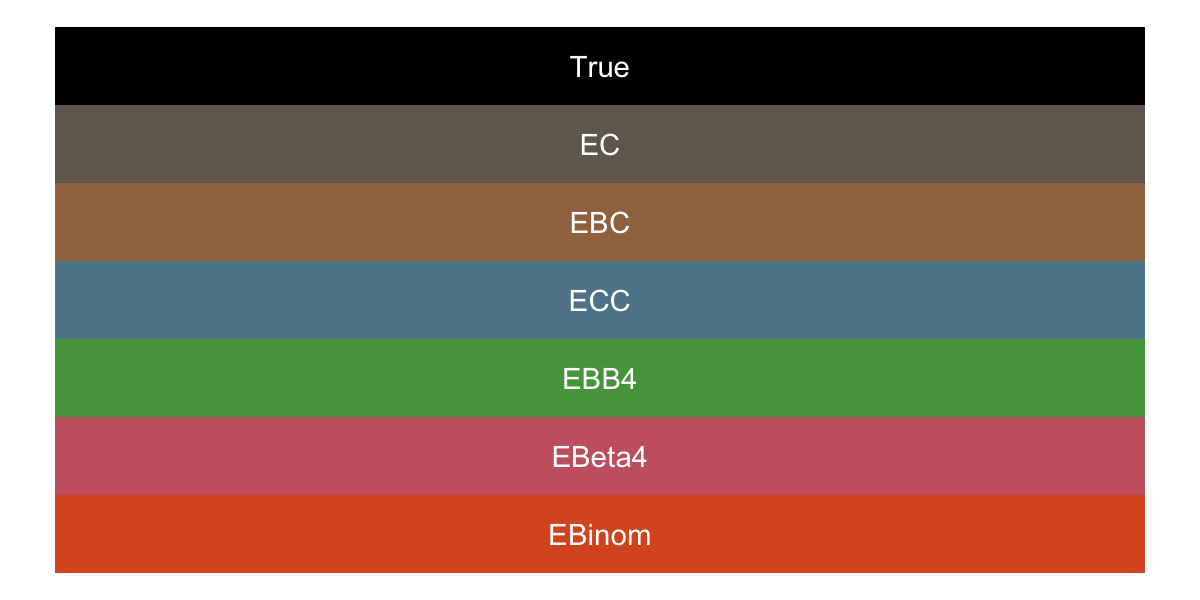
\includegraphics[width=17cm]{ColorPalette/ColorPalette.png}
\caption{Colour code mapping}
\end{figure}%

Notice that some combinations of copula, Kendall's tau and dimensions are not plotted. For instance:\\
\vspace{0.5cm}
Recall that the domain of the parameter of Clayton and Gumbel-Hougaard copula is $(0,\infty)$ and $[1,\infty)$ respectively. Consider the Kendall's tau for Gumbel-Hougaard and Clayton copulas:
\begin{align*}
    \tau_{C} = \frac{\theta}{\theta + 2}, \: \theta \in (0,\infty) \: \Longrightarrow \: \tau_{C} \in (0,\infty) \\
    \tau_{G} = \frac{\theta - 1}{\theta}, \: \theta \in [1,\infty) \: \Longrightarrow \: \tau_{G} \in [0,\infty) 
\end{align*}
Hence, we will only consider $\tau_{C} \in {0.25, 0.5, 0.75}$ for Clayton and Gumbel copulas.\\
\vspace{0.5cm}
Moreover, the rotated copula for normal and student-$t$ copulas faces Monte Carlo errors for $d \ge 3$ \parencite{HofertBook}, hence we will only consider normal and student-$t$ copulas at $d = 2$.
\newpage
\subsection{Plots: exceedance probabilities vs $\textbf{u}$ (evaluation points)}
\vspace{0.5cm}
We first plot the (upper-tailed) evaluation points against the exceedance probabilities for each empirical copula. The evaluation points are on the x-axis and the exceedance probabilities are on the y-axis. The solid line is the mean of the exceedance probabilities corresponding to the evaluation point, and the dotted line is the confidence intervals of the exceedance probabilities corresponding to the evaluation point.

\begin{center}
\label{t4_2d_s}
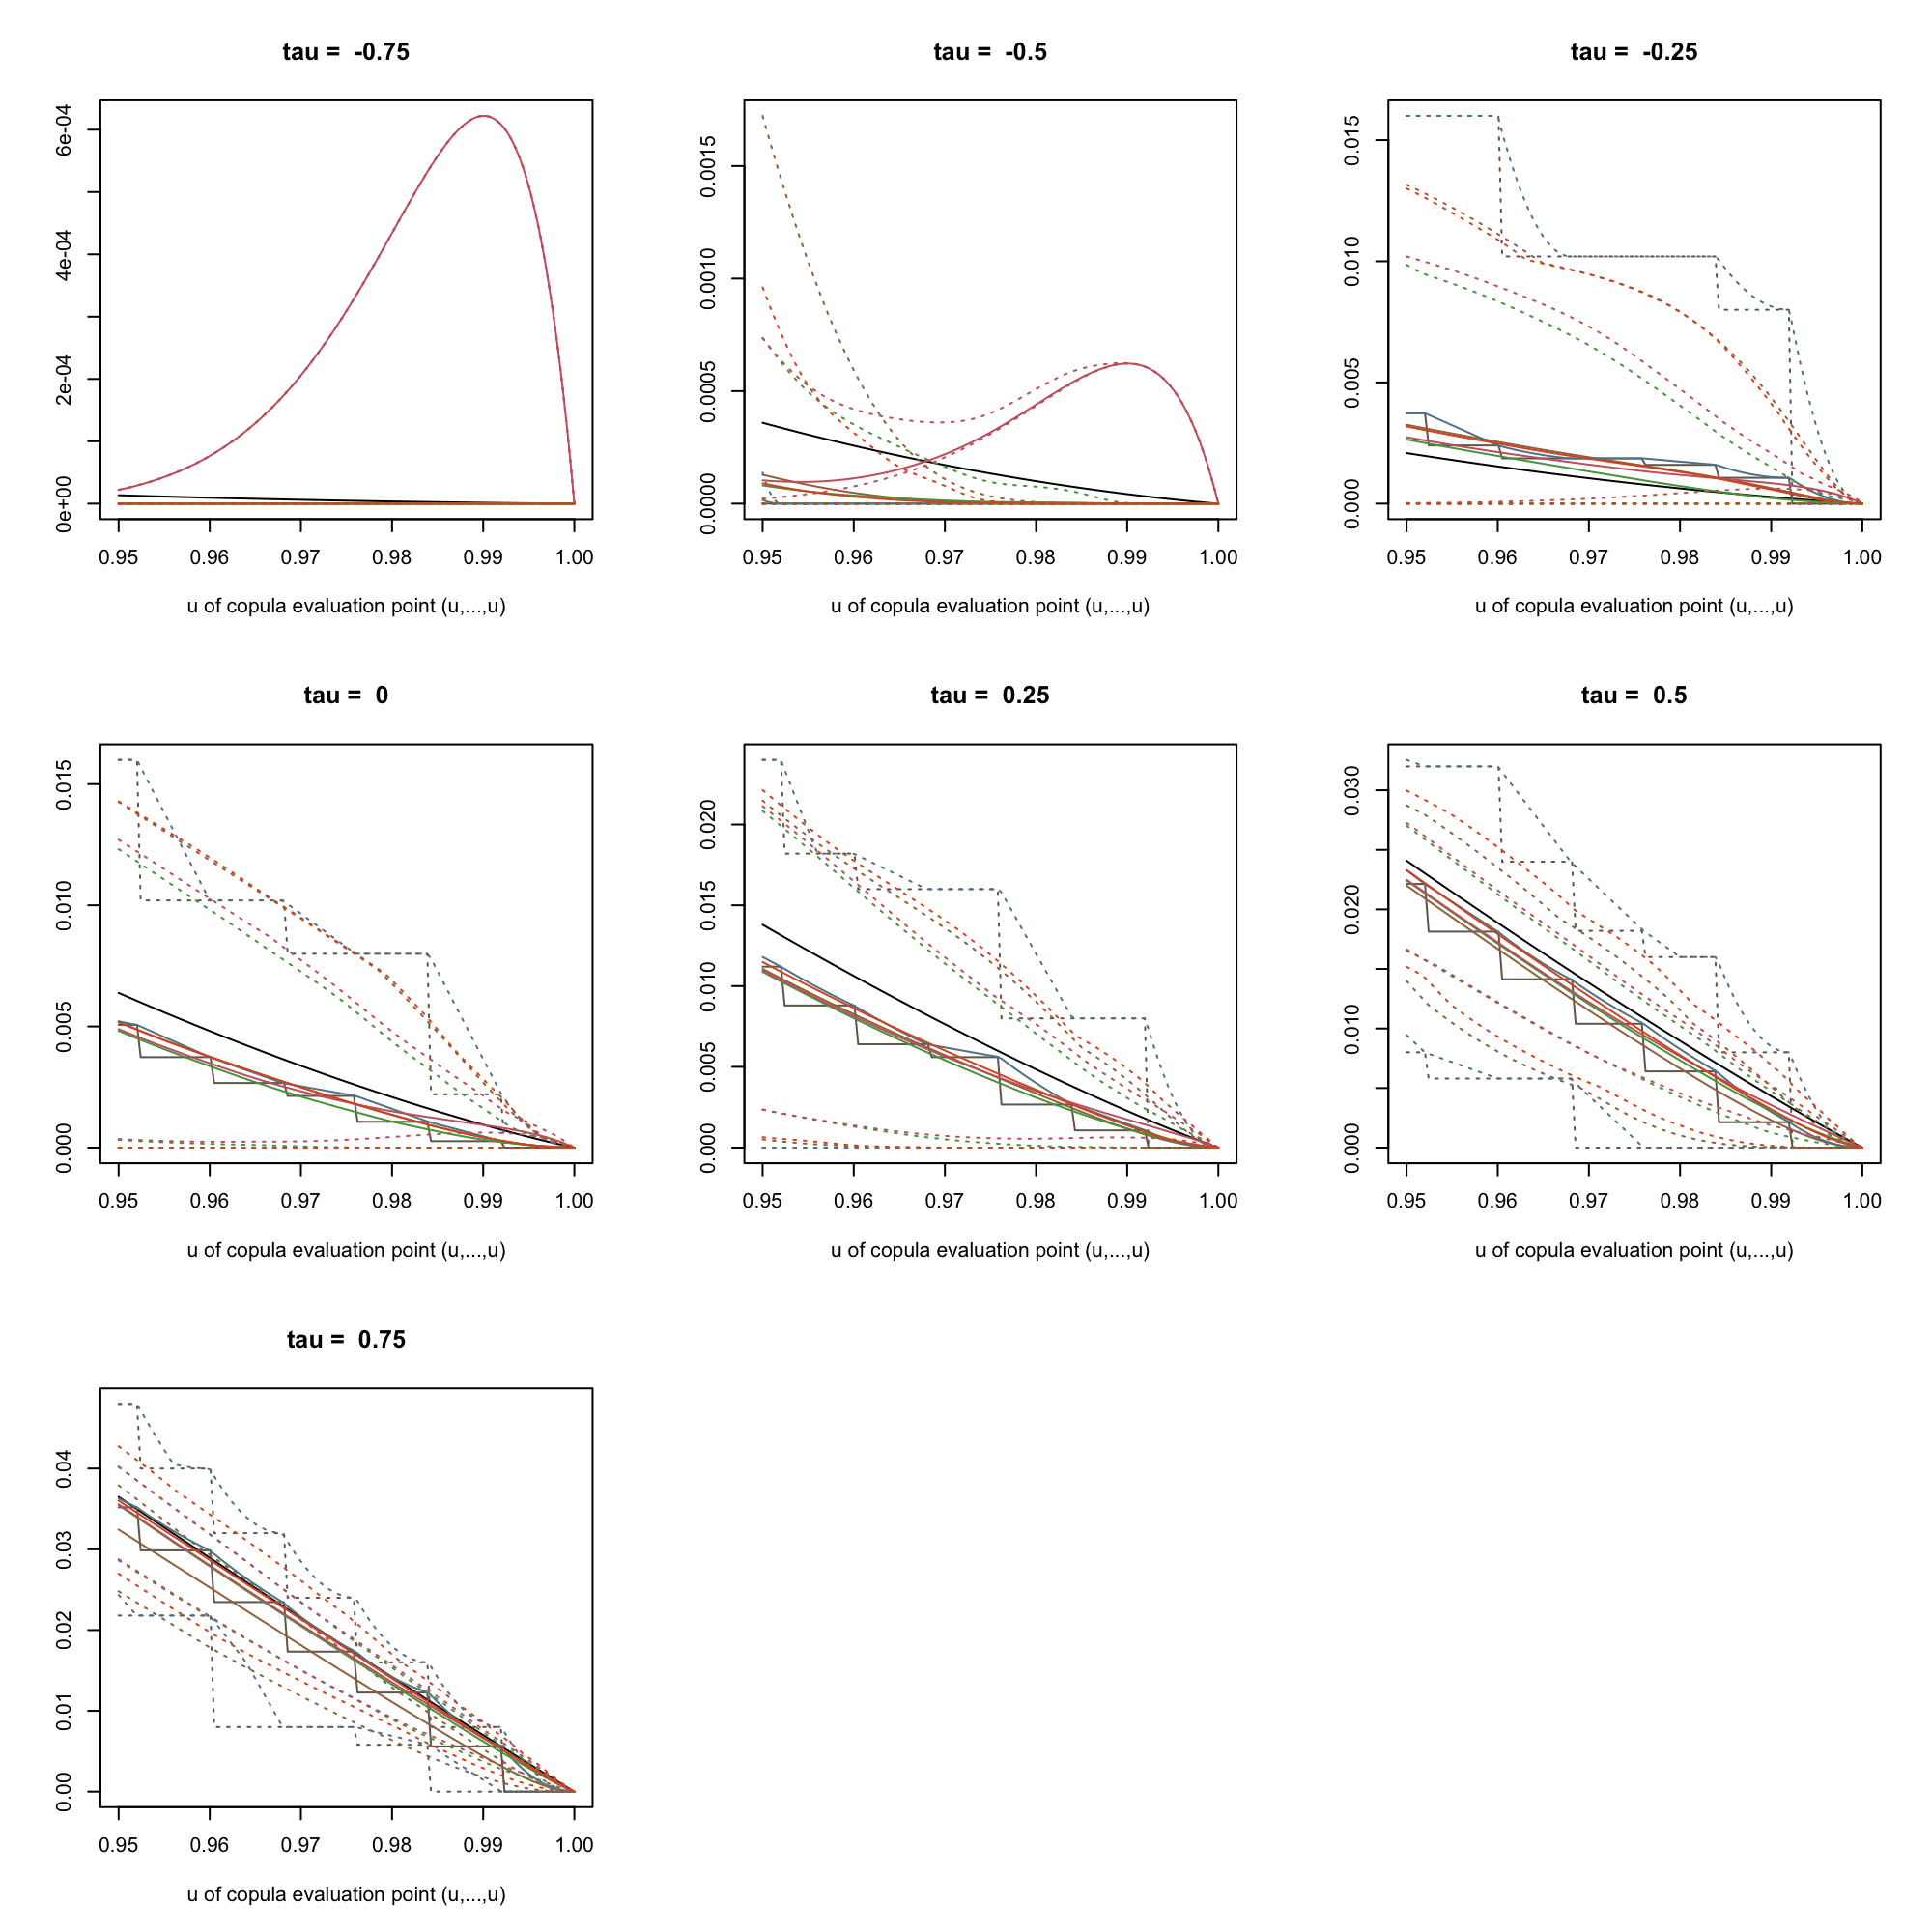
\includegraphics[width=17cm]{ExceedanceProb/t4_2d_s.png}
\captionof{figure}{Student-$t$ copula with $d$ = 2}
\end{center}%

\begin{center}
\label{N_2d_s}
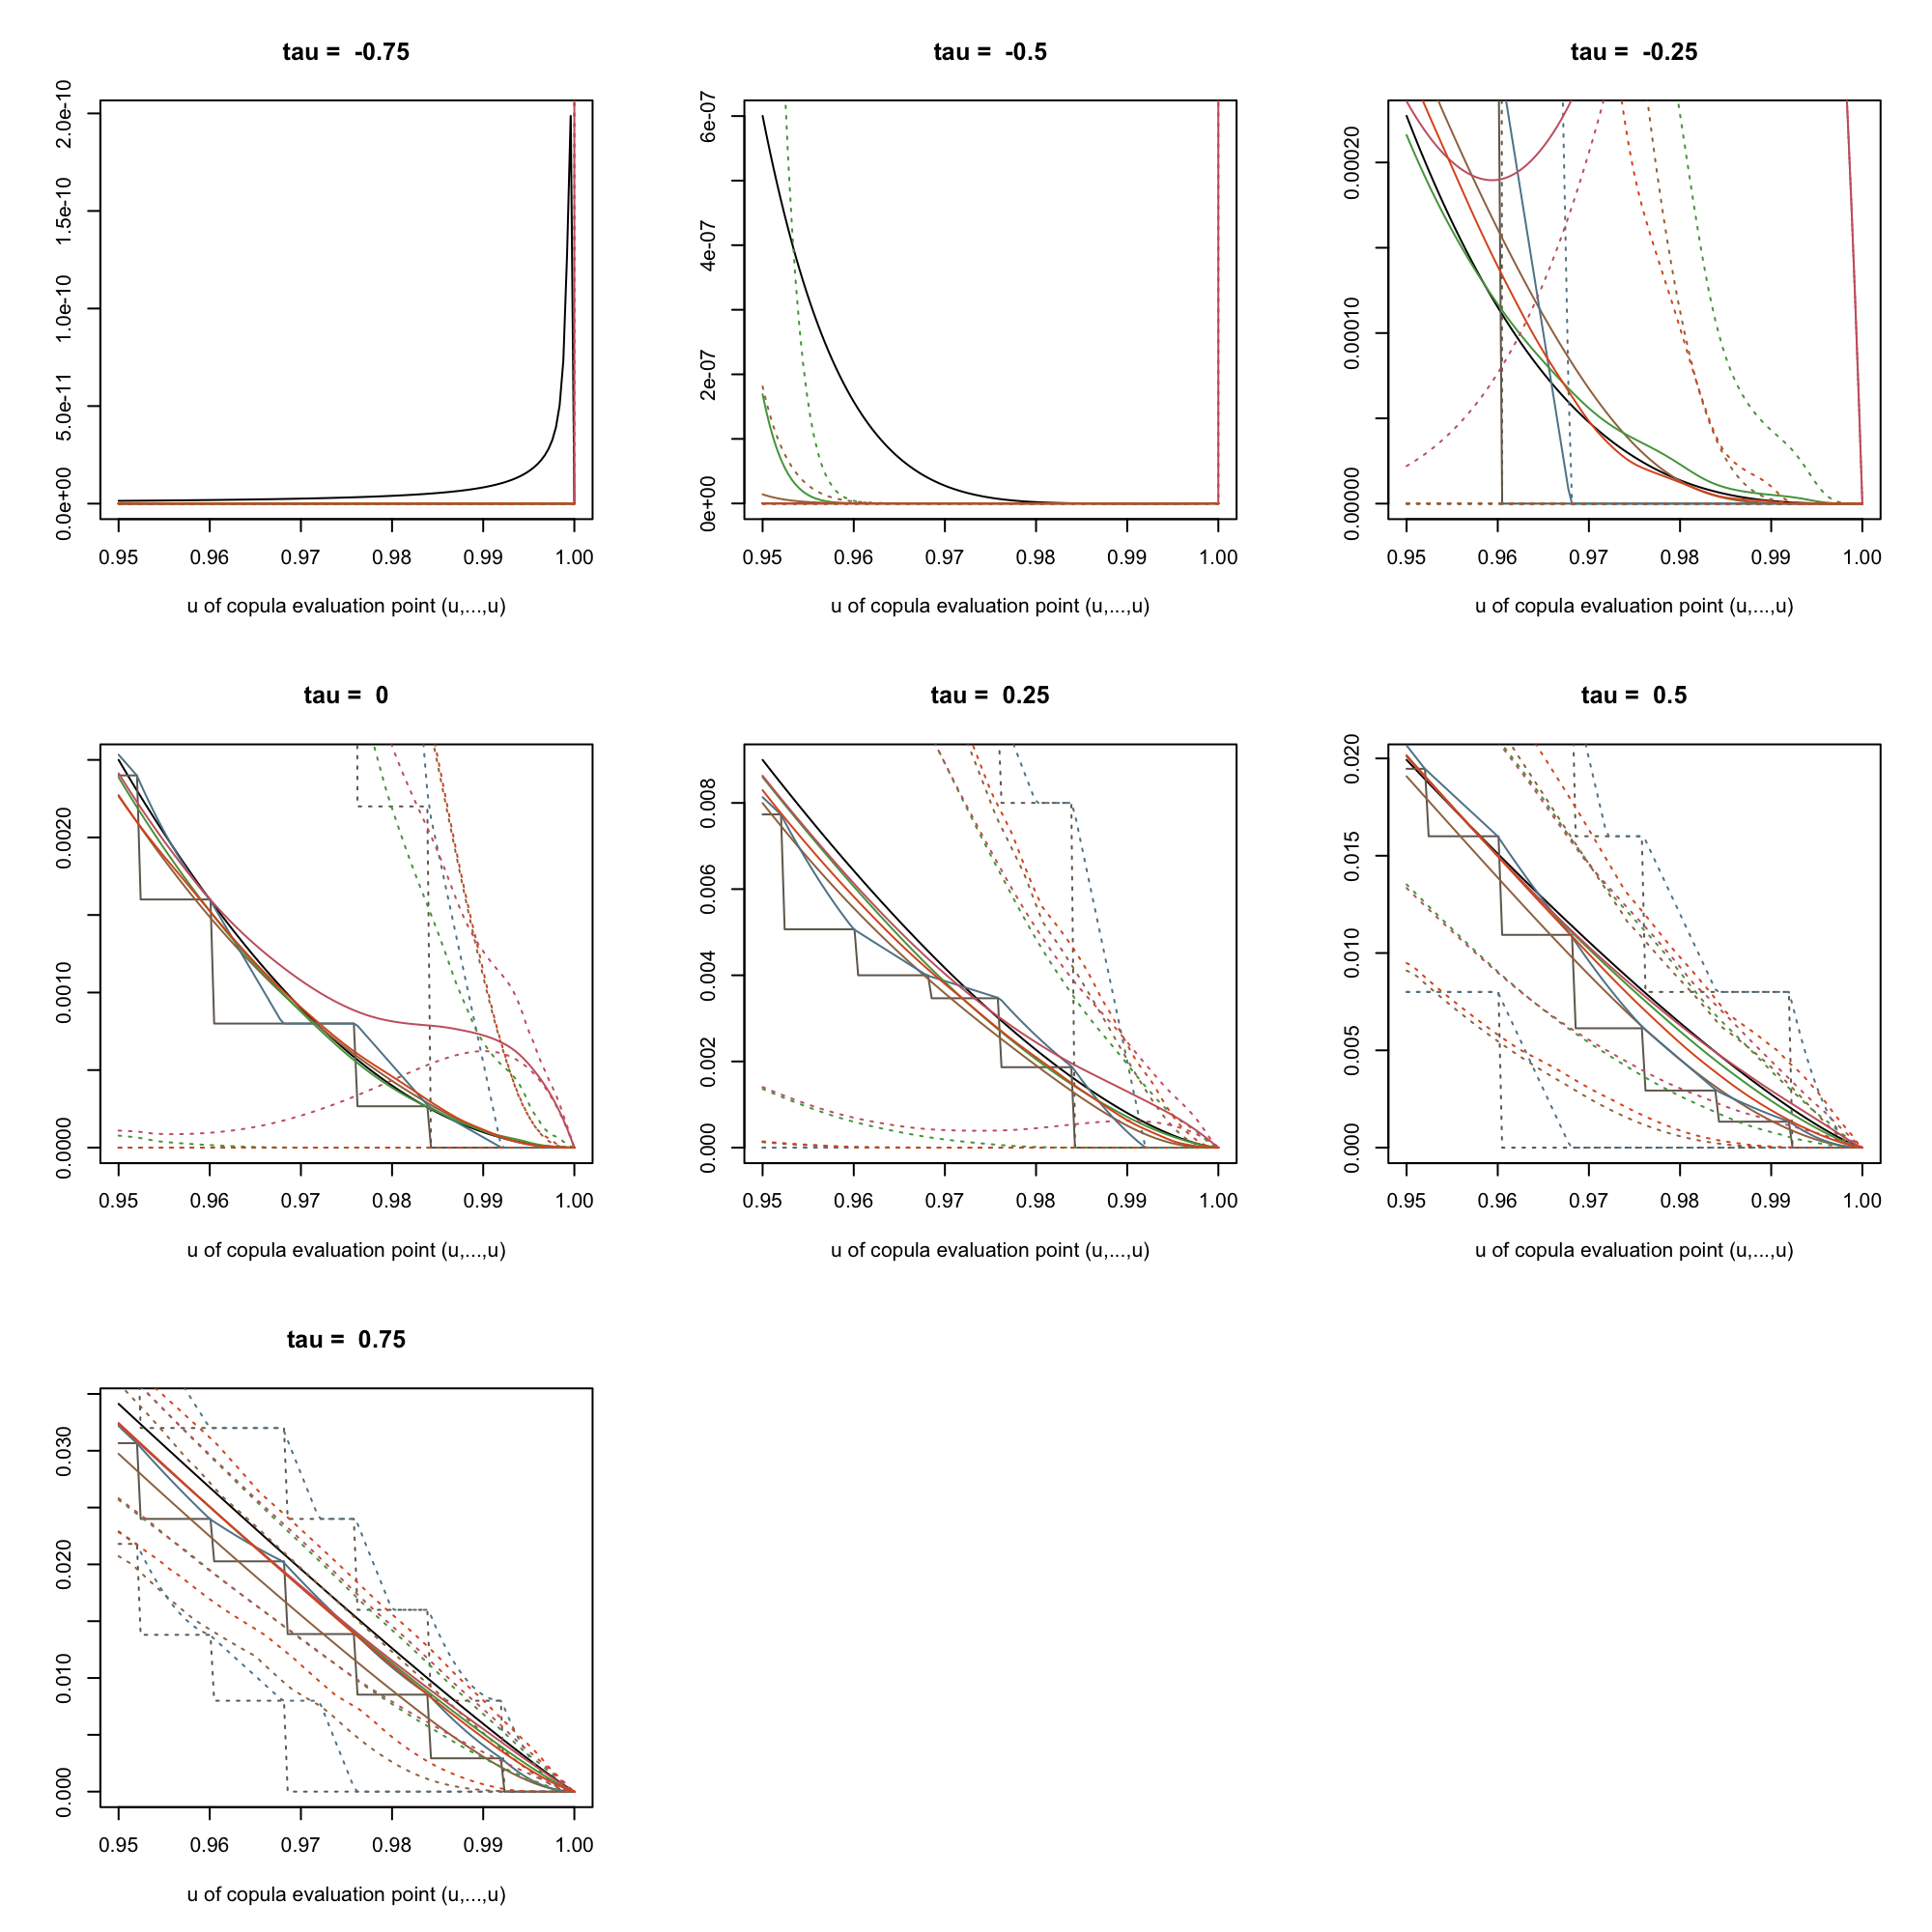
\includegraphics[width=17cm]{ExceedanceProb/N_2d_s.png}
\captionof{figure}{Gaussian copula with $d$ = 2}
\end{center}%

\begin{center}
\label{G_2d_s}
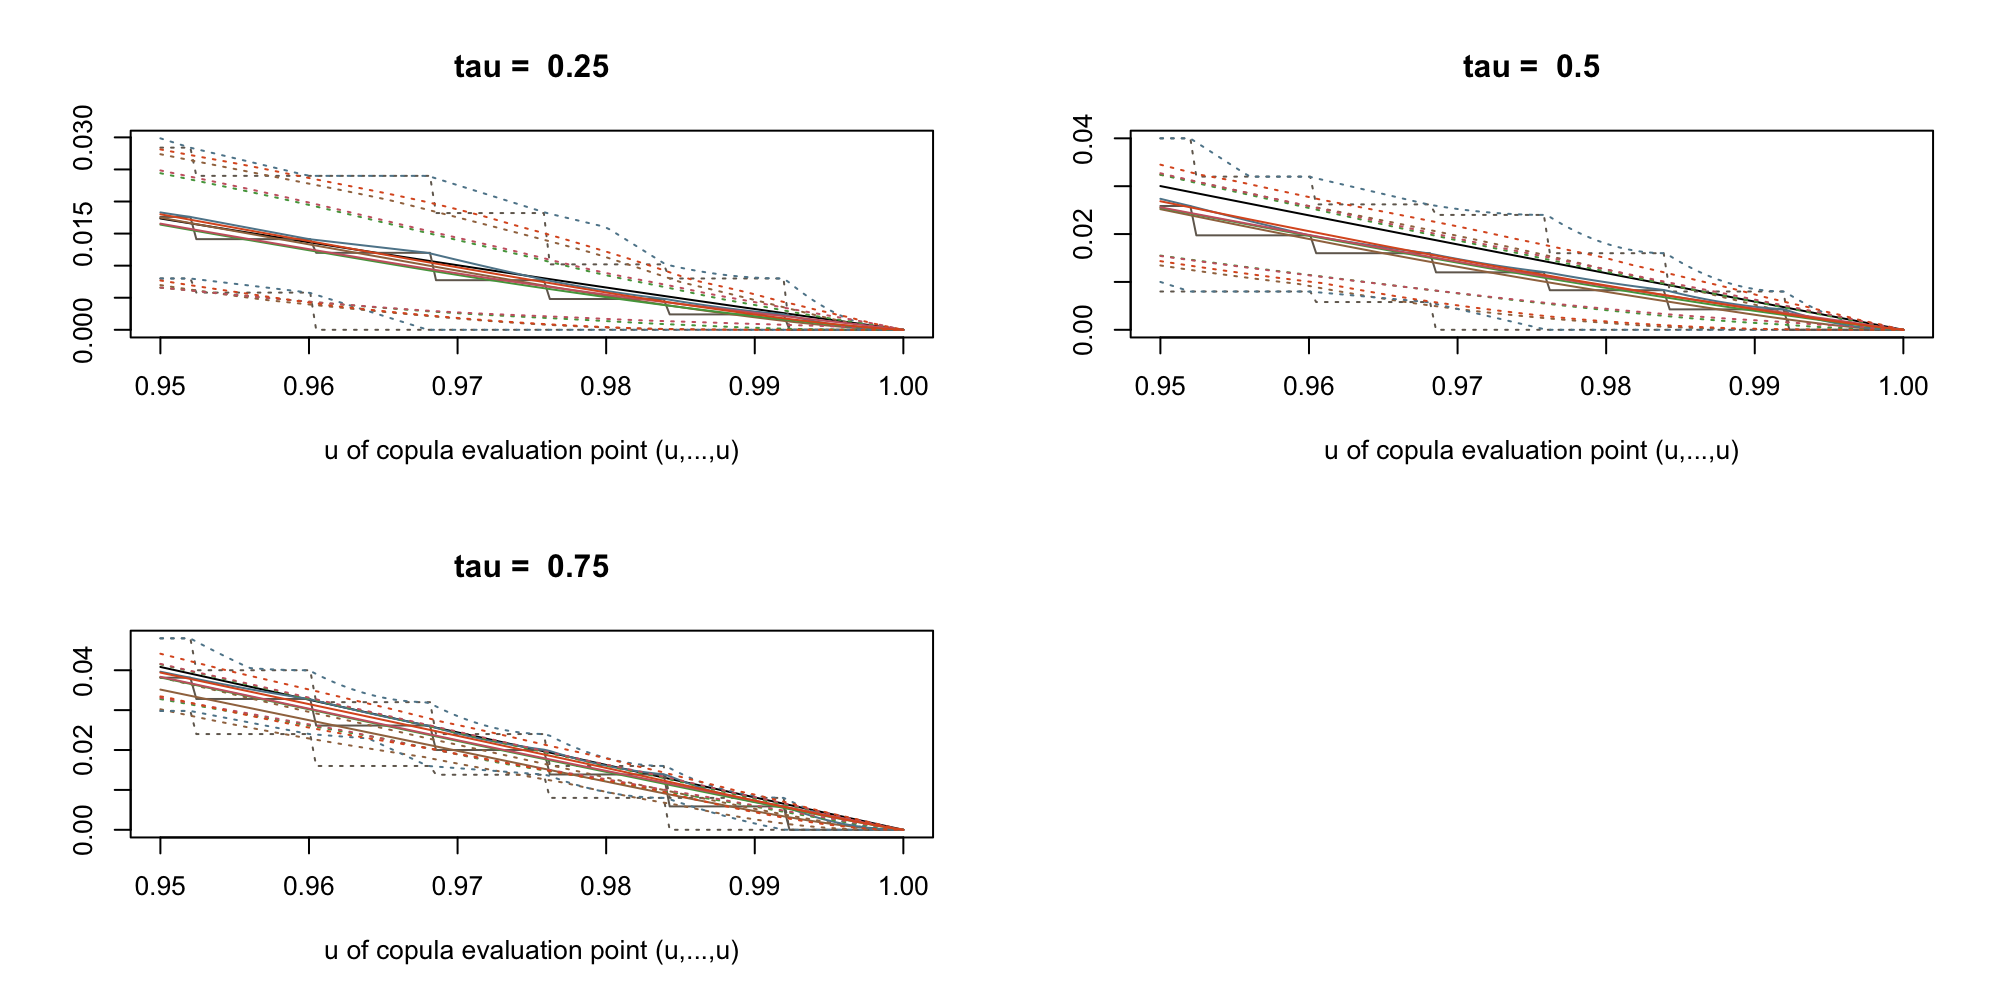
\includegraphics[width=17cm]{ExceedanceProb/G_2d_s.png}
\captionof{figure}{Gumbel-Hougaard copula with $d$ = 2}
\end{center}%

\begin{center}
\label{G_3d_s}
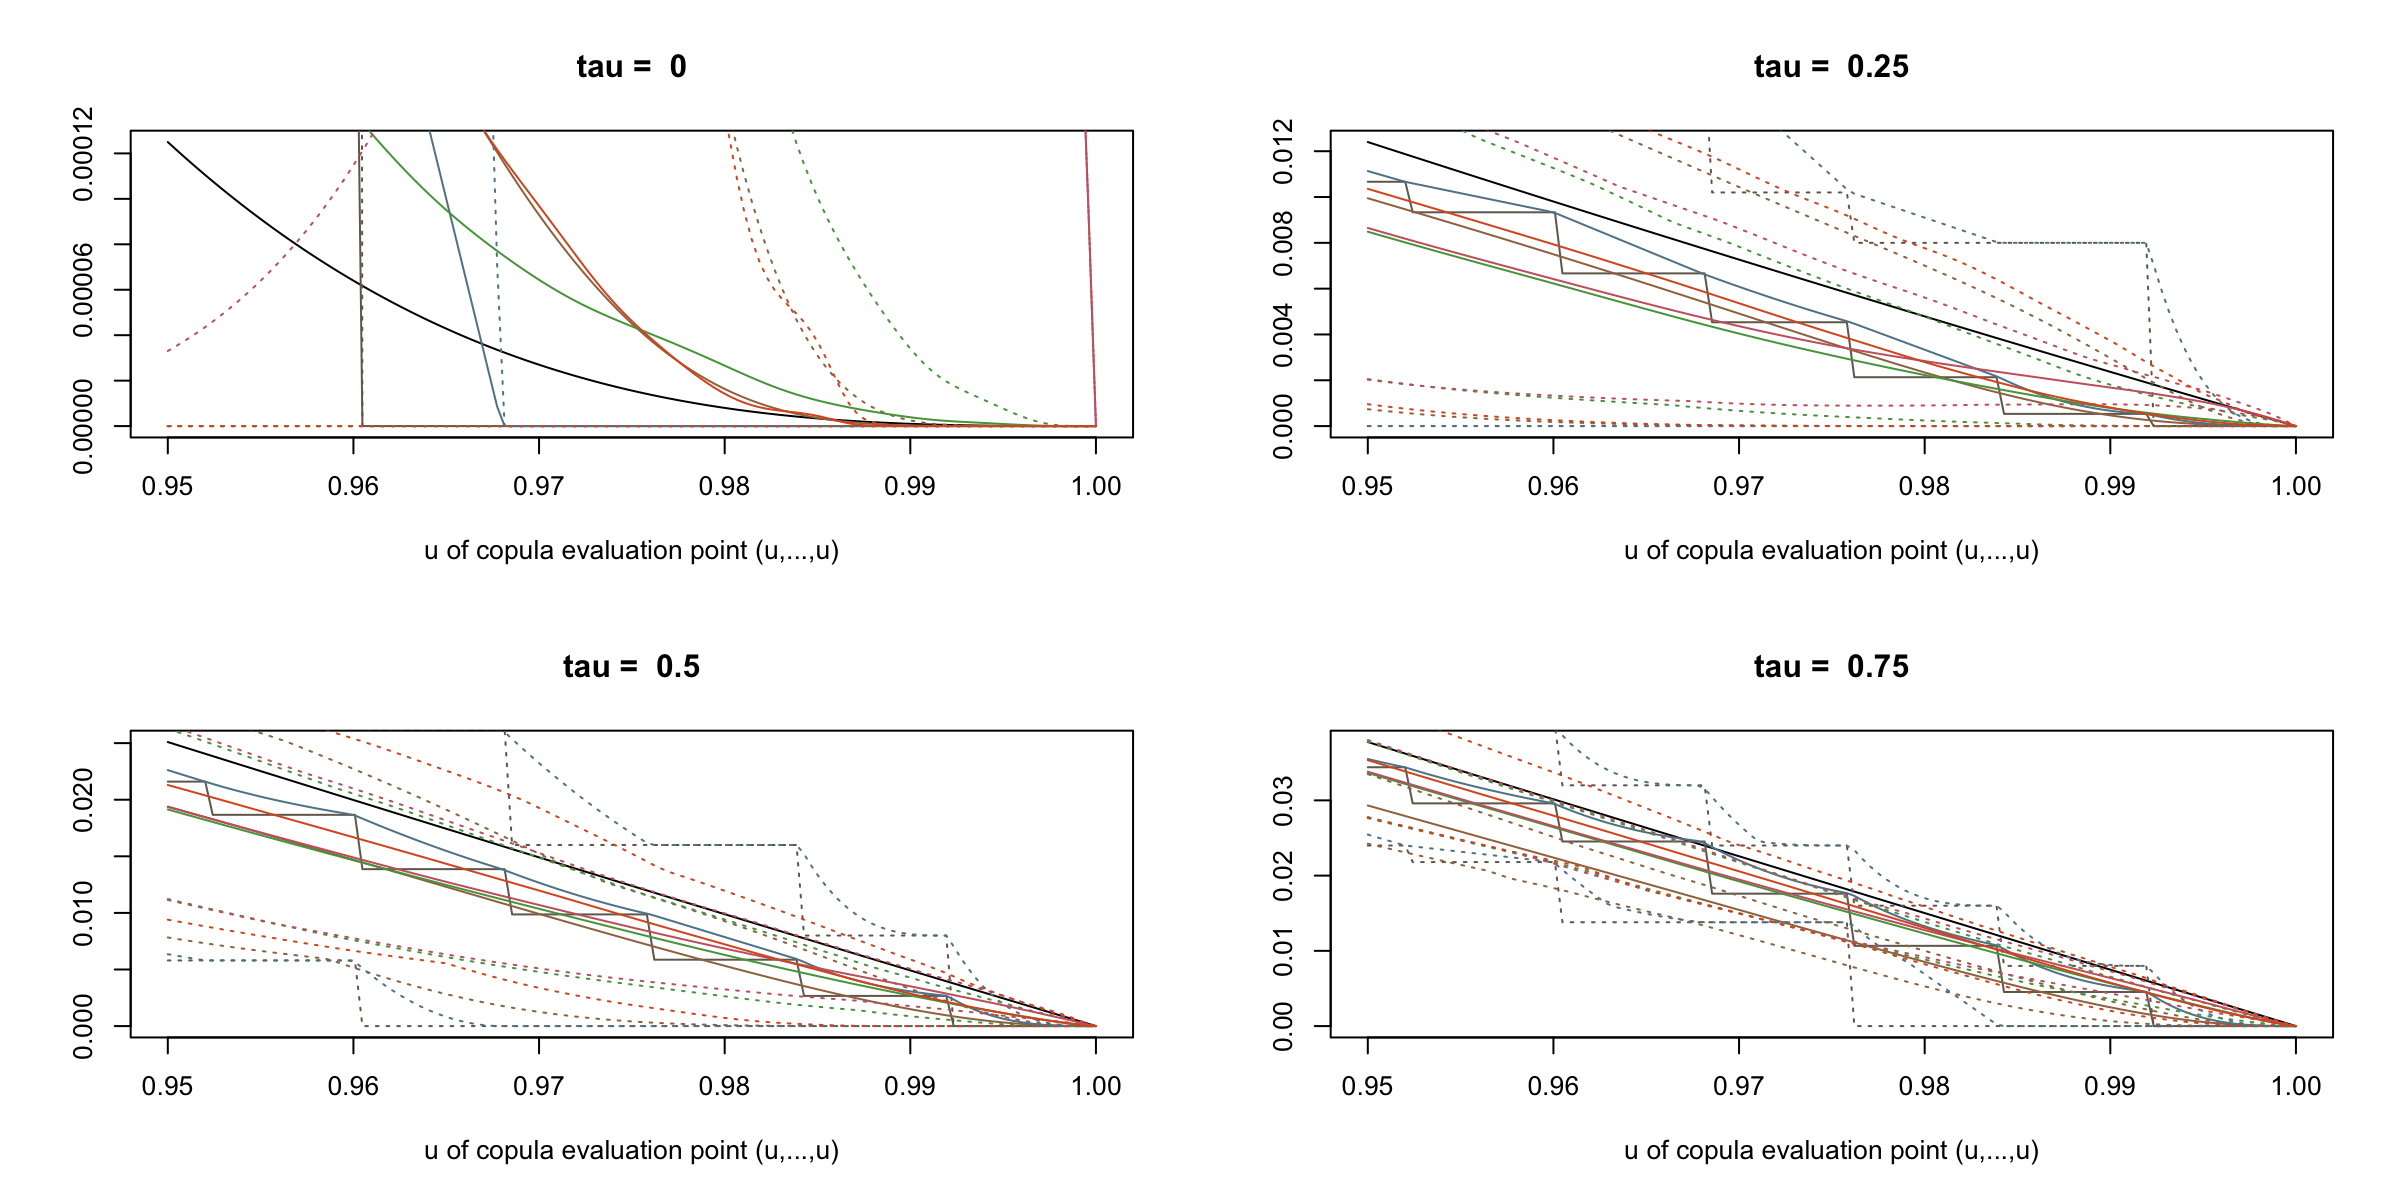
\includegraphics[width=17cm]{ExceedanceProb/G_3d_s.png}
\captionof{figure}{Gumbel-Hougaard copula with $d$ = 3}
\end{center}%

\begin{center}
\label{G_4d_s}
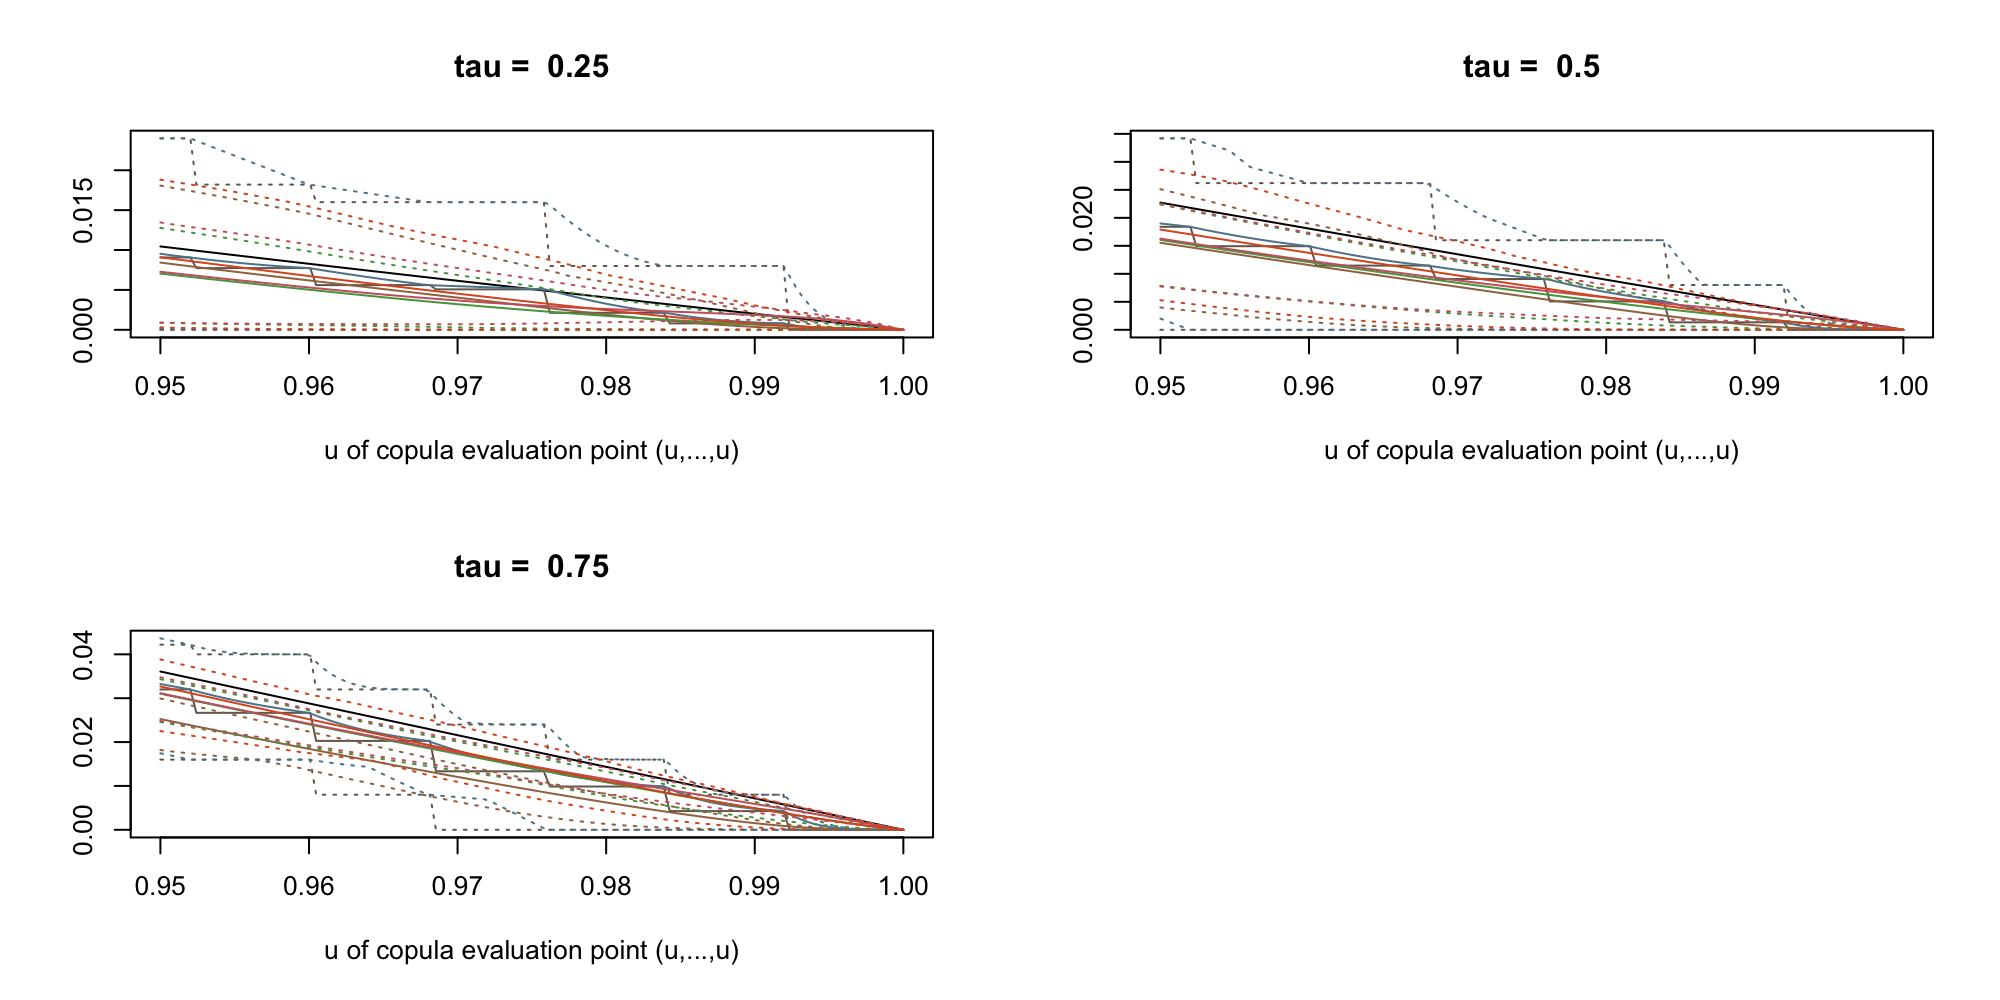
\includegraphics[width=17cm]{ExceedanceProb/G_4d_s.png}
\captionof{figure}{Gumbel-Hougaard copula with $d$ = 4}
\end{center}%

\begin{center}
\label{G_5d_s}
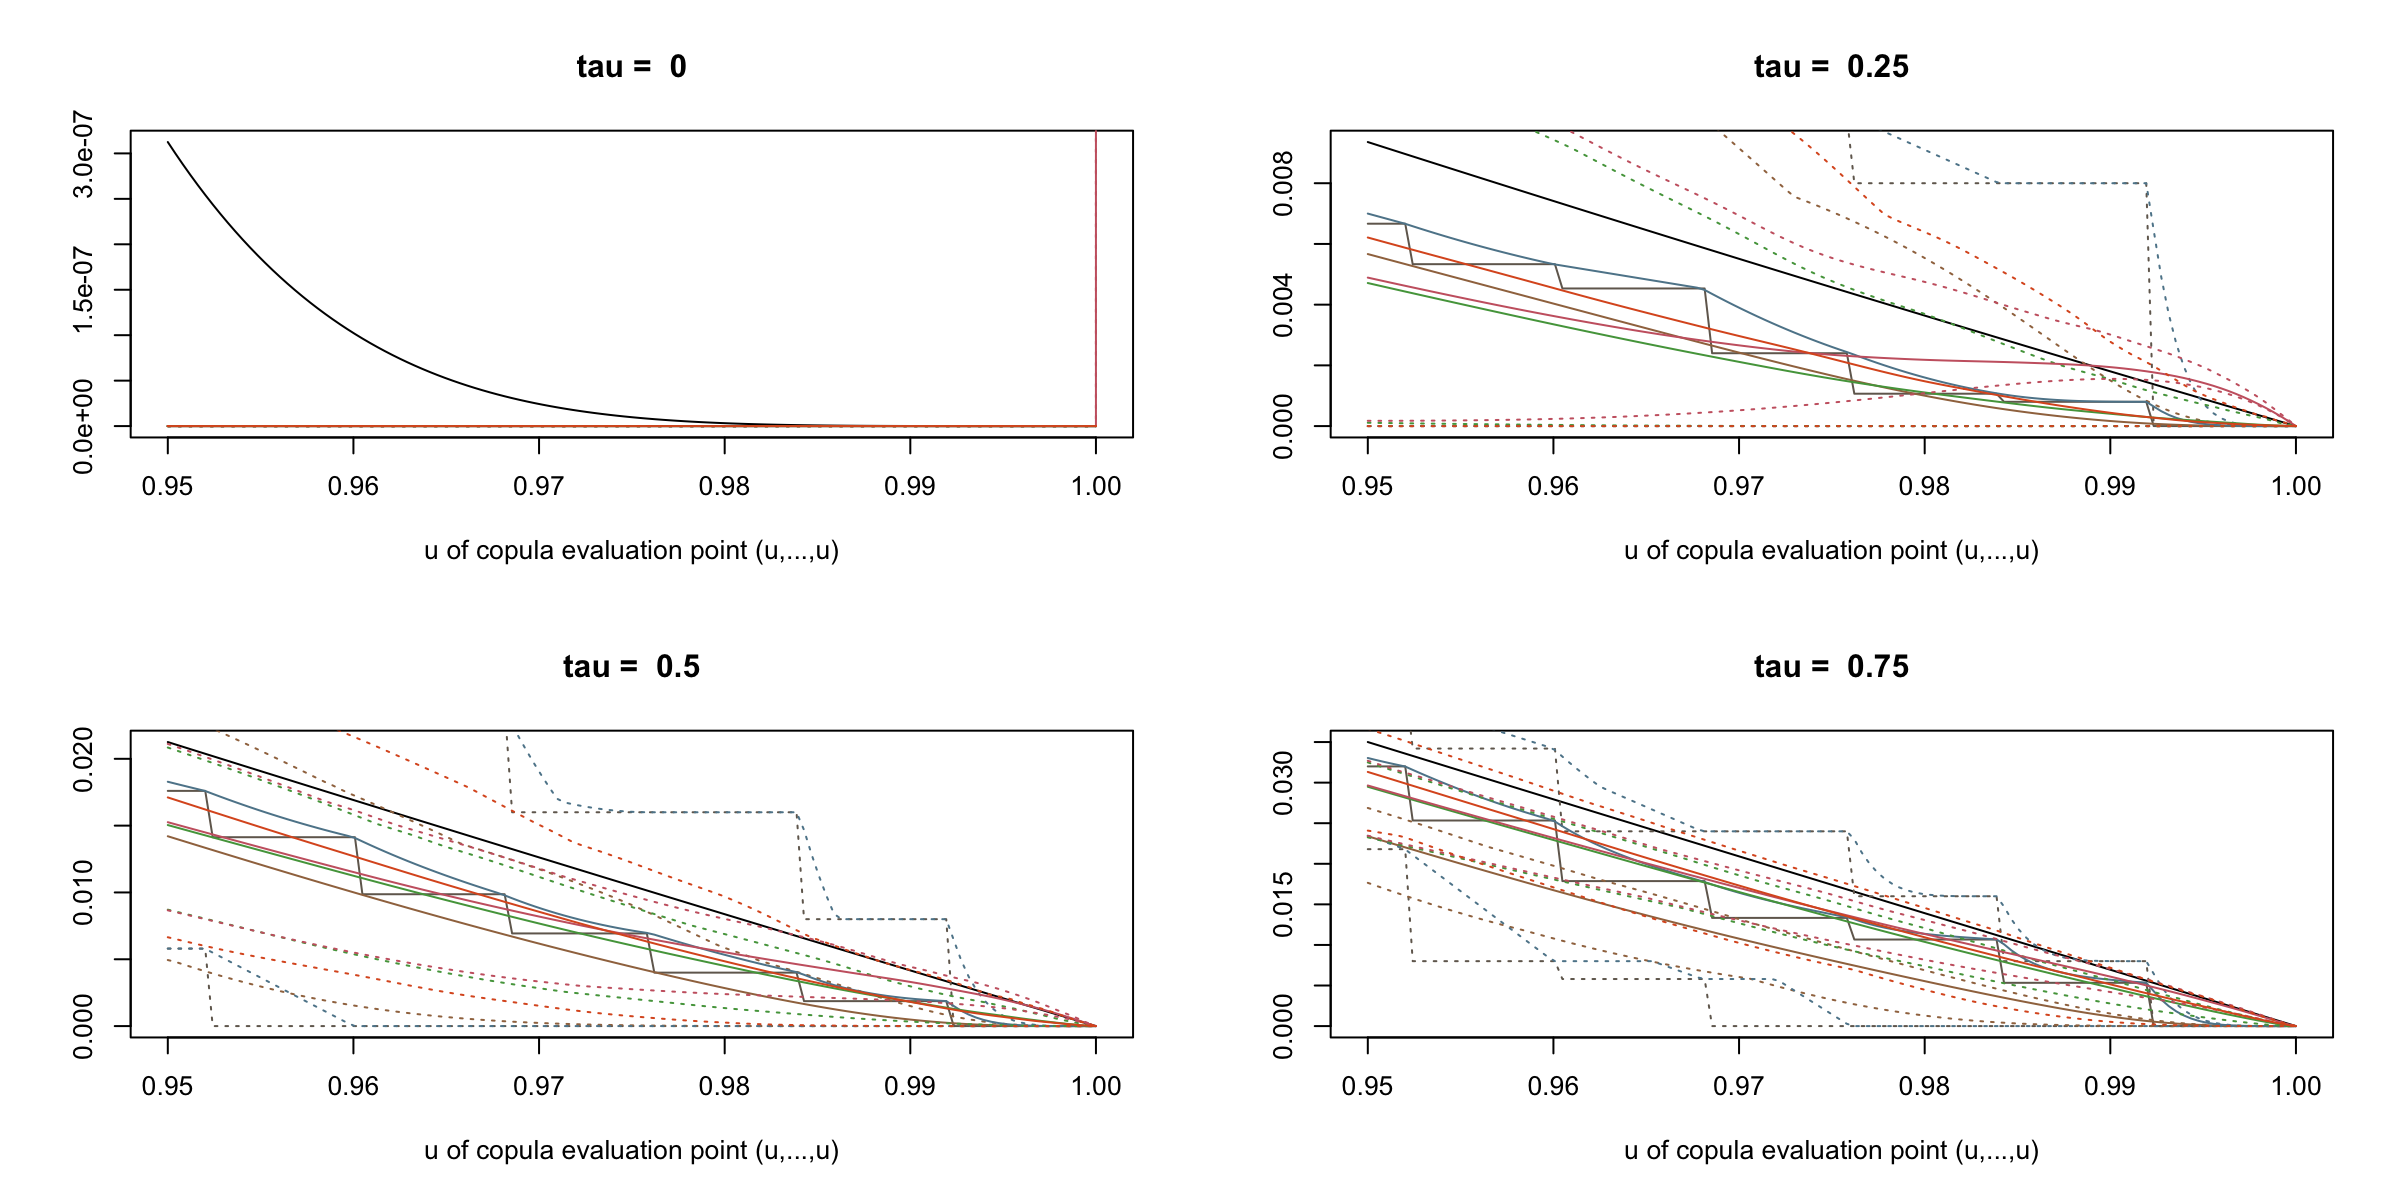
\includegraphics[width=17cm]{ExceedanceProb/G_5d_s.png}
\captionof{figure}{Gumbel-Hougaard copula with $d$ = 5}
\end{center}%

\newpage
\subsection{CvM: Exceedance probabilities}
To better understand the proximity of the exceedance probabilities from the class of empirical copula, with respect to the true copula, we then compute the Cramer-von-Mises statistics for all combinations of empirical copulas, Kendall's Tau and dimensions.

\begin{center}
\label{t4_2d_s_CvM}
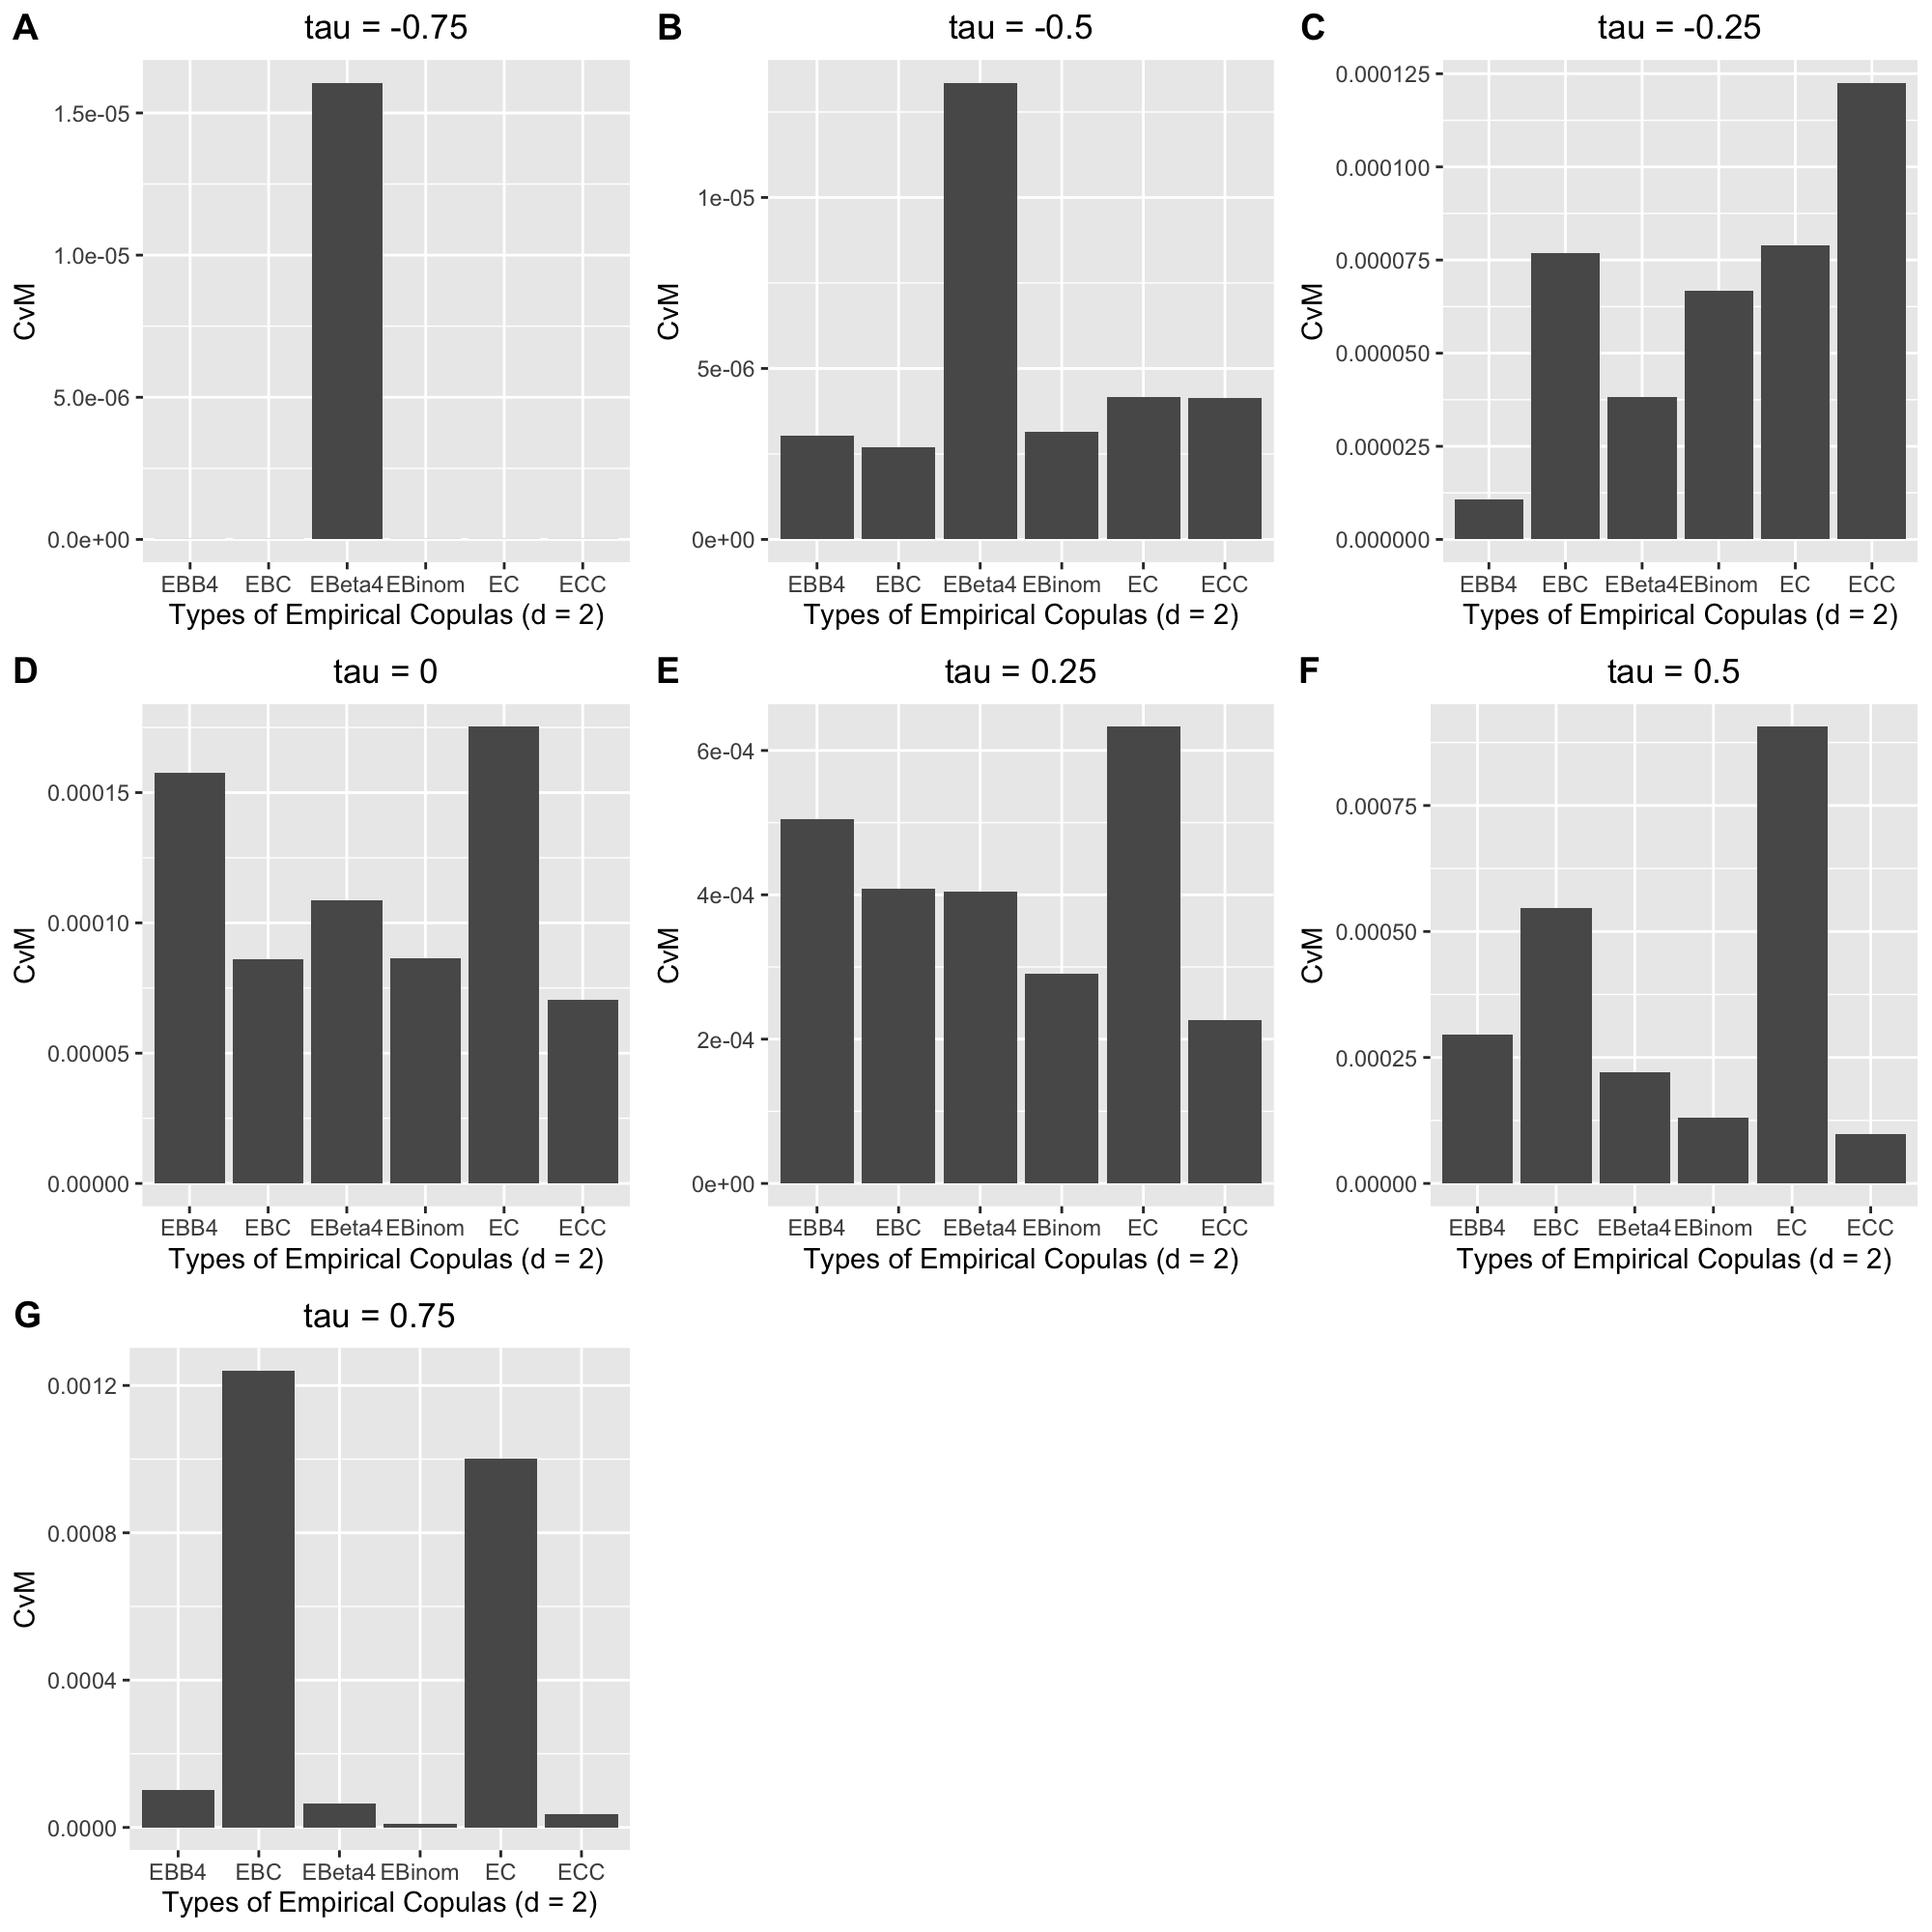
\includegraphics[width=17cm]{ExceedanceCvM/t4_2d_s_CvM.png}
\captionof{figure}{Student-$t$ copula with $d$ = 2}
\end{center}%

\begin{center}
\label{N_2d_s_CvM}
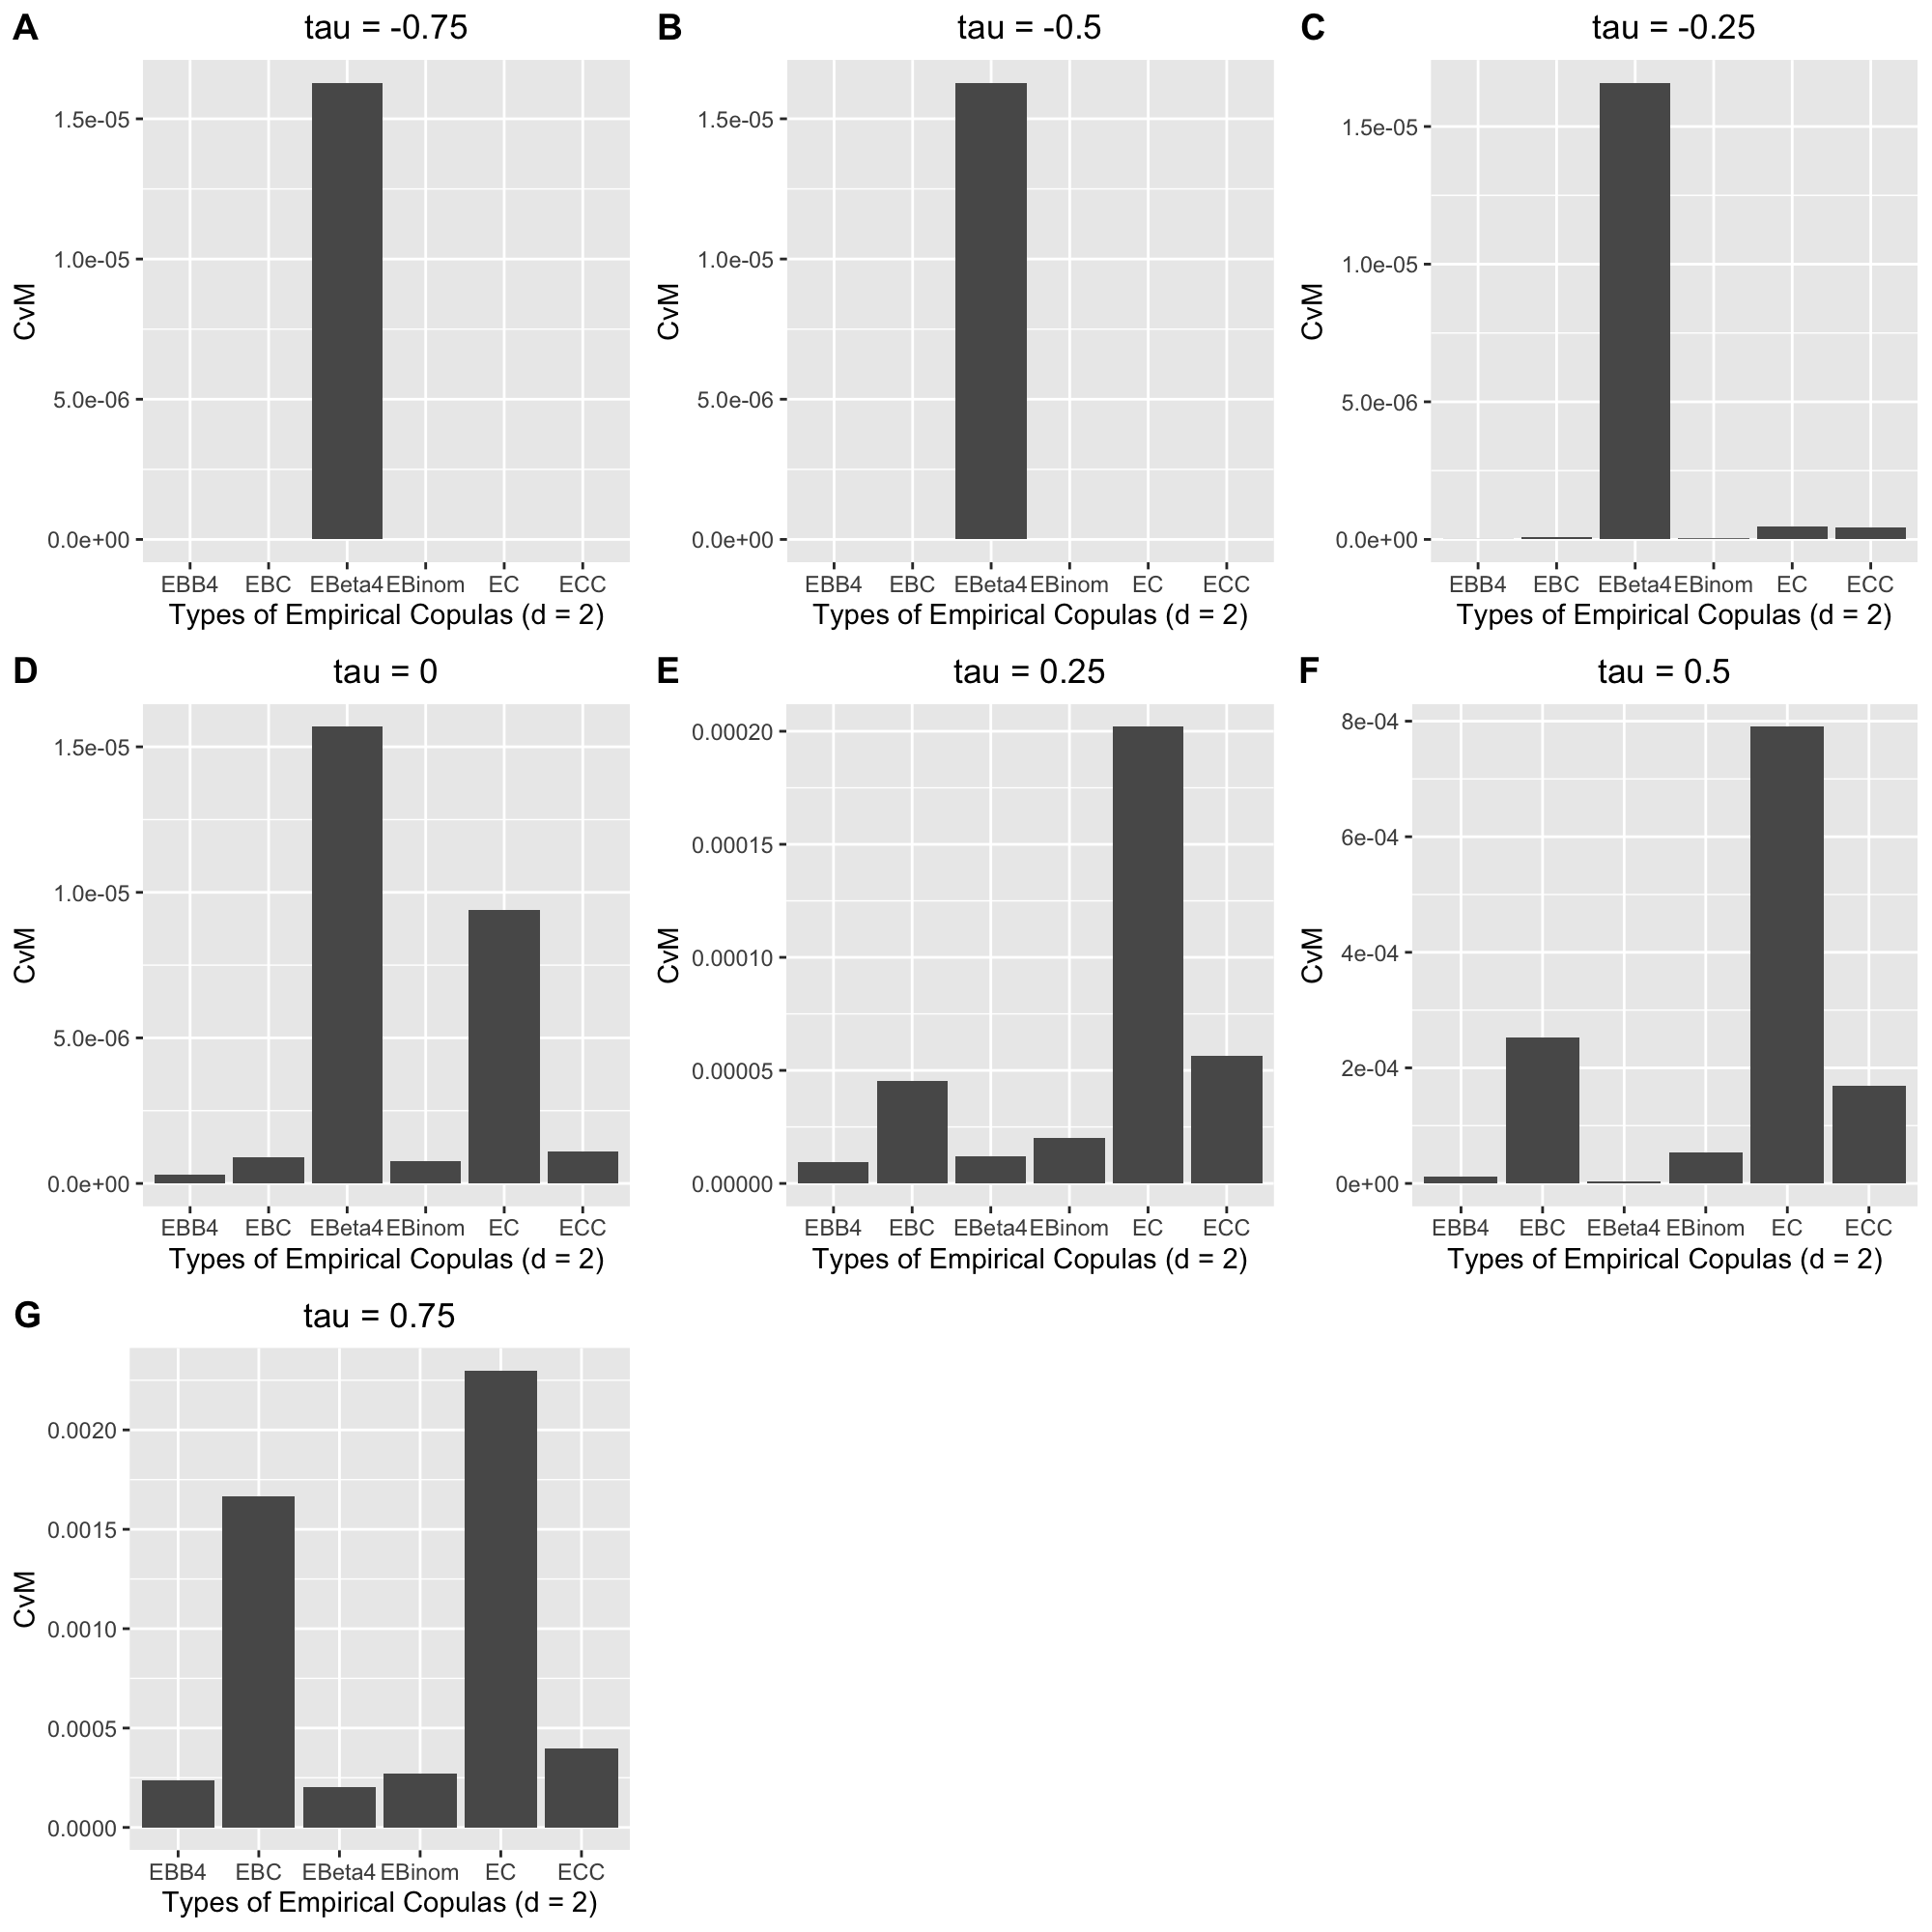
\includegraphics[width=17cm]{ExceedanceCvM/N_2d_s_CvM.png}
\captionof{figure}{Gaussian copula with $d$ = 2}
\end{center}%

\begin{center}
\label{G_2d_s_CvM}
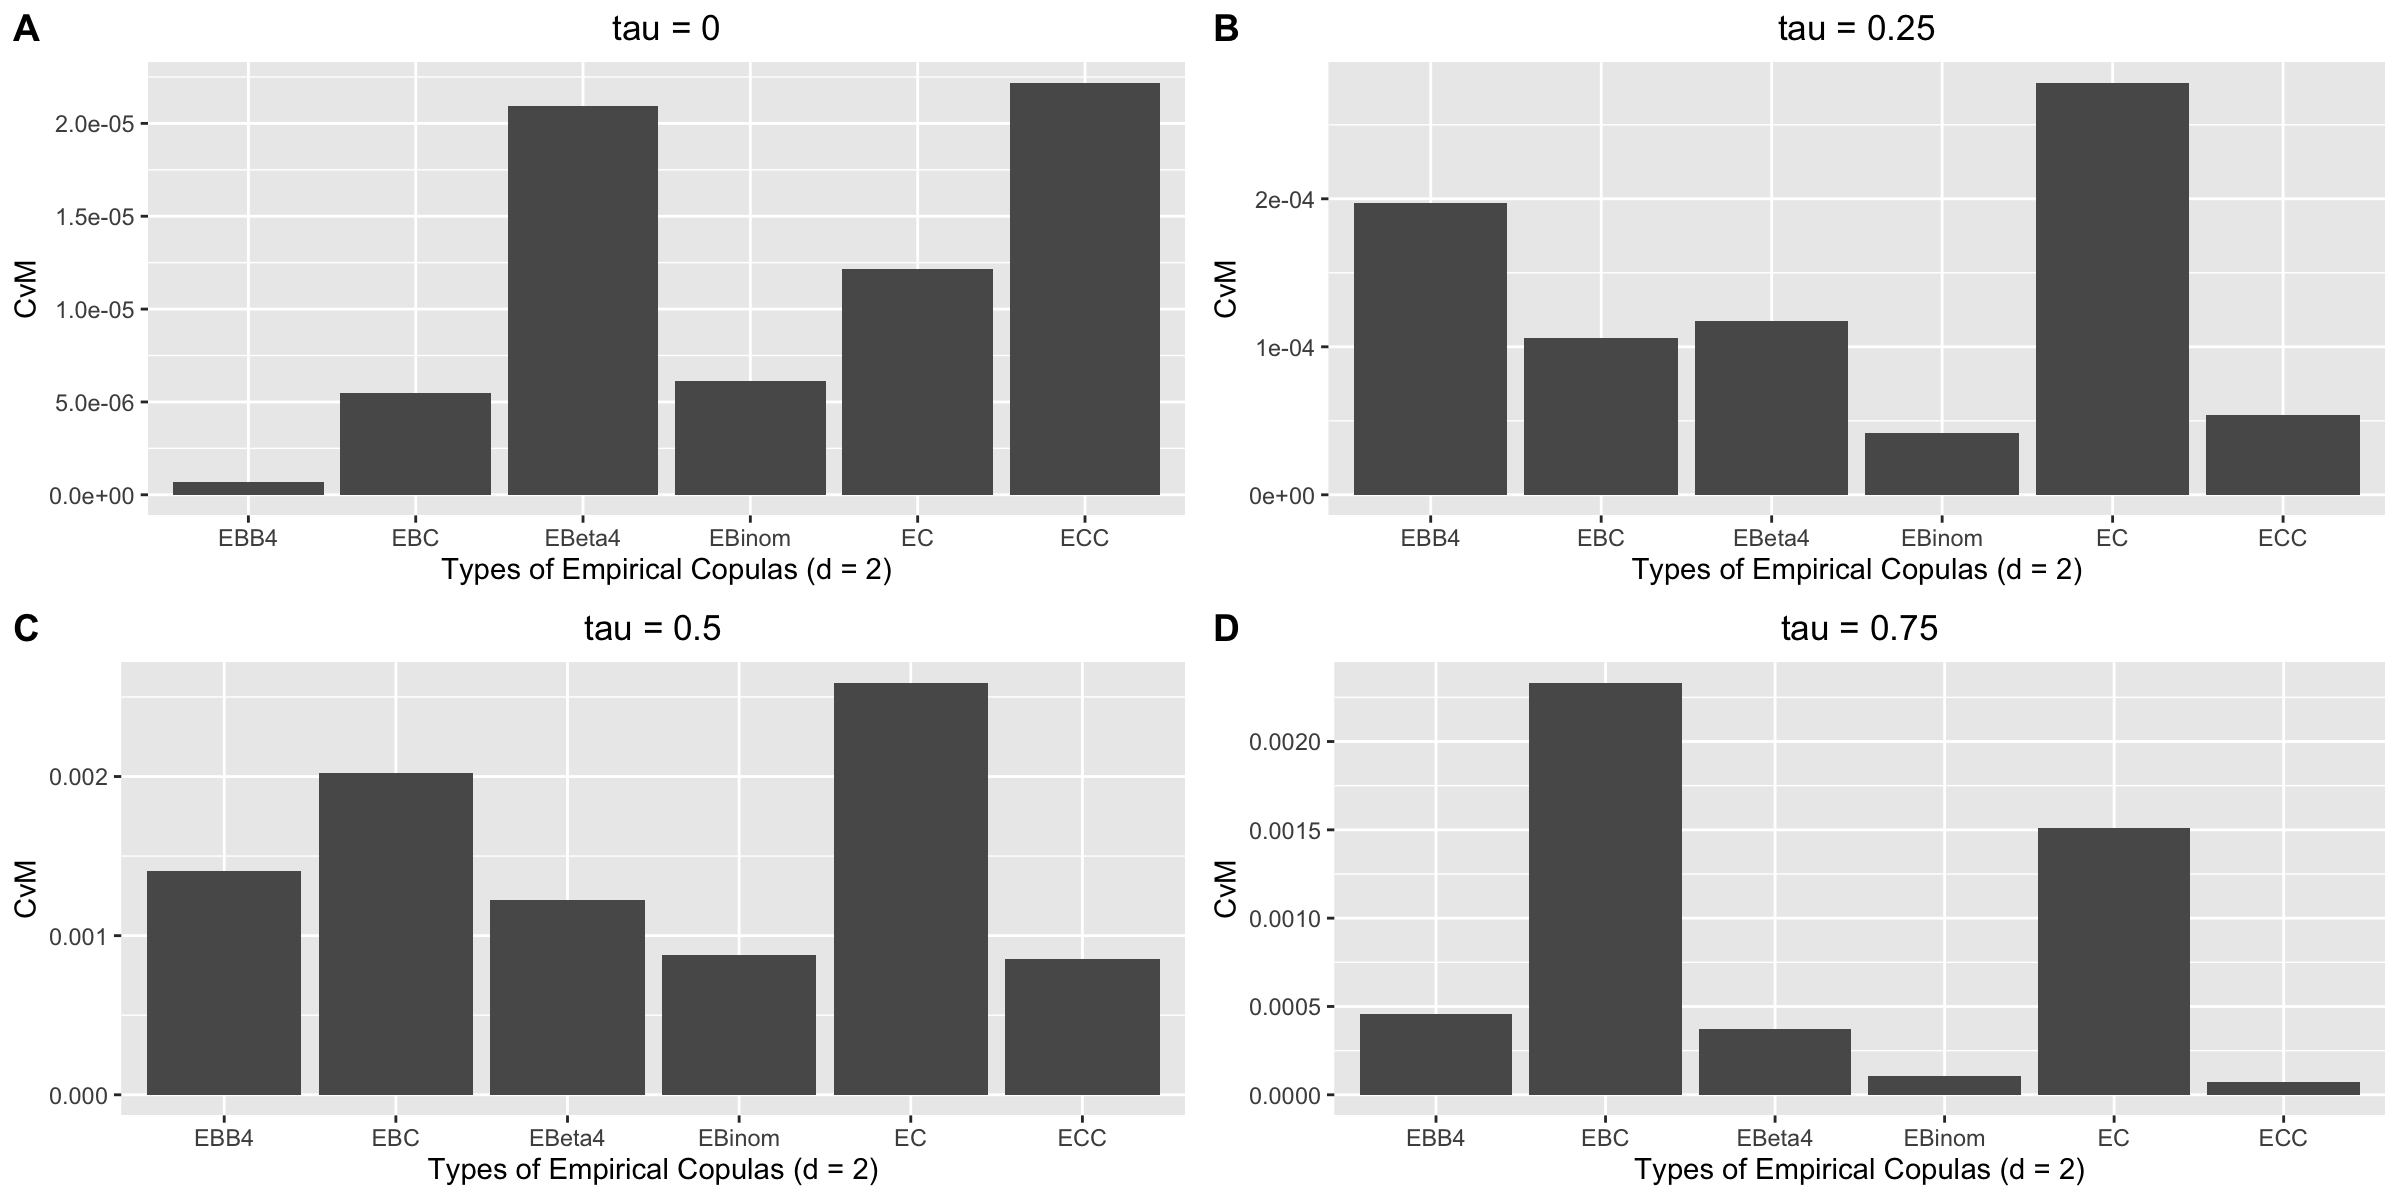
\includegraphics[width=17cm]{ExceedanceCvM/G_2d_s_CvM.png}
\captionof{figure}{Gumbel-Hougaard copula with $d$ = 2}
\end{center}%

\begin{center}
\label{G_3d_s_CvM}
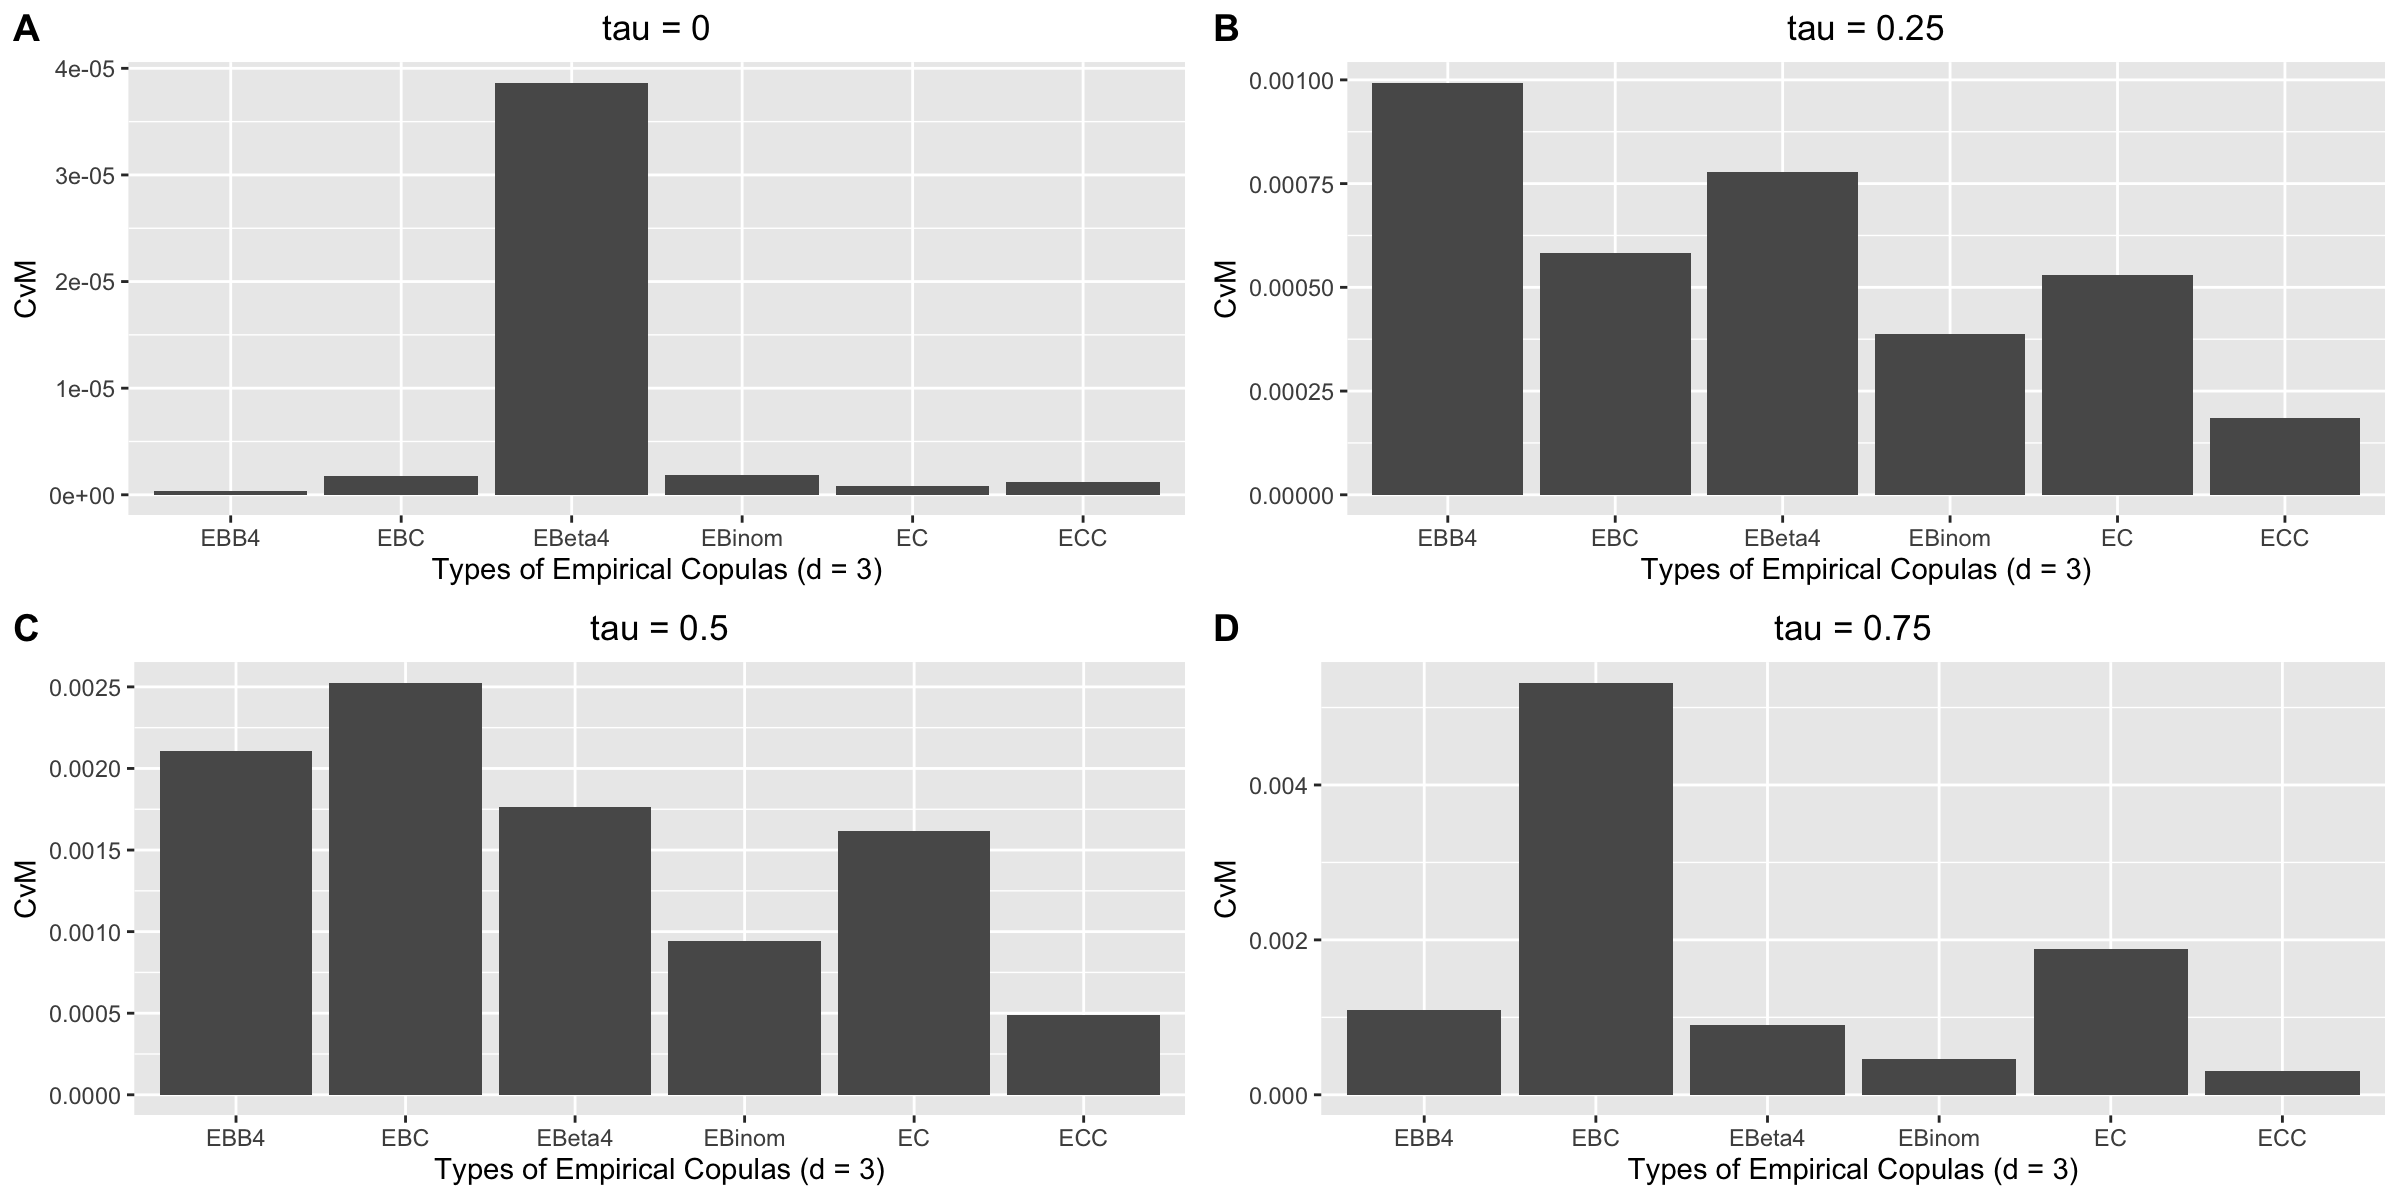
\includegraphics[width=17cm]{ExceedanceCvM/G_3d_s_CvM.png}
\captionof{figure}{Gumbel-Hougaard copula with $d$ = 3}
\end{center}%

\begin{center}
\label{G_4d_s_CvM}
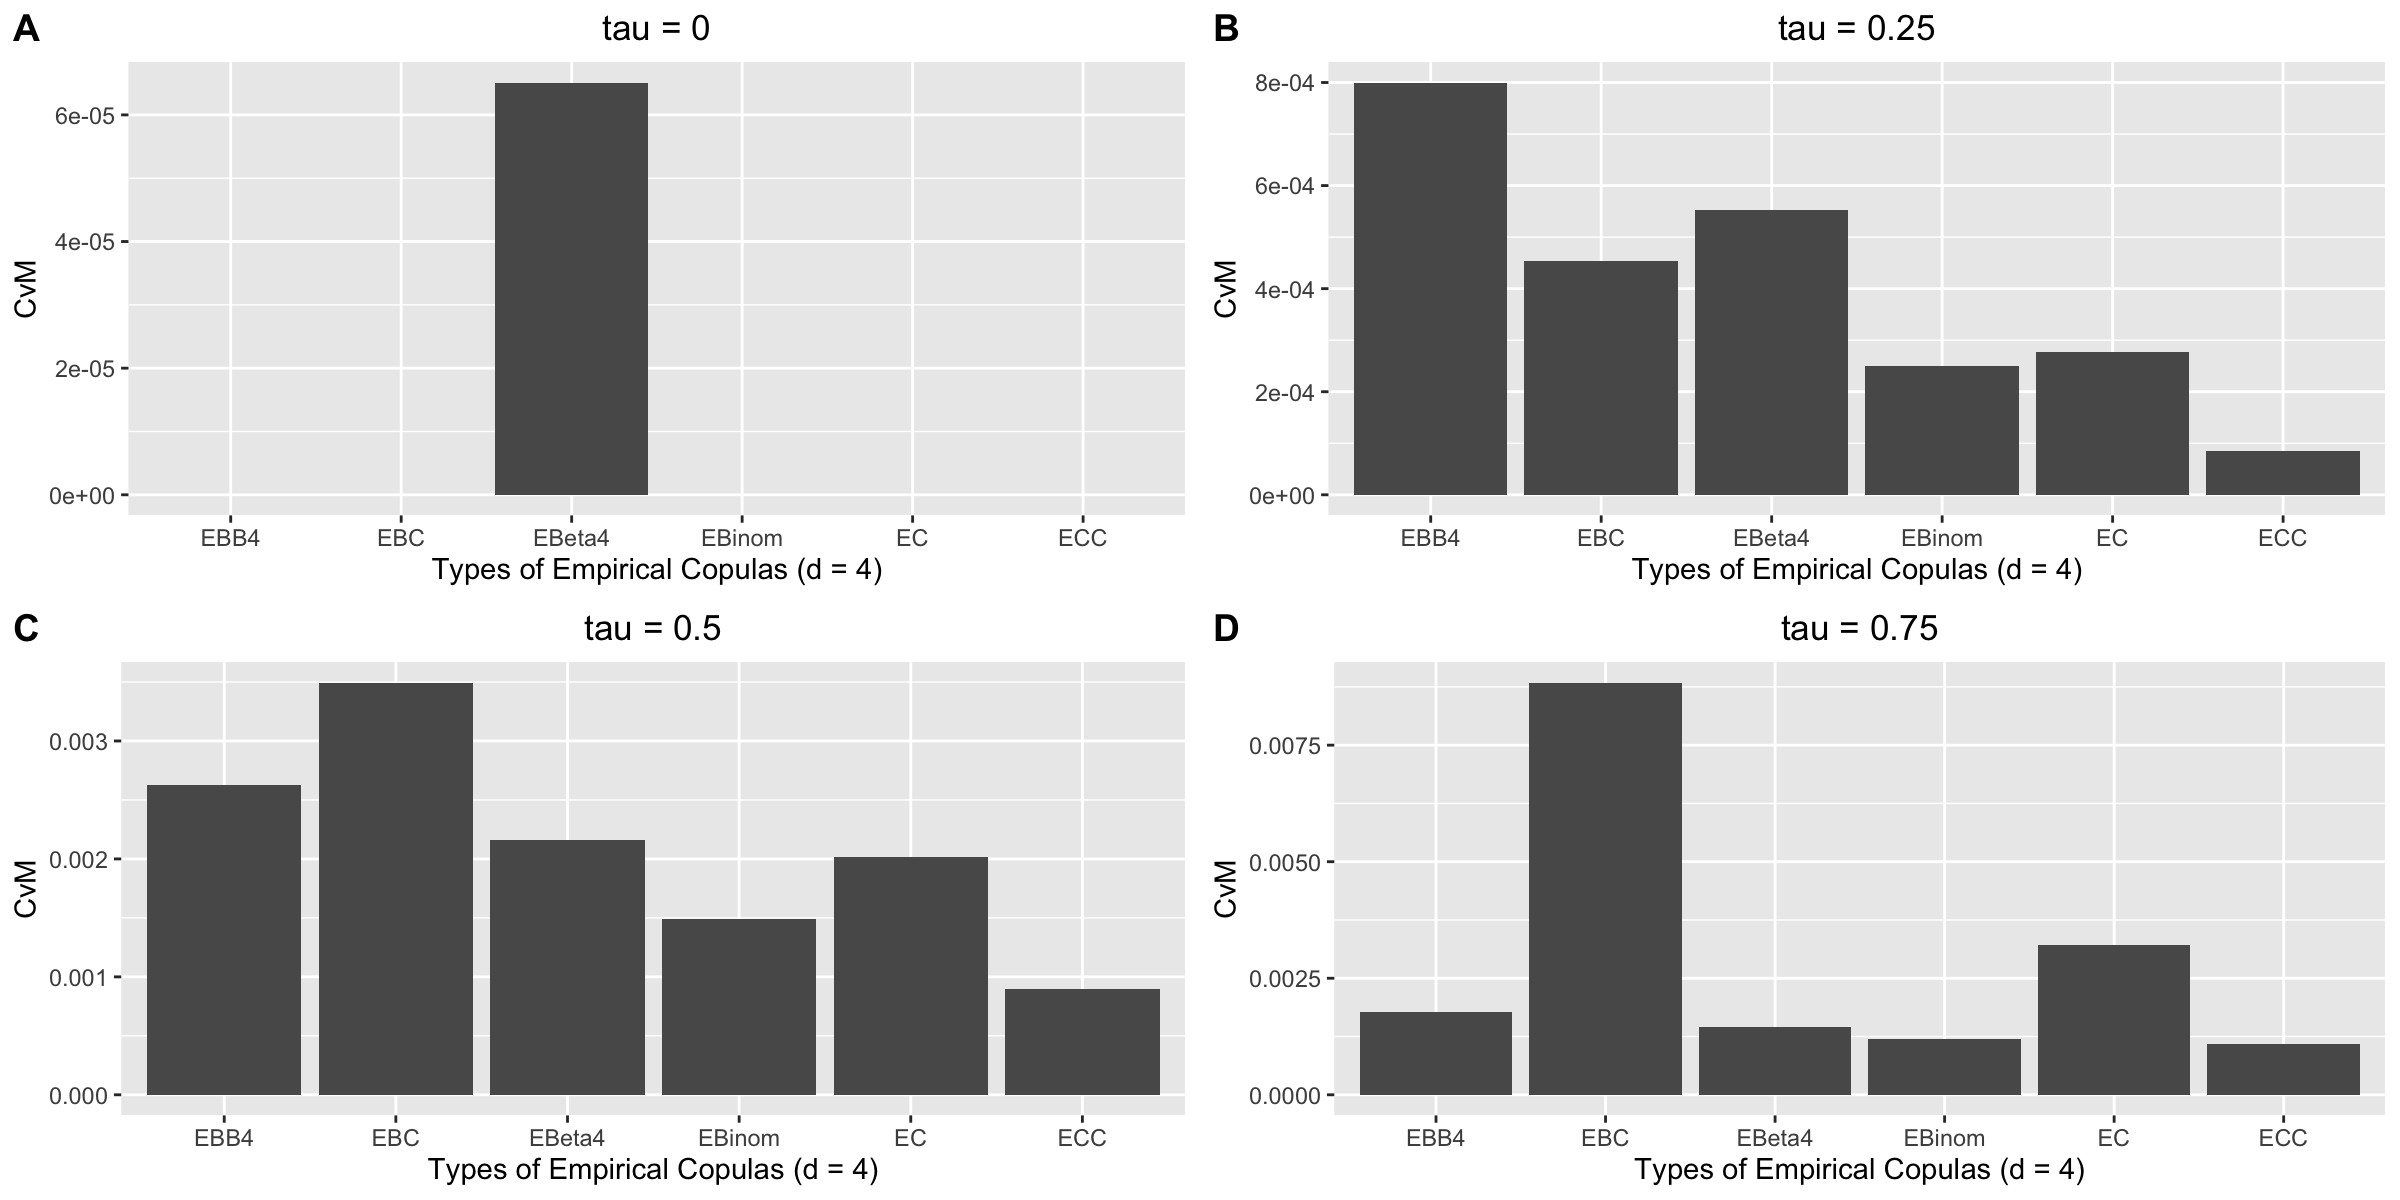
\includegraphics[width=17cm]{ExceedanceCvM/G_4d_s_CvM.png}
\captionof{figure}{Gumbel-Hougaard copula with $d$ = 4}
\end{center}%

\begin{center}
\label{G_5d_s_CvM}
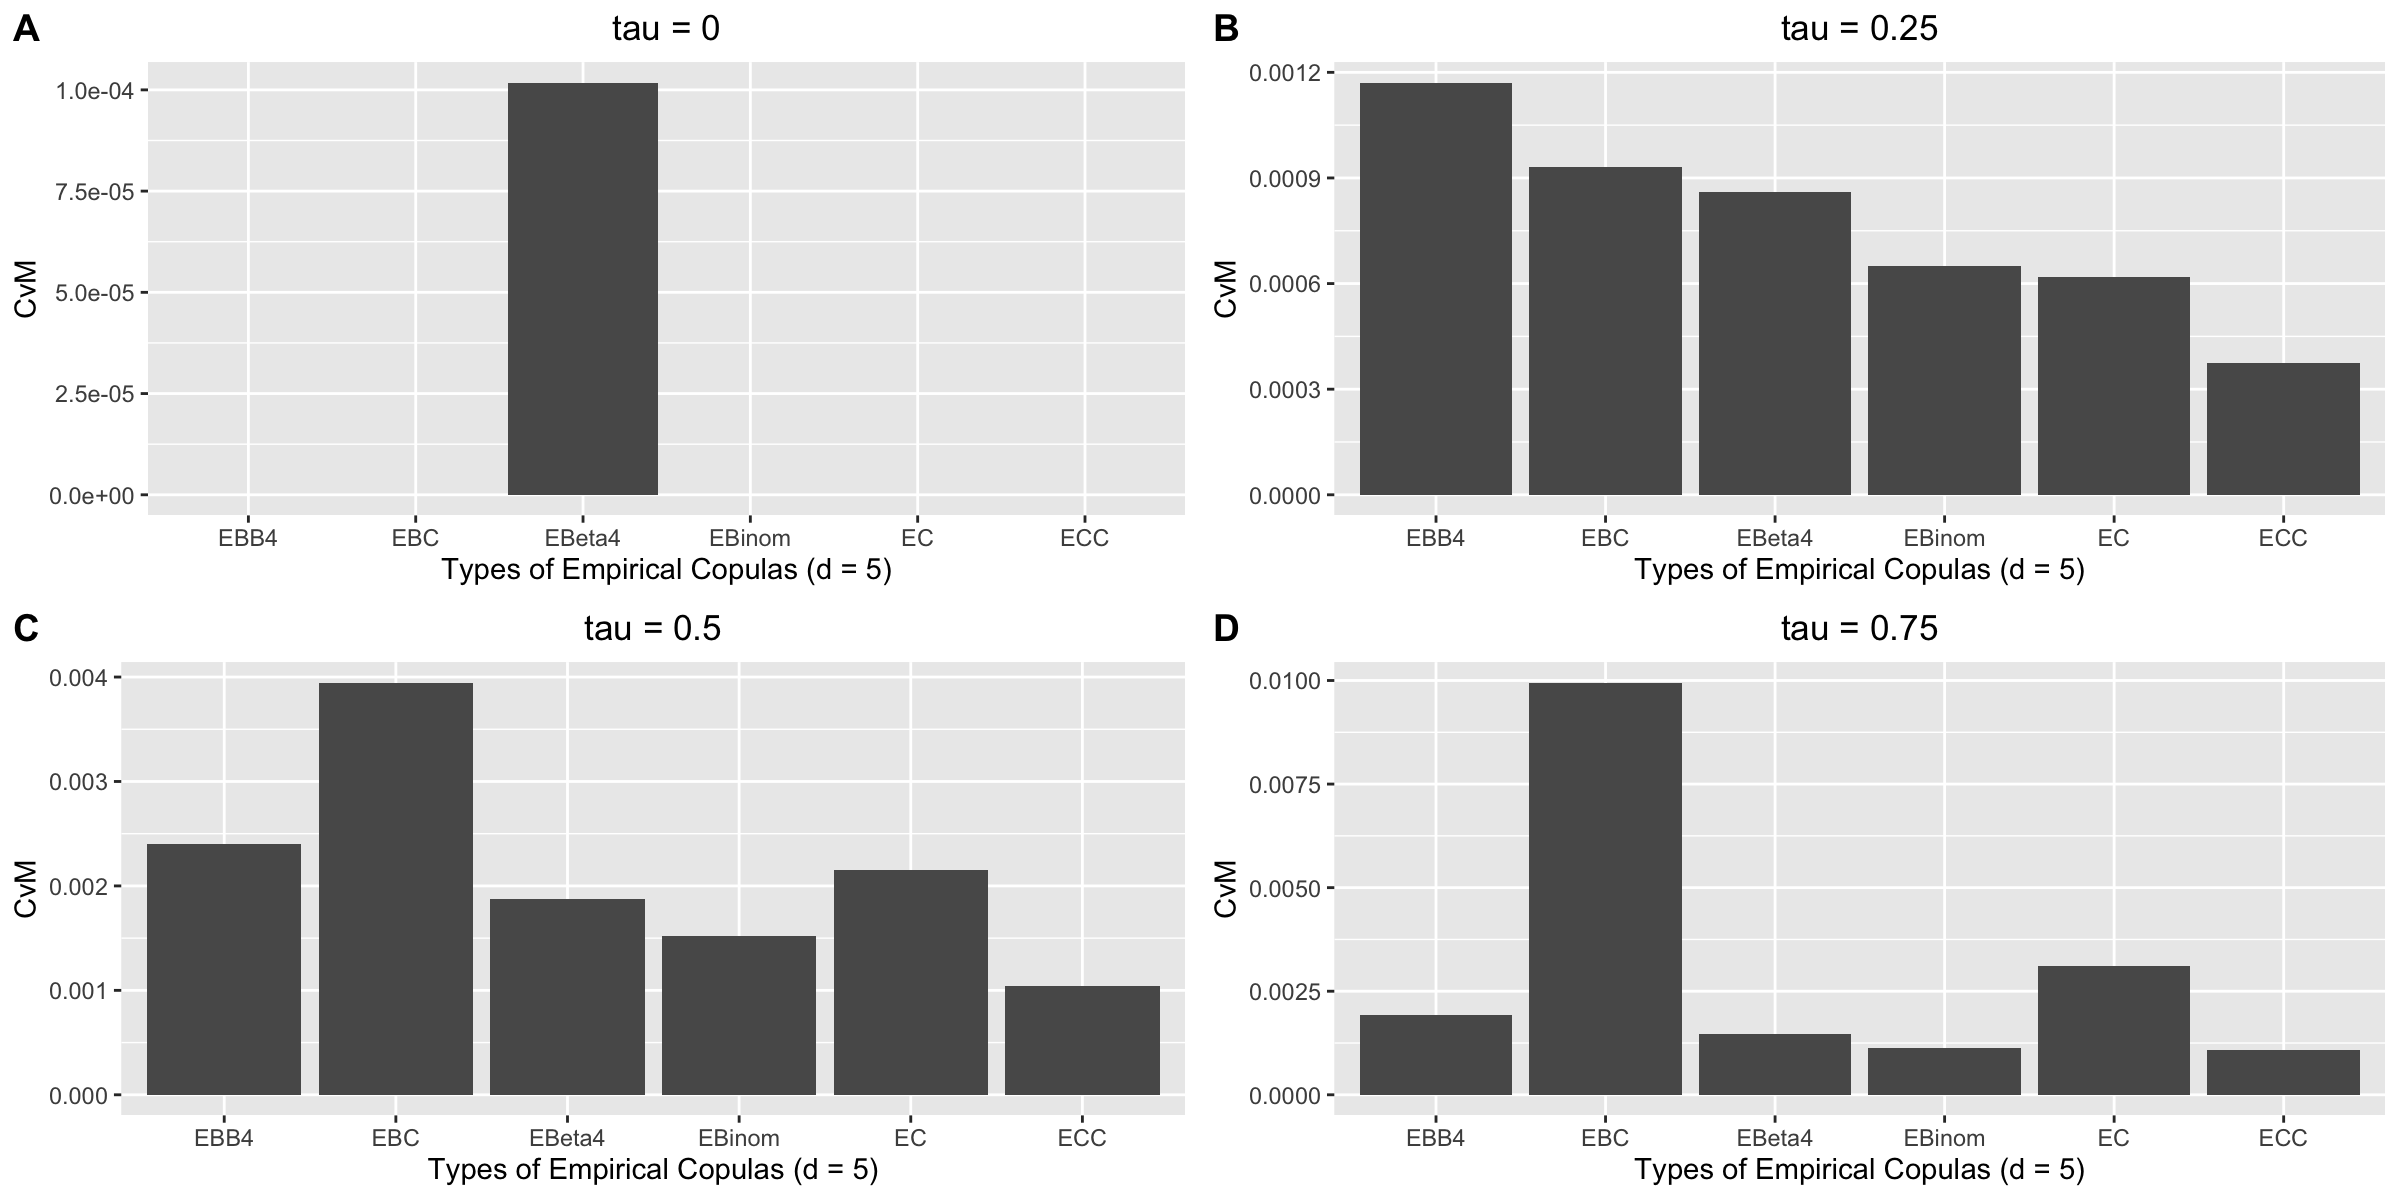
\includegraphics[width=17cm]{ExceedanceCvM/G_5d_s_CvM.png}
\captionof{figure}{Gumbel-Hougaard copula with $d$ = 5}
\end{center}%

\newpage
\subsection{Analysis: Exceedance probabilities}
\vspace{0.5cm}
There are a few conclusions that can be reached by analysing the aforementioned plots. \\

\subsubsection{Lower Kendall's tau values}
\vspace{0.5cm}
It can be observed that there are an overall worse predictive performance at the lower Kendall's tau (notably negative Kendall's tau). From intuition, a negative Kendall's tau represents that, in the bivariate case, the margins are negatively related (points are concentrated on the top-left or bottom-right corner). Similar intuition holds for high-dimensional cases. Hence, there is little-to-no weight on the lower-tail or upper-tail (i.e. in the bivariate case, bottom-left and top-right corner). In the current analysis, the size of the dataset is relatively small (i.e. $n = 125$). Hence, even when sampling 125 samples from the target true copula, it is unlikely that the sample created will have any weight at the upper tail. Hence, for a smaller tau, most copulas (except beta-survival margins smoothed empirical copula) vastly underestimate the upper tail. It is noted that some graphs show a systematic overestimation with respect to the true copula, which is intuitive; as the probability of having samples at the extreme tails (for small Kendall's tau values) is low, sampling differences might bring the estimated copula to underestimate or overestimate the true copula.\\
\vspace{0.5cm}
It is notable that the smoothed EBC-adapted empirical copula with beta-binomial survival margins seems to best estimate the true-copula at lower values of Kendall's tau, compared to the other two types of smoothed empirical copulas. \\
\vspace{0.5cm}
To more accurately estimate the true-copula by using empirical copulas, a larger $n$ is needed, as the class of empirical copula asymptotically converges to the true copula for large $n$. However, this becomes prohibitive when available data is not sufficient. 

\pagebreak
\subsubsection{Erratic behaviour from smoothed EBC-adapted empirical copula with beta survival margins}

It can be seen from the plots that the smoothed EBC-adapted empirical copula with beta survival margins has extremely volatile behaviour in the tail. It is noted that it is uncertain why the ``survival function" exhibits a non-monotone pattern, as it is likely to be caused by rounding errors at the edge, as the order of the exceedance probabilities are from negative 5 to 10. \\
\vspace{0.5cm}
However, it is still interesting to understand the reason why, unlike the other types of empirical copulas, there appears to be a hump near $u = 0.99$.\\
\vspace{0.5cm}
Recall that the smoothed EBC-adapted empirical copula with beta survival margins is defined as follows:
\begin{align*}
C_{n}^{v}(\boldsymbol{u}) &= \frac{1}{n} \sum\limits_{i = 1}^{n} C_{n}^{\beta} \left[\Bar{\mathcal{B}}_{u_{1}}^{\boldsymbol{X}}\left(\frac{R_{i,1} - 0.5}{n}\right), \dots, \Bar{\mathcal{B}}_{u_{d}}^{\boldsymbol{X}}\left(\frac{R_{i,d} - 0.5}{n}\right) \right]
\end{align*}
where $\Bar{\mathcal{B}}_{u_{j}}^{\boldsymbol{X}}$ is beta distributed. The survival function corresponding to this type of smoothed empirical copula is computed as follows:
\begin{align*}
\Bar{H}^{v}_{n}(\boldsymbol{u}) = \Bar{C}^{v}_{n}(\boldsymbol{1 -- u}) = \sum\limits_{J \subseteq \{1, \dots, d \} }(-1)^{|J|} C^{v}_{n} \left( u_{1}^{\mathds{1}(1\in J)}, \dots, u_{d}^{\mathds{1}(d\in J)} \right), \quad \boldsymbol{u} \in [0,1]^{d}
\end{align*}
Hence we can see the main influencing factor on the size of the survival function is the smoothed EBC-adapted empirical copula with dimensions $j \in \{1, \dots, d\}$. Note that the beta distribution defined above is distributed with scale parameters $\alpha$ and $\beta$: (proof by algebraic manipulation, and can be found in \cite{KojadinovicYi2024Smooth}):
\begin{align*}
\alpha &= \frac{n - \rho}{\rho} \times u_{j}, \: j \in \{1, \dots, d\} \\
\beta &= \frac{n - \rho}{\rho} \times (1 - u_{j}), \: j \in \{1, \dots, d\}
\end{align*}
In our simulation, we used $n = 125$ and $\rho = 4$, and $u_{j} \in \{0.95, \dots, 1\}$. The resulting range of $\alpha$ can be calculated as $\alpha \in [28.7375, 30.25]$, and the resulting range of $\beta$ can be calculated as $\beta \in [0, 1.5125]$. Hence, this is equivalent (componentwise), in evaluating the probability of a beta distribution with $\alpha \in [28.7375, 30.25]$ and $\beta \in [0, 1.5125]$ being larger than $\frac{R_{i,j} - 0.5}{n} \in (0,1)$. As the resulting $\alpha$ is extremely large and resulting $\beta$ is extremely small, this results in a extremely heavy-right-tailed beta distribution. Substituting into the smoothed empirical EBC-adapted empirical copula, it will result in a very abnormally large copula $C^{v}_{n} \left( u_{1}^{\mathds{1}(1\in J)}, \dots, u_{d}^{\mathds{1}(d\in J)} \right)$, and hence a peak in the exceedance probability. As the appearance of an ``up-tail" data point is rare during sampling, this sudden peak in the exceedance probability (in one data row) will skew the average exceedance probability. In further analysis, it is ideal to increase the sample size to see if this observations is retained.\\
\vspace{0.5cm}
With the following revelation, the smoothed EBC-adapted empirical copula with beta survival margins are very suitable (under a larger sample size n) to model extremal events (such as joint default scenarios).

\subsubsection{Systematic underestimation of the upper-tail at positive Kendall's tau}
By closely observing the plots for higher Kendall's tau (especially those with positive tau), we can observe that, albeit the estimators very closely resembles the true copula, it is often (systematically) lower than the true copula.\\
\vspace{0.5cm}
The problem of underestimation is rampant when the Kendall's tau is close to 0. Due to the relatively small sample size ($n = 125$) and the discretized nature of the empirical copula, it places 0 probability mass if all rows in $\boldsymbol{U}$ are smaller than the evaluation vector $\boldsymbol{u}$ (when computing the survival function of the empirical copula). In reality, the true copula still has weight on the upper tail (albeit negligible), hence leading to the underestimation of the copula. Similarly to the other types of empirical copulas, they are in a sense, just continuous versions (EBC / EBB4 / EBinom / EBeta4) / interpolations (ECC) of the empirical copula. Hence, this underestimation property is unfortunately unavoidable, and could be overcame by increasing the sample size (as they are asymptotically convergent). As mentioned in the previous section, it is often unrealistic. 

\subsubsection{Bias and variance of different empirical estimators}
From a interpretation standpoint, the empirical copula and the empirical beta copula are most ``interpretable" in the sense that these two empirical copulas' sampling algorithms are most simplistic, hence by interpreting the plots, it is easy to understand the result, in whether they are reasonable and intuitive. However, this is not the main focus of this work. We try to understand the bias and variance of the estimator with respect to the true copula in the following paragraphs.\\ 
\vspace{0.5cm}
From a bias standpoint, we can try to interpret the Cramer-von-Mises statistic. It is possible, under a parametric setup, to estimate the p-value associated with the Cramer-von-Mises statistic. However, as the use of the class of empirical copulas is nonparametric, it is not possible to estimate the p-value of the Cramer-von-Mises statistic. Moreover, as we are utilising pseudo-observations, it is not suitable to devise a hypothesis test (and compute p-values). Hence, we will understand the proximity of the estimator to the true copula by comparing the magnitude of the CvM statistic between the different estimators.\\
\vspace{0.5cm}
For low values of Kendall's tau (non-positive tau), we can observe that the overall best performing estimator is the smoothed EBC-adapted empirical copula with beta-binomial survival margins, with the smallest $S^{CvM}_{n}$ for most Kendall's tau $\le$ 0 (with the exception of student-$t$ $d$ = 2 and $\tau$ = $\{-0.5, 0\})$. However, the smoothed EBC-adapted empircal copula with beta survival margins is the worse performing estimator, as it has a much higher CvM compared to the other estimators (due to the erratic tail mentioned in previous sections).\\
\vspace{0.5cm}
For higher values of Kendall's tau (especially positive tau), we can observe that the empirical checkerboard copula and the 3 smoothed empirical copulas proposed by \cite{KojadinovicYi2024Smooth} overperforms the empirical copula and the empirical beta copula, as the CvM statistic is vastly smaller than EBC and EC (with some exceptions). Remarkably, the EBC-adapted empirical copula with binomial margins is the best performing estimator at high values of Kendall's tau with only few exceptions.\\
\vspace{0.5cm}
For the variance of the empirical copulas with respect to the real copula, we have also shown the confidence intervals implied by each empirical copula (in dotted lines). It can be remarked that the smoothed EBC-adapted empirical copula with beta-binomial and binomial survival margins respectively, have the lowest variance compared to the other estimators. This shows that beta-binomial and binomial survival margins smoothed EBC-adapted copula can achieve similar stability compared to other types of empirical copula even with a smaller sample size, which makes it a good candidate for tail modelling. On the other hand, despite the empirical checkerboard copula's exceedingly low bias (due to its interpolative nature), the variance is higher than the other empirical copulas. It can be understood as the fact that empirical checkerboard copulas is an interpolation of the empirical copula, it is extremely flexible (in the bias-variance trade-off sense) and hence is prone to high variation, hence the higher variance.\\
\vspace{0.5cm}
It is important to note that there is no adequate estimators for negative values of Kendall's tau for this sample size. \\

\newpage
\subsection{Plots: $\textbf{u}$ (evaluation points) vs cumulative probabilities}
\vspace{0.5cm}
We then plot the (lower-tailed) evaluation points against the cumulative probabilities for each empirical copula. The evaluation points are on the x-axis and the cumulative probabilities are on the y-axis. The solid line is the mean of the exceedance probabilities corresponding to the evaluation point, and the dotted line is the confidence intervals of the exceedance probabilities corresponding to the evaluation point.

\begin{center}
\label{t4_2d_c}
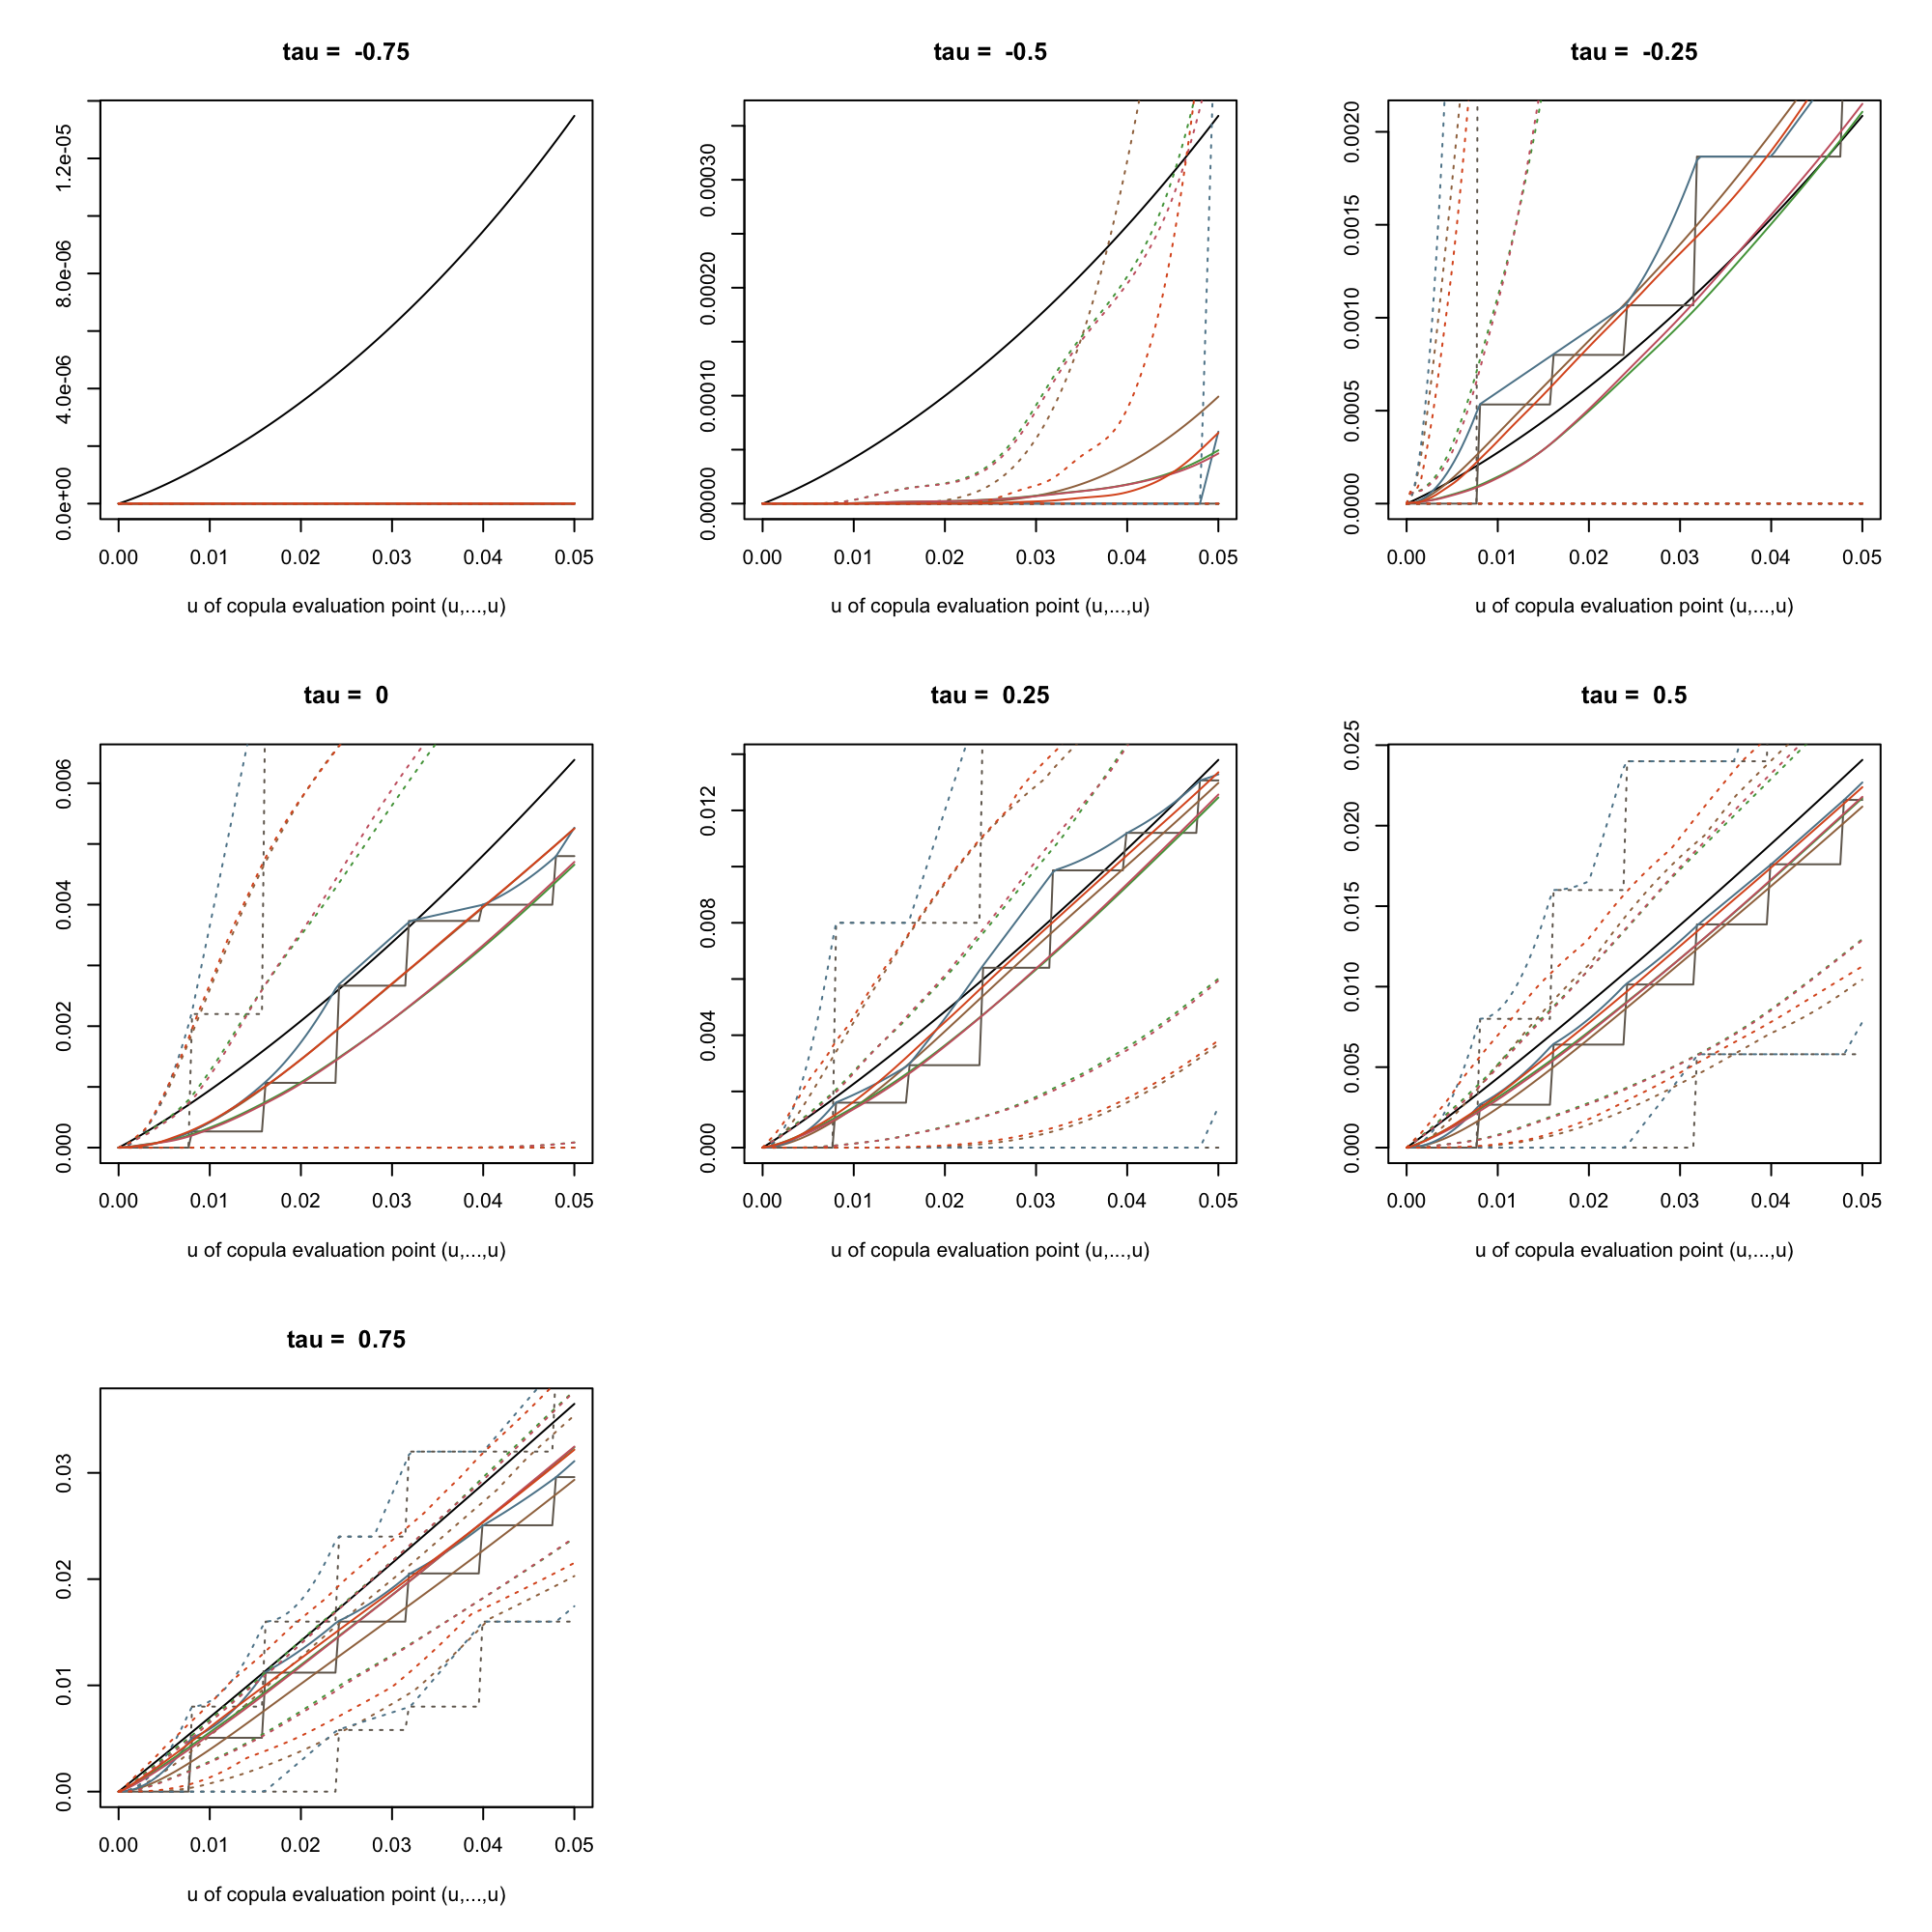
\includegraphics[width=17cm]{CumulativeProb/t4_2d_c.png}
\captionof{figure}{Student-$t$ copula with $d$ = 2}
\end{center}%

\begin{center}
\label{N_2d_c}
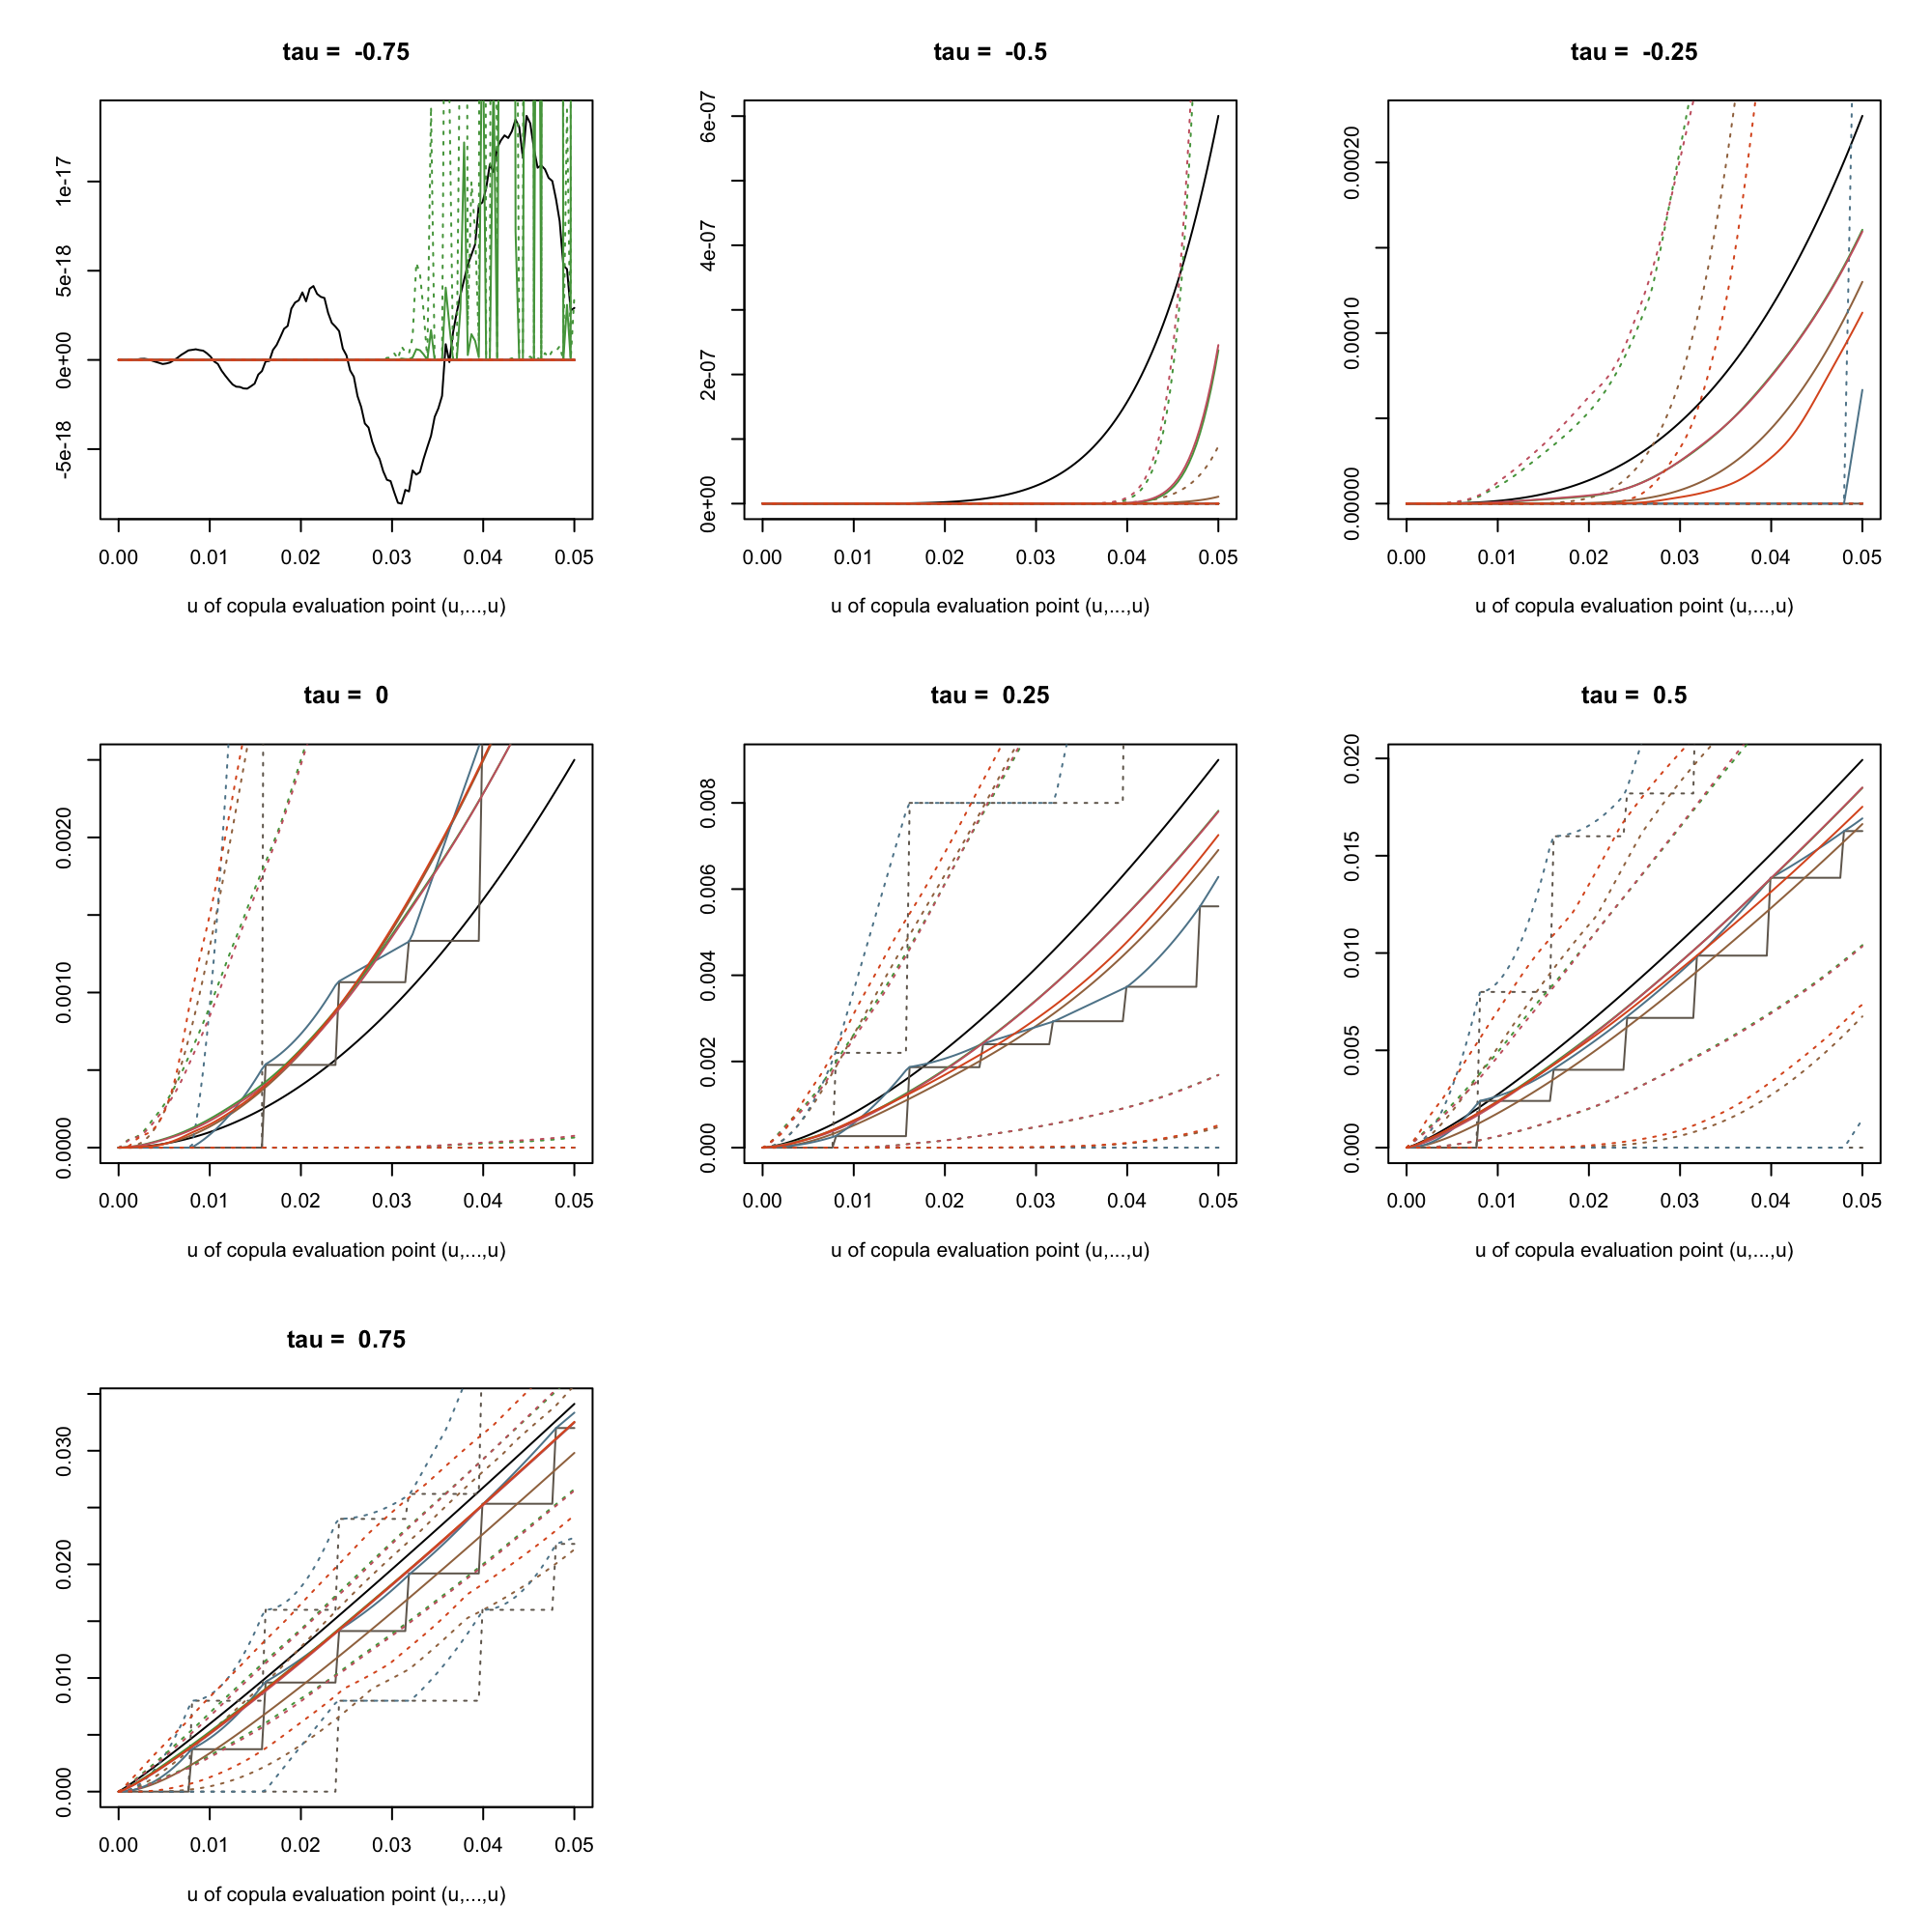
\includegraphics[width=17cm]{CumulativeProb/N_2d_c.png}
\captionof{figure}{Gaussian copula with $d$ = 2}
\end{center}%

\begin{center}
\label{C_2d_c}
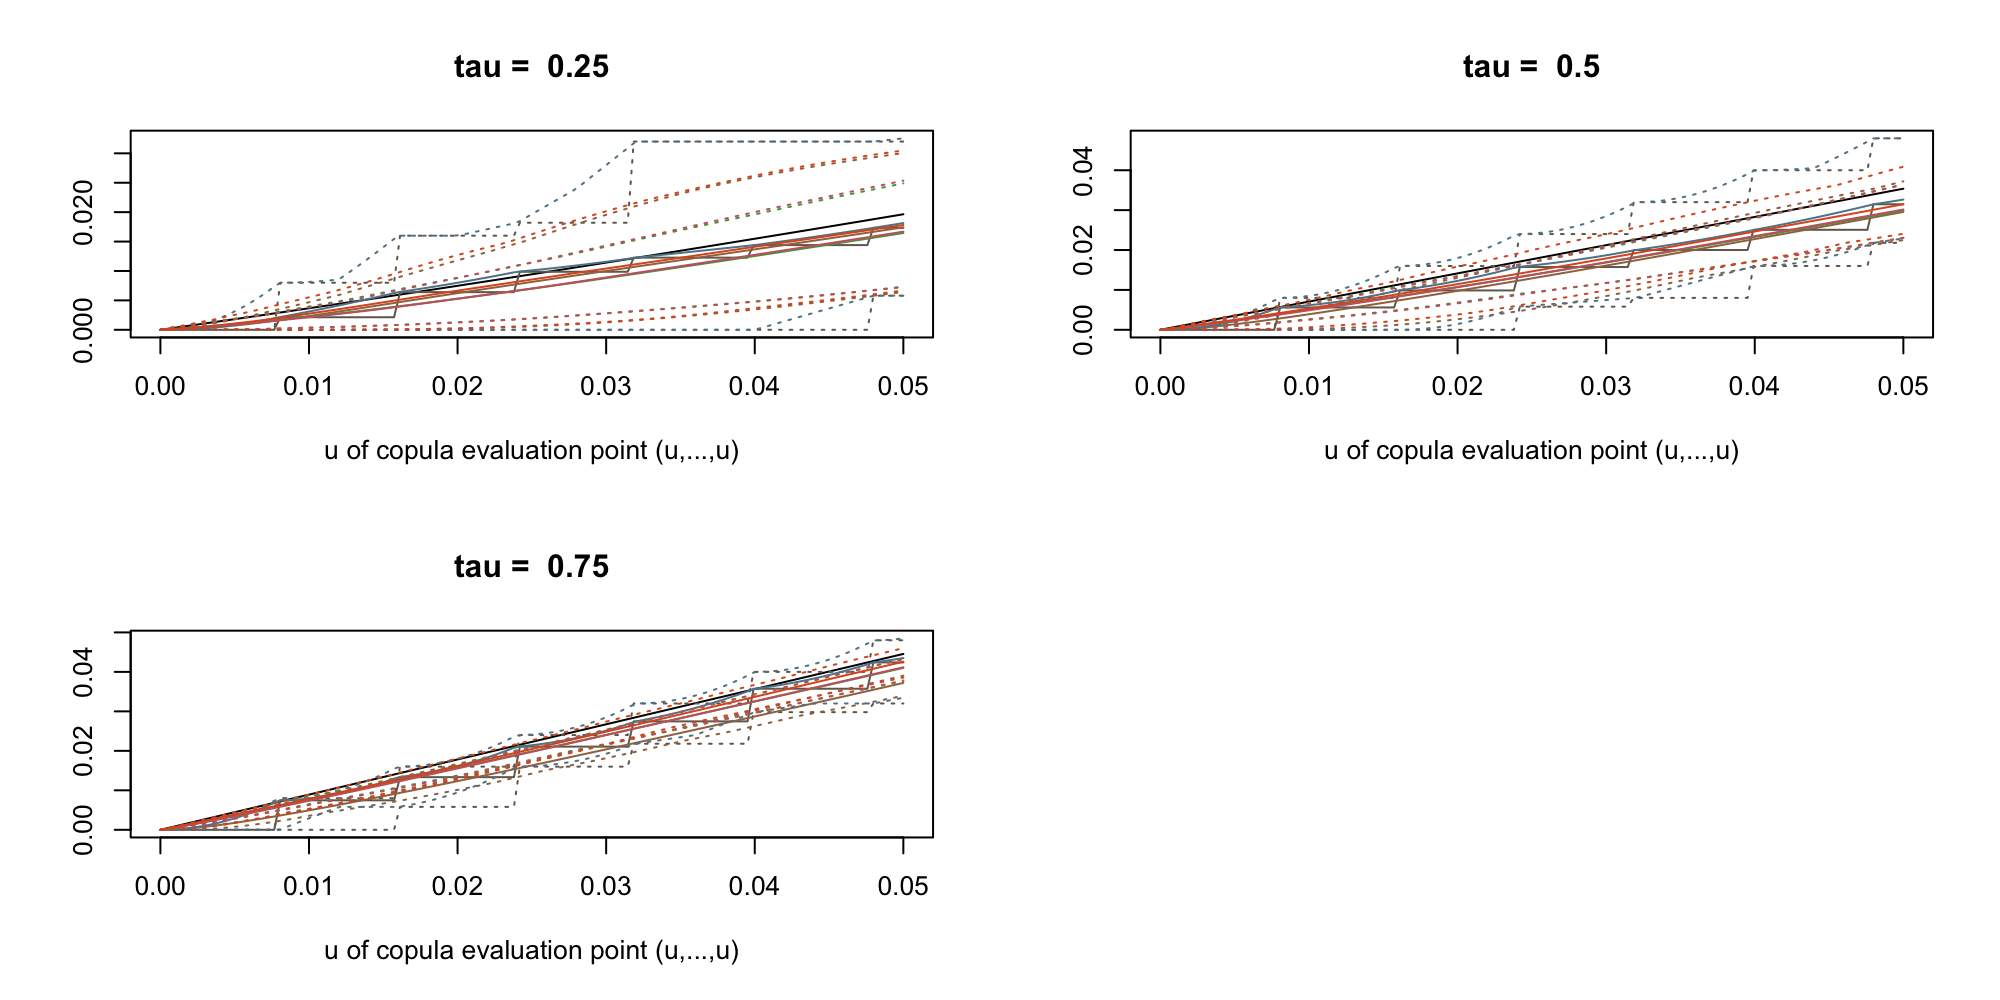
\includegraphics[width=17cm]{CumulativeProb/C_2d_c.png}
\captionof{figure}{Clayton copula with $d$ = 2}
\end{center}%

\begin{center}
\label{C_3d_c}
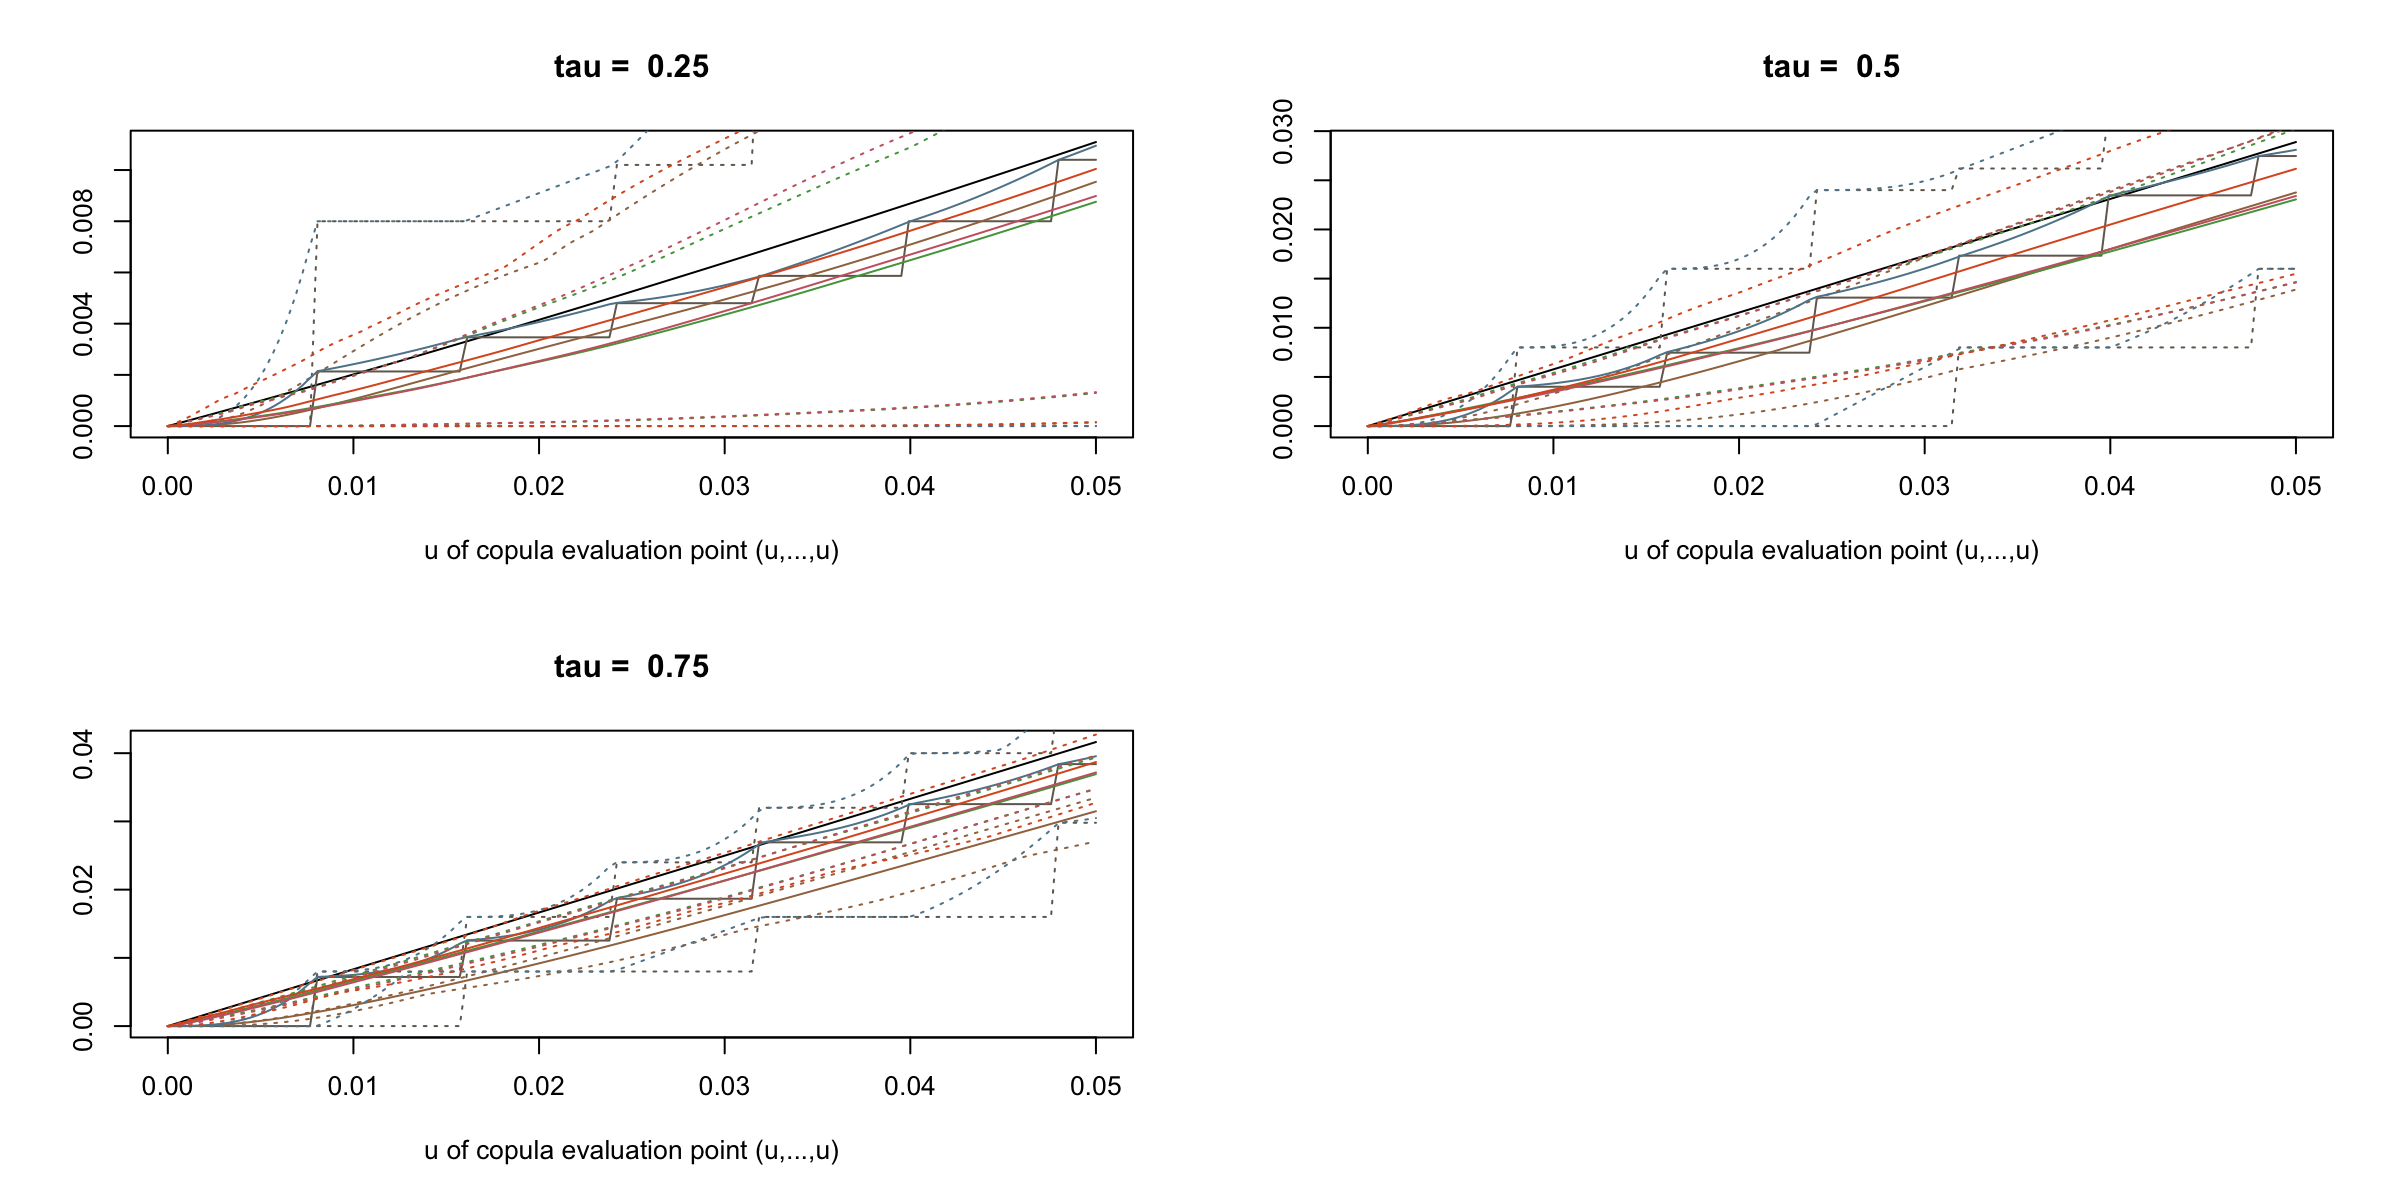
\includegraphics[width=17cm]{CumulativeProb/C_3d_c.png}
\captionof{figure}{Clayton copula with $d$ = 3}
\end{center}%

\begin{center}
\label{C_4d_c}
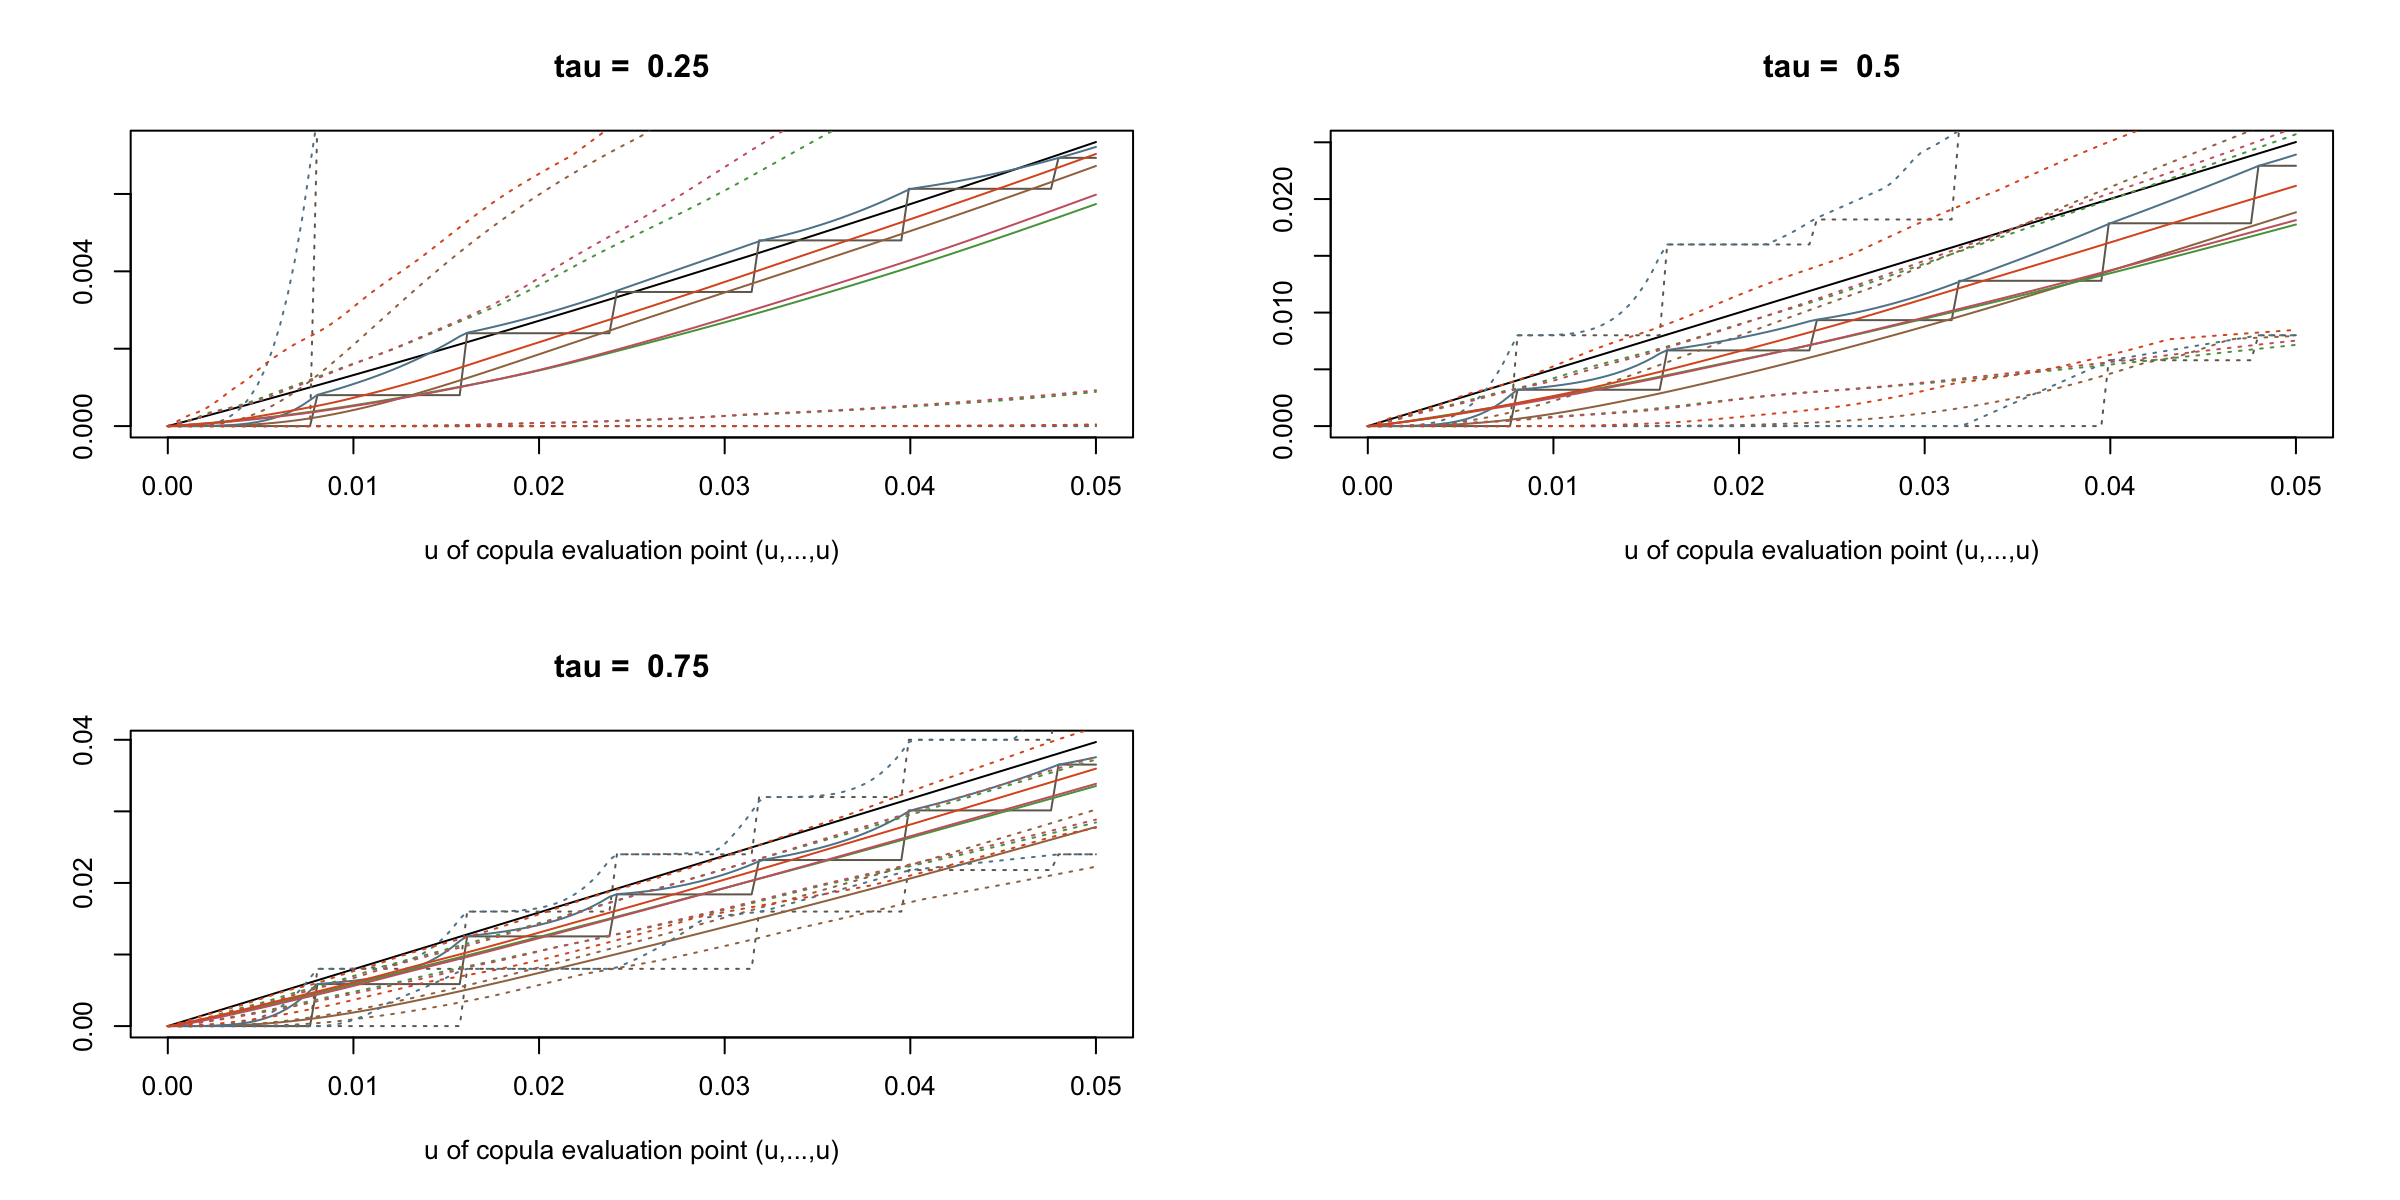
\includegraphics[width=17cm]{CumulativeProb/C_4d_c.png}
\captionof{figure}{Clayton copula with $d$ = 4}
\end{center}%

\begin{center}
\label{C_5d_c}
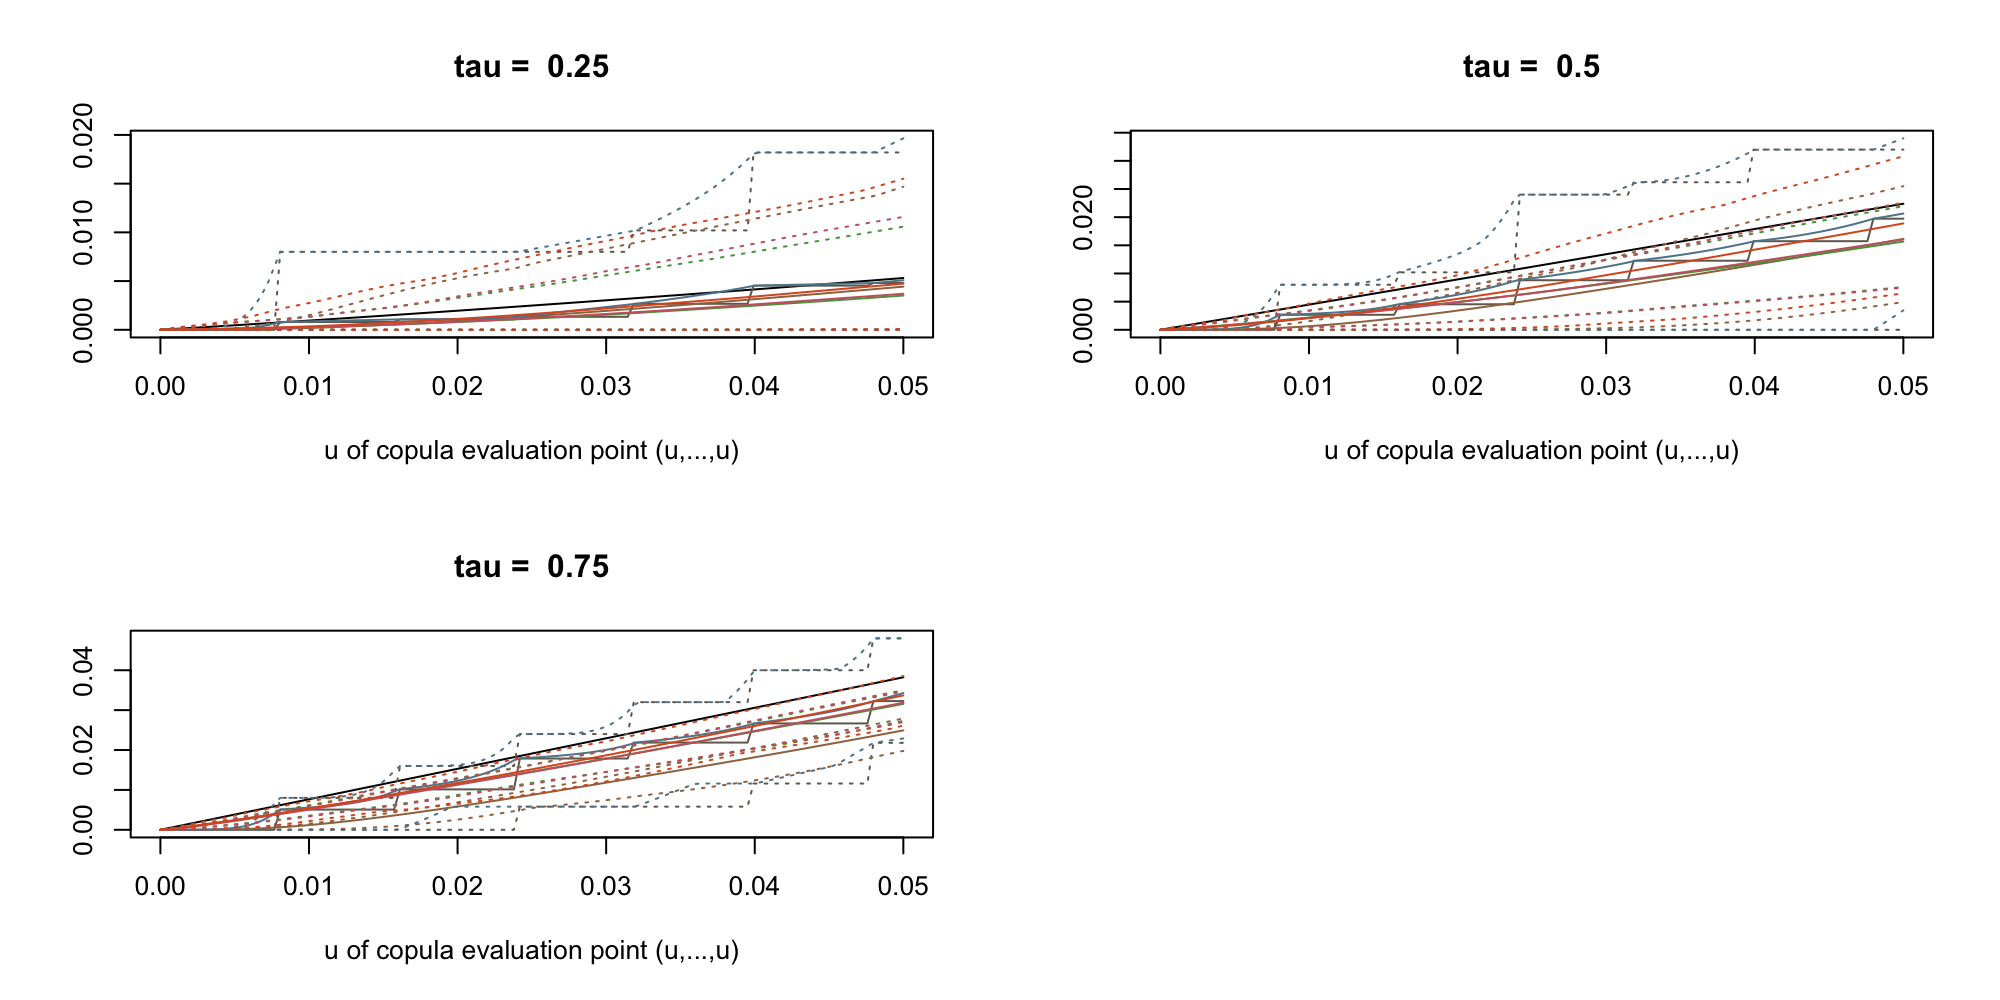
\includegraphics[width=17cm]{CumulativeProb/C_5d_c.png}
\captionof{figure}{Clayton copula with $d$ = 5}
\end{center}%


\newpage
\subsection{CvM: Cumulative probabilities}
To better understand the proximity of the cumulative probabilities for the class of empirical copula, with respect to the true copula, we then compute the Cramer-von-Mises statistics for all combinations of empirical copulas, Kendall's tau and dimensions.

\begin{center}
\label{t4_2d_c_CvM}
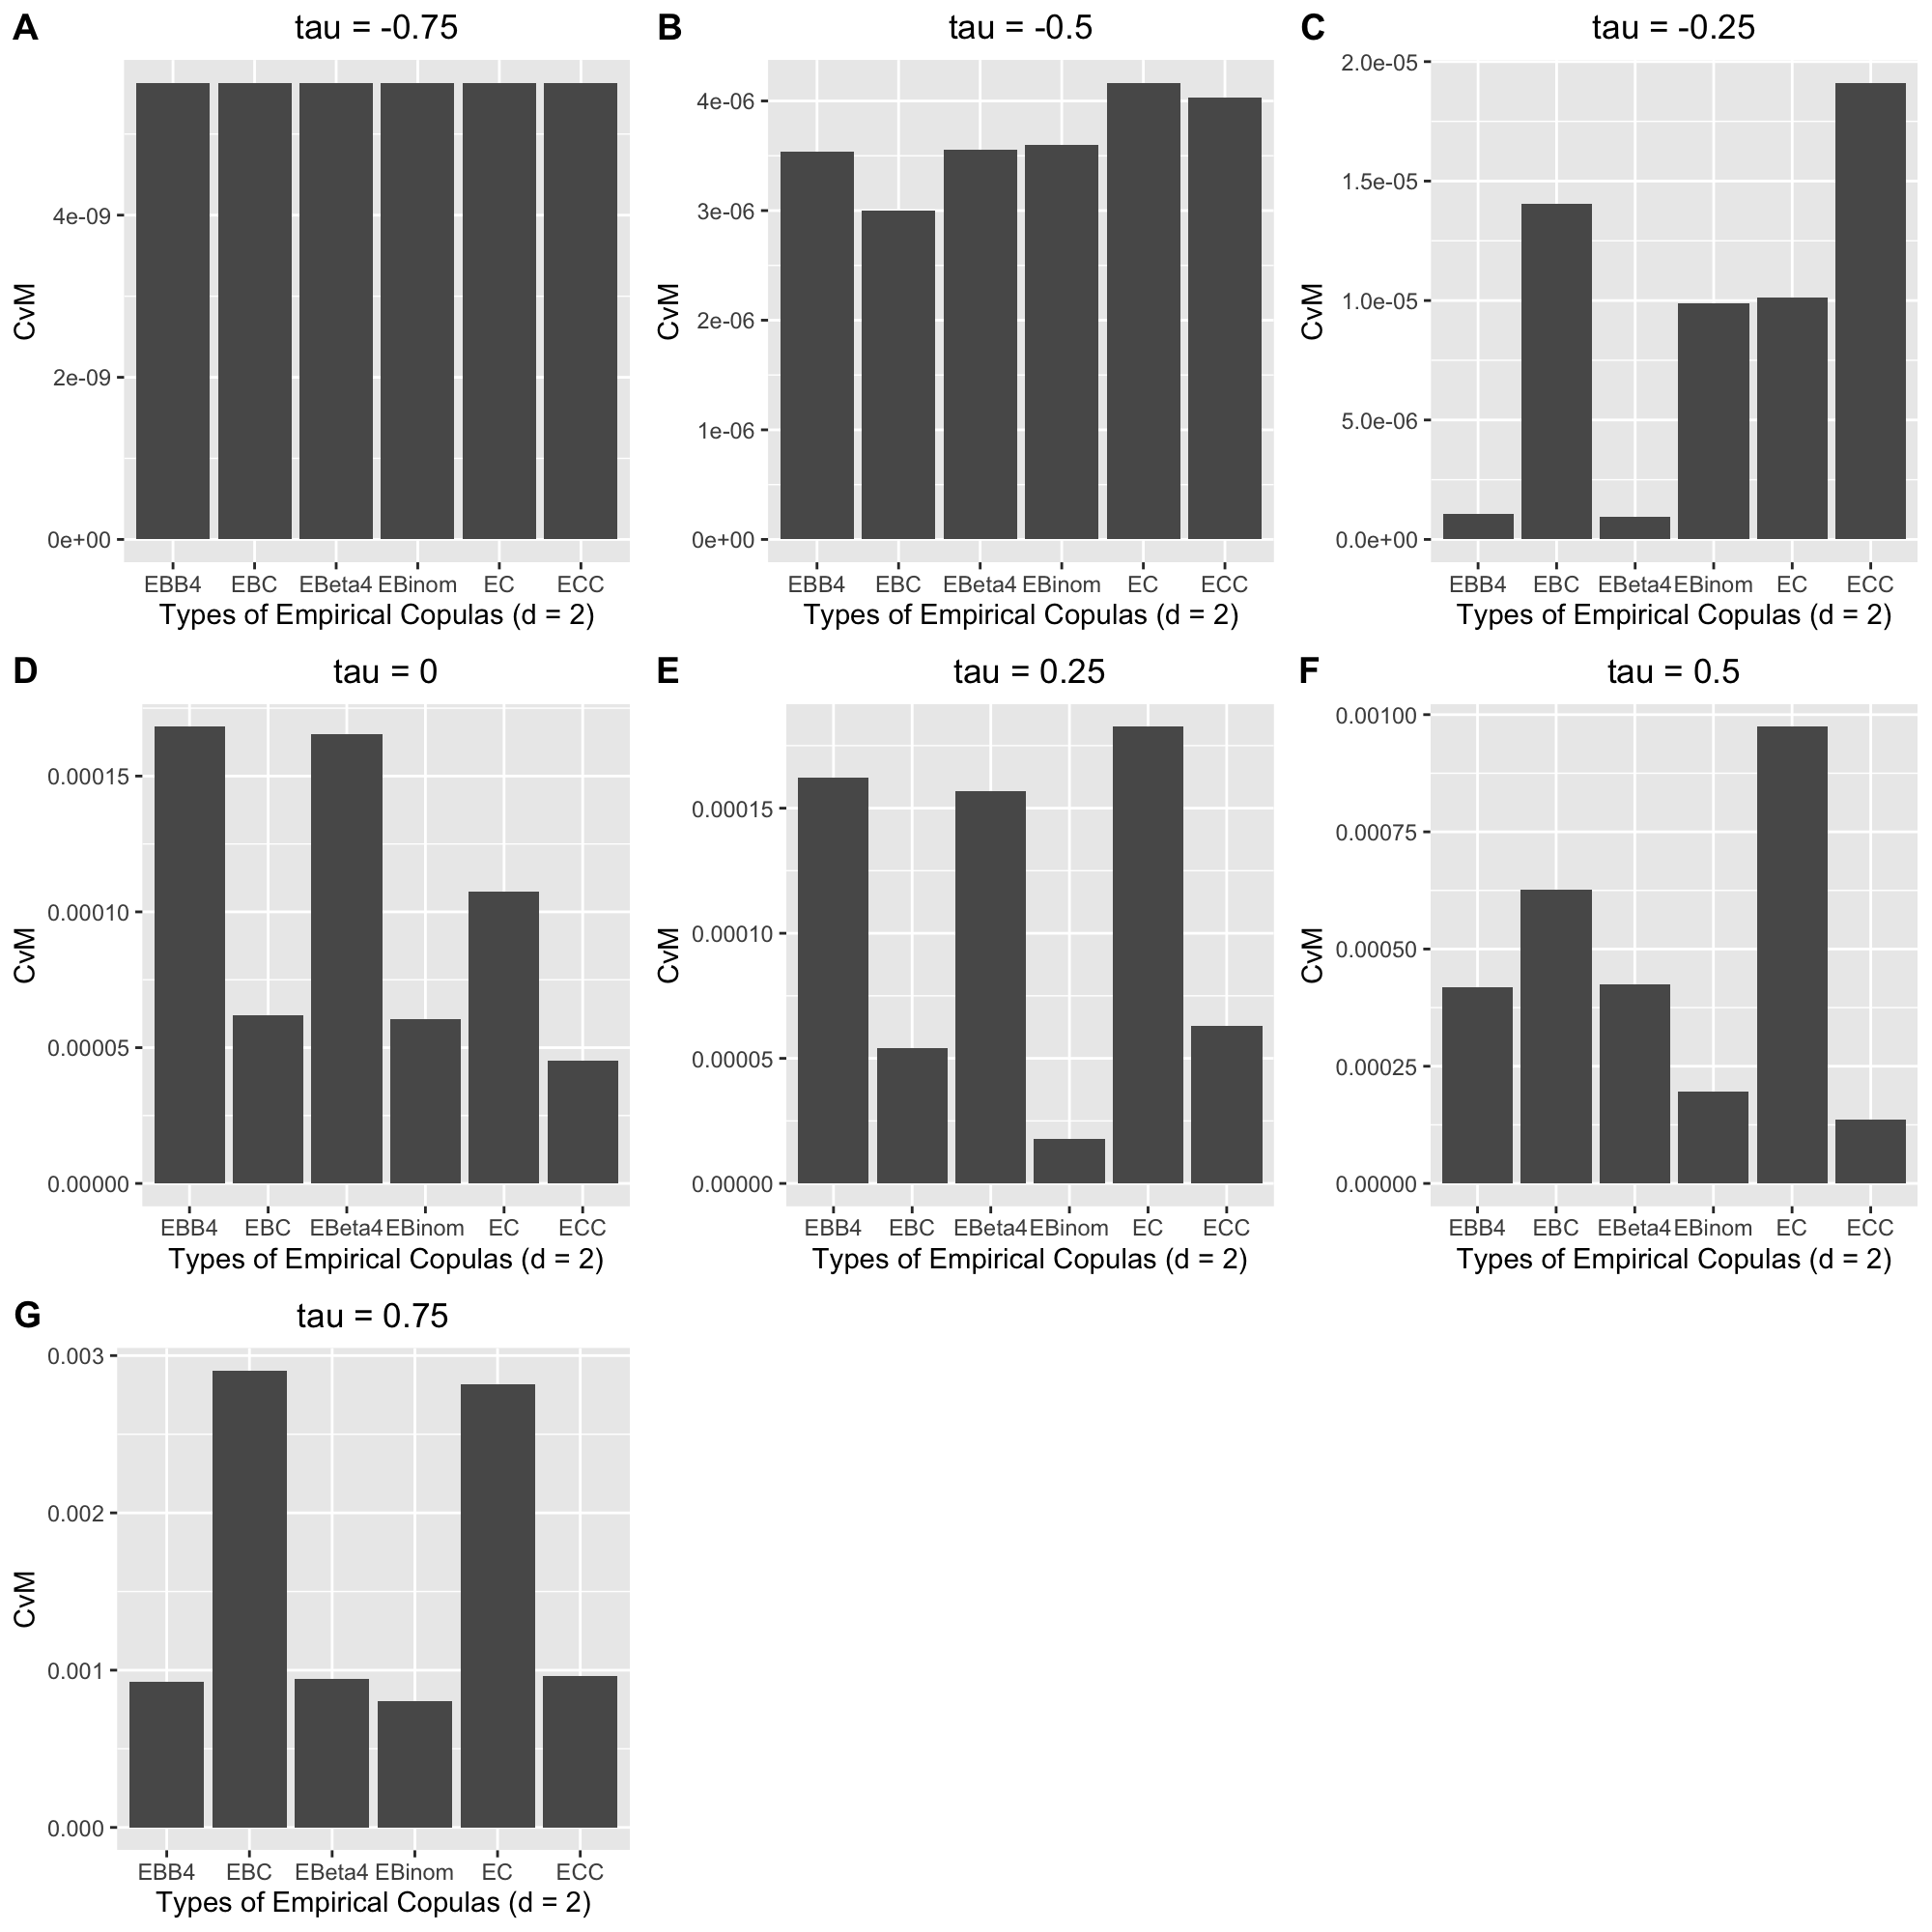
\includegraphics[width=17cm]{CumulativeCvM/t4_2d_c_CvM.png}
\captionof{figure}{Student-$t$ copula with $d$ = 2}
\end{center}%

\begin{center}
\label{N_2d_c_CvM}
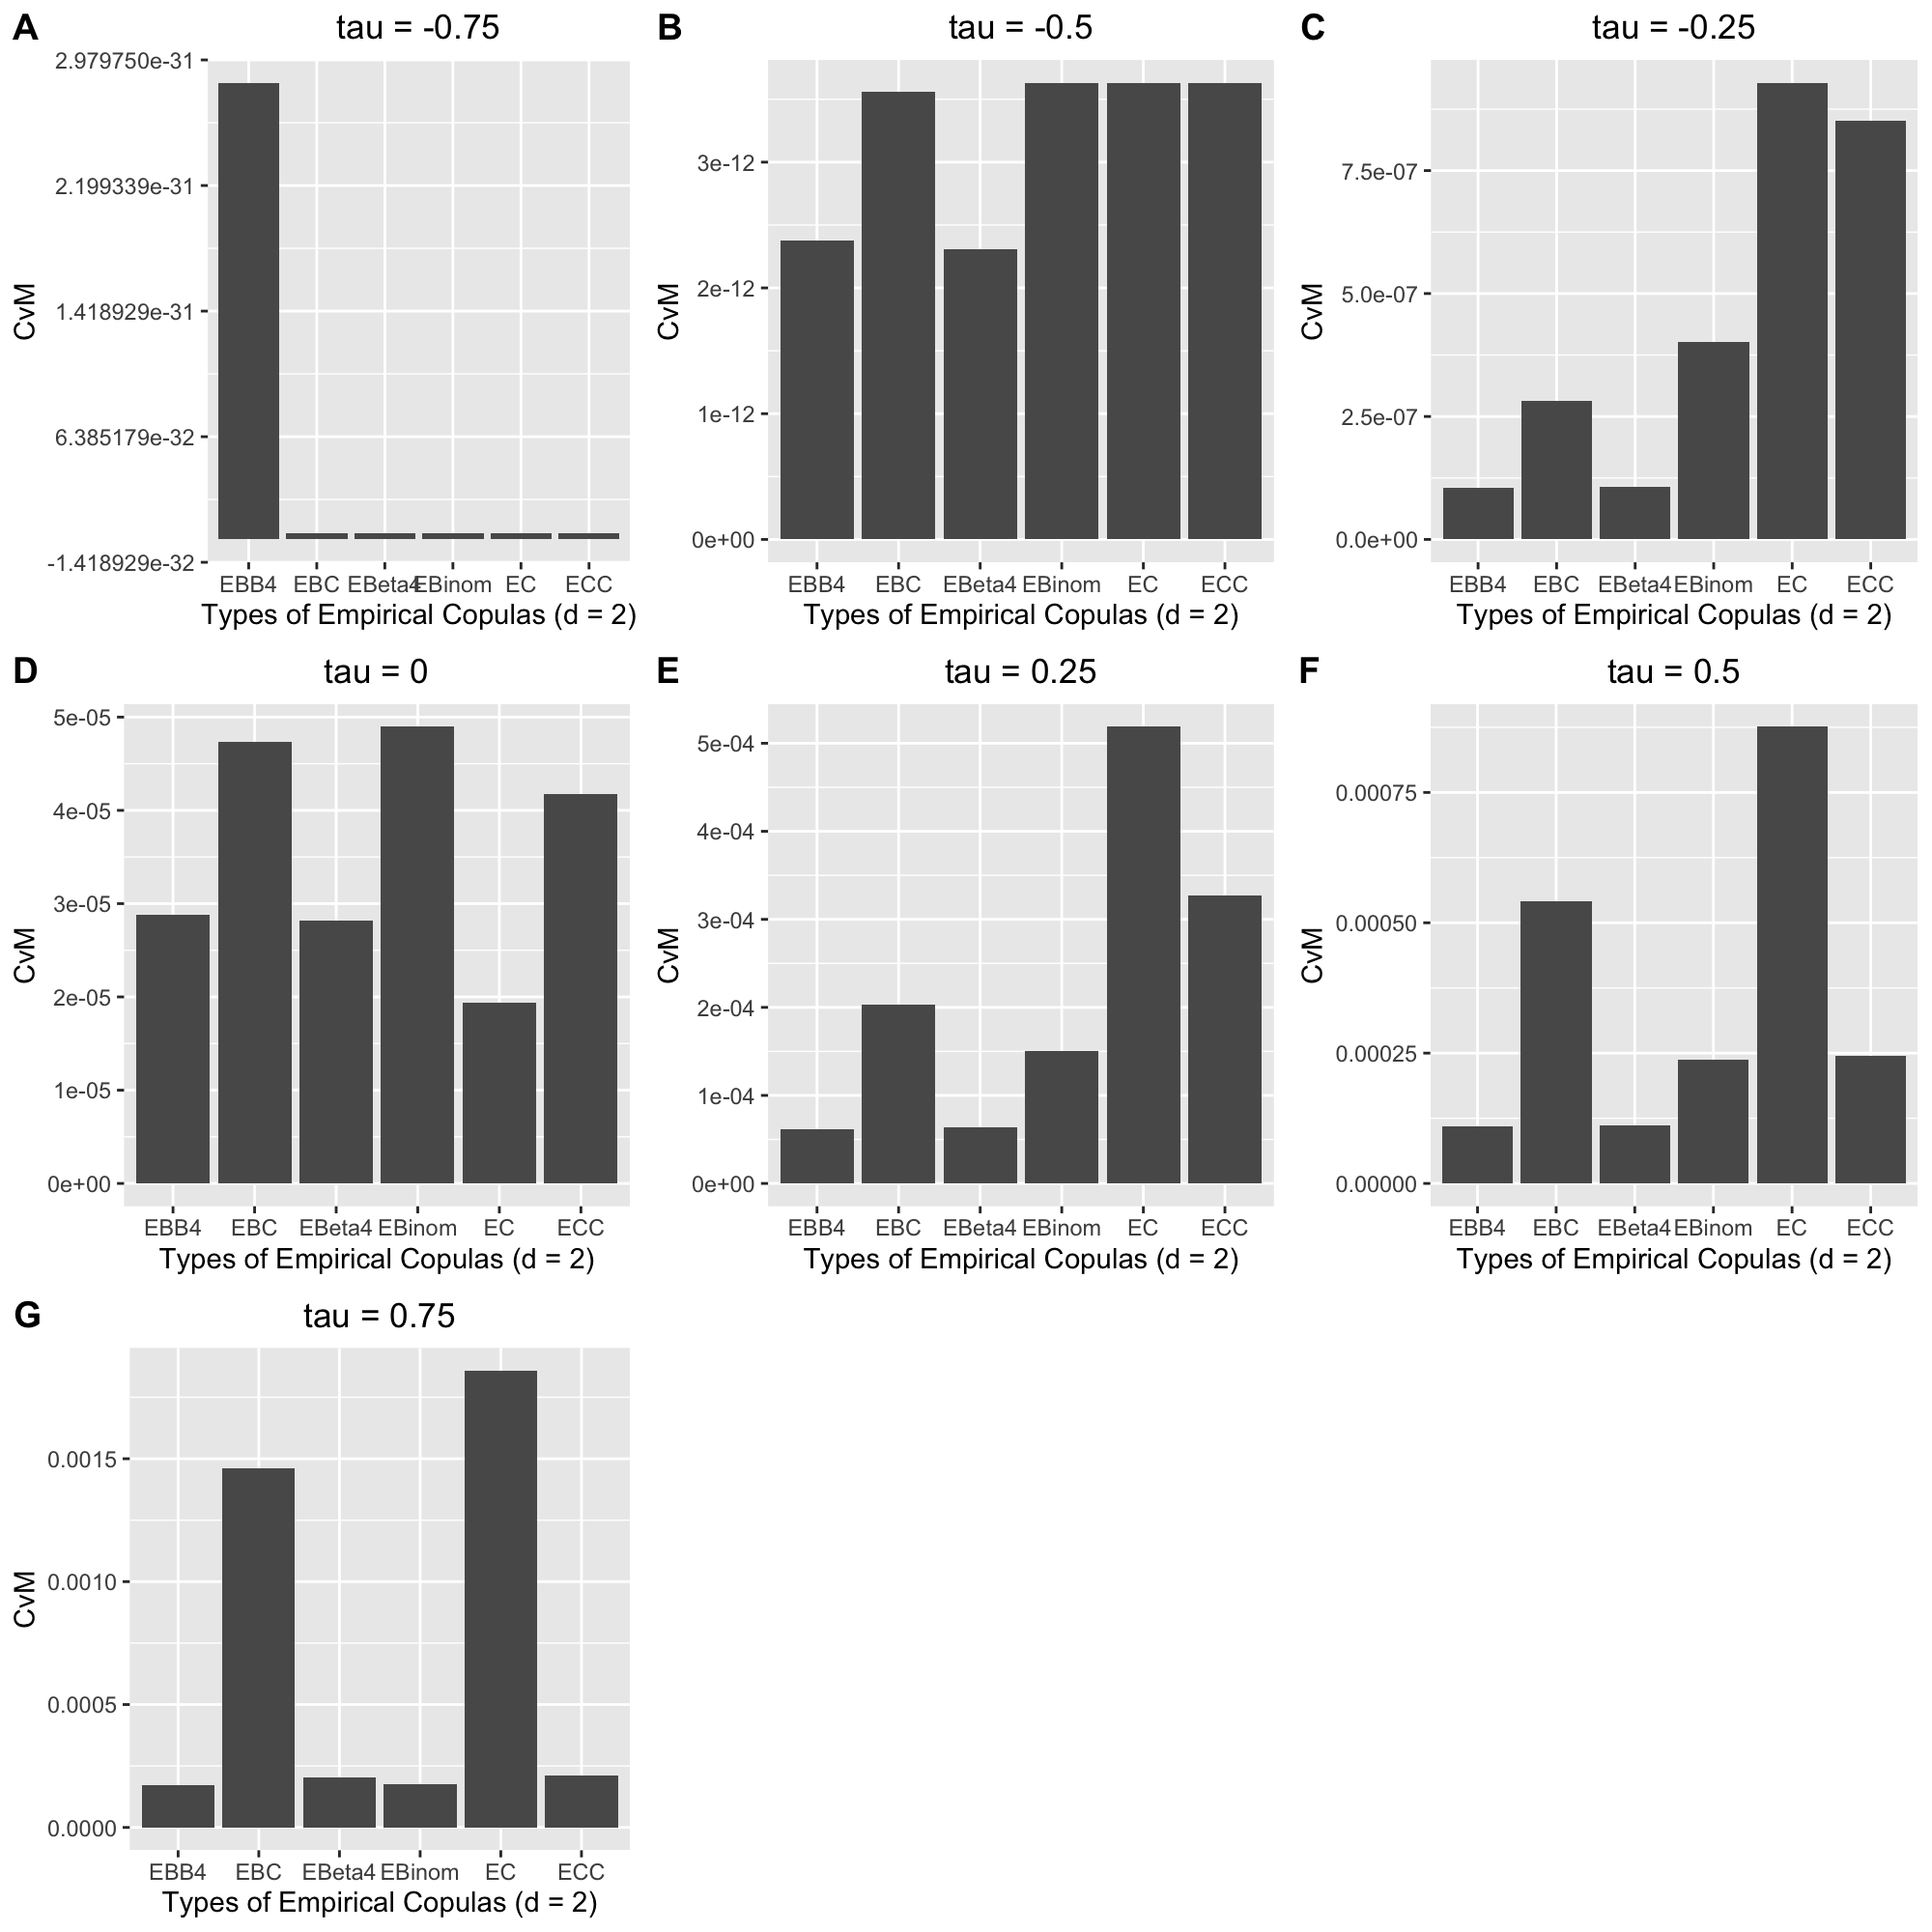
\includegraphics[width=17cm]{CumulativeCvM/N_2d_c_CvM.png}
\captionof{figure}{Gaussian copula with $d$ = 2}
\end{center}%

\begin{center}
\label{C_2d_c_CvM}
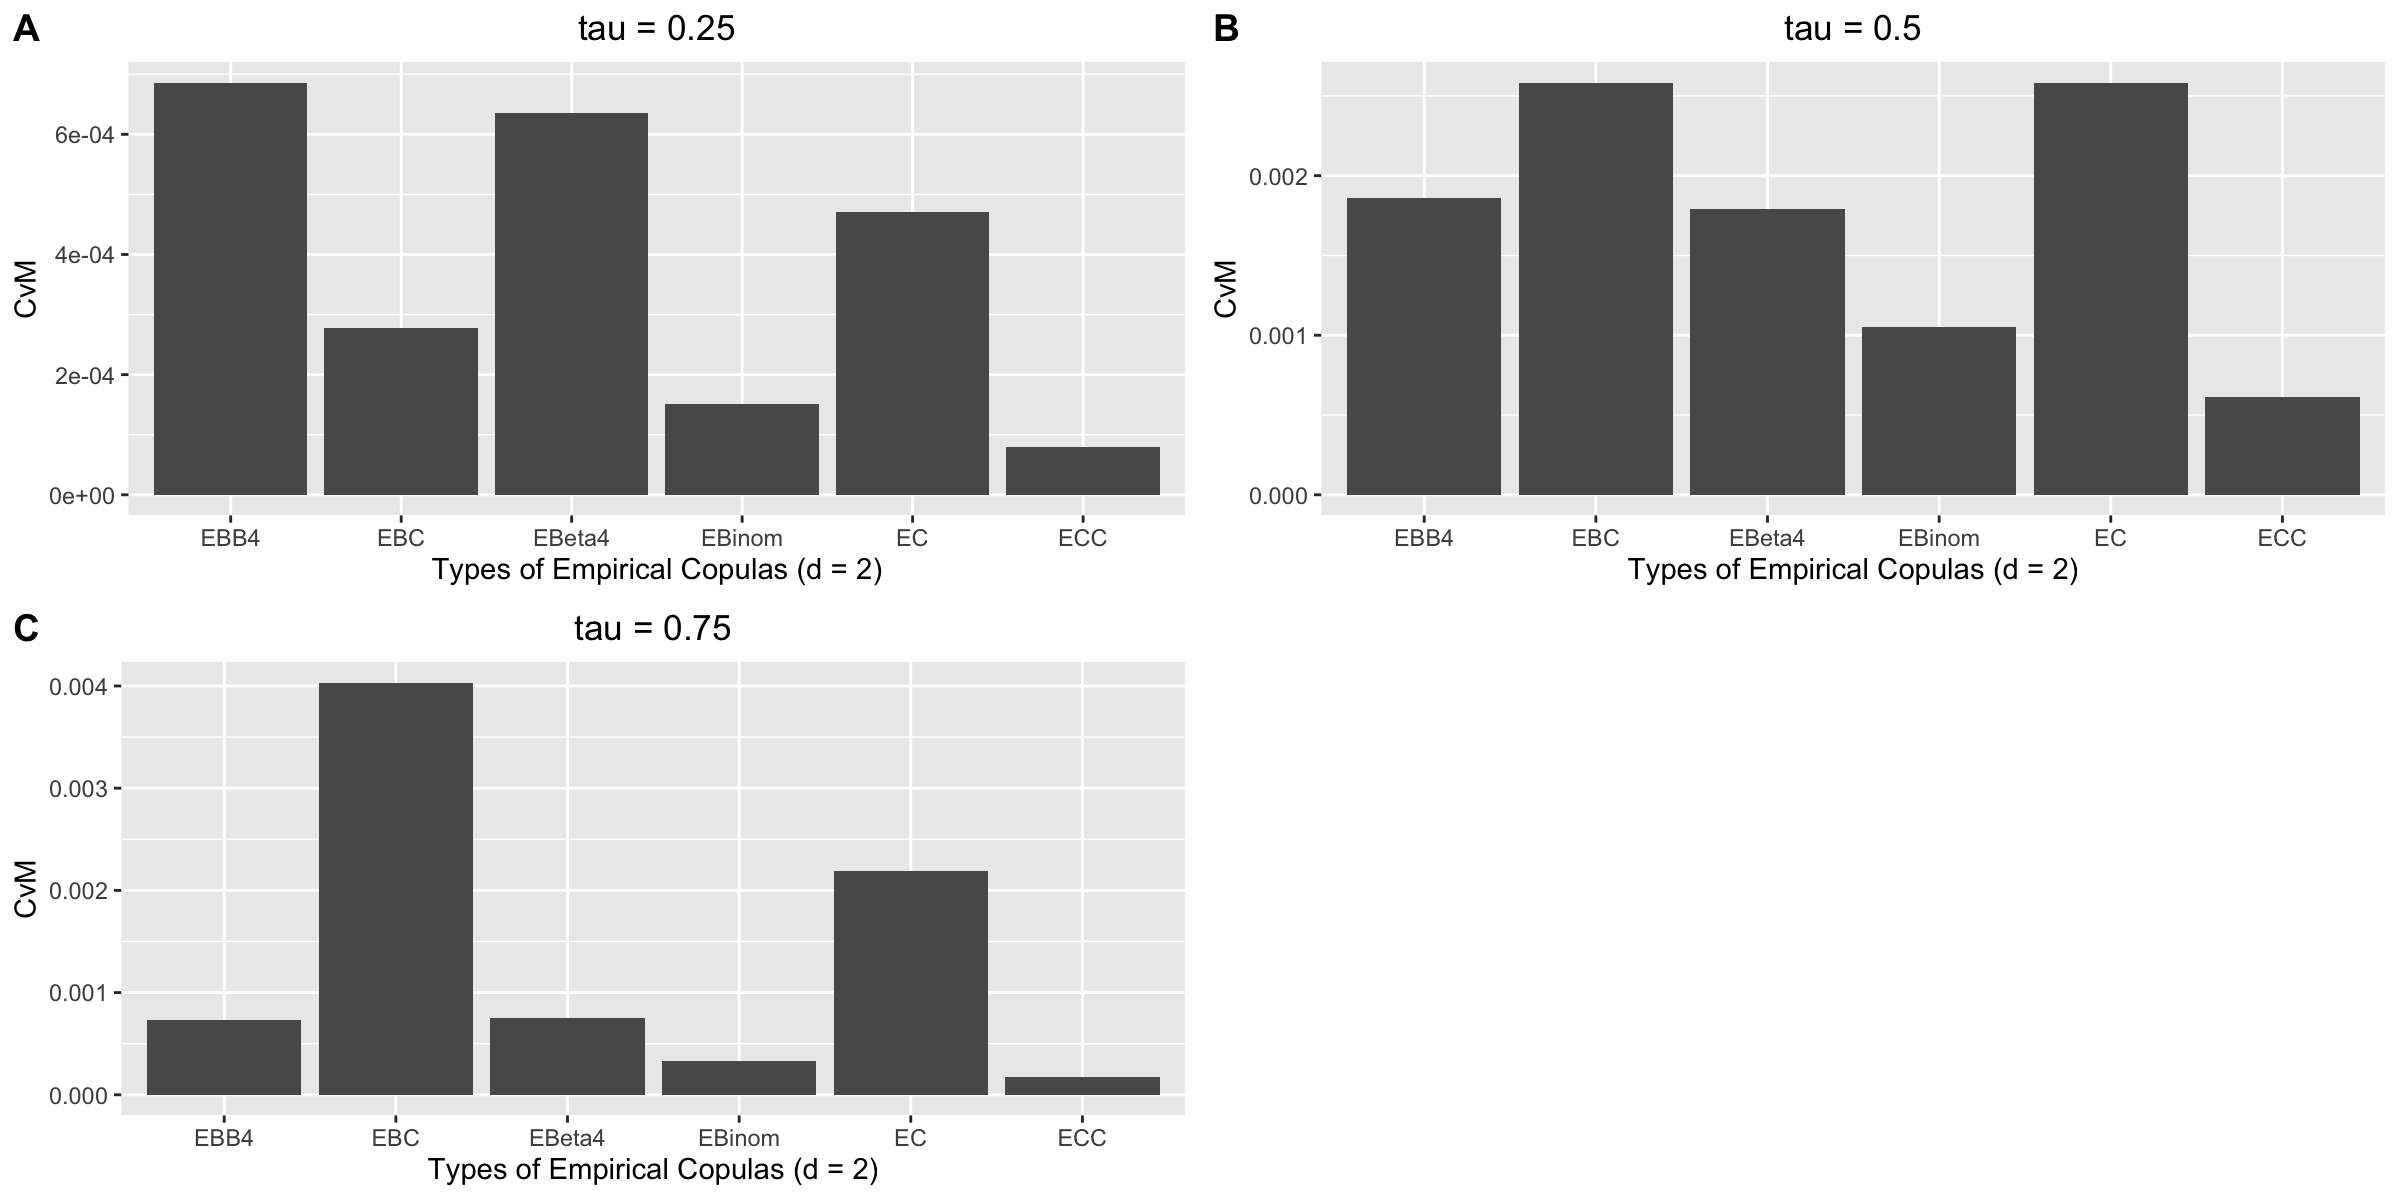
\includegraphics[width=17cm]{CumulativeCvM/C_2d_c_CvM.png}
\captionof{figure}{Clayton copula with $d$ = 2}
\end{center}%

\begin{center}
\label{C_3d_c_CvM}
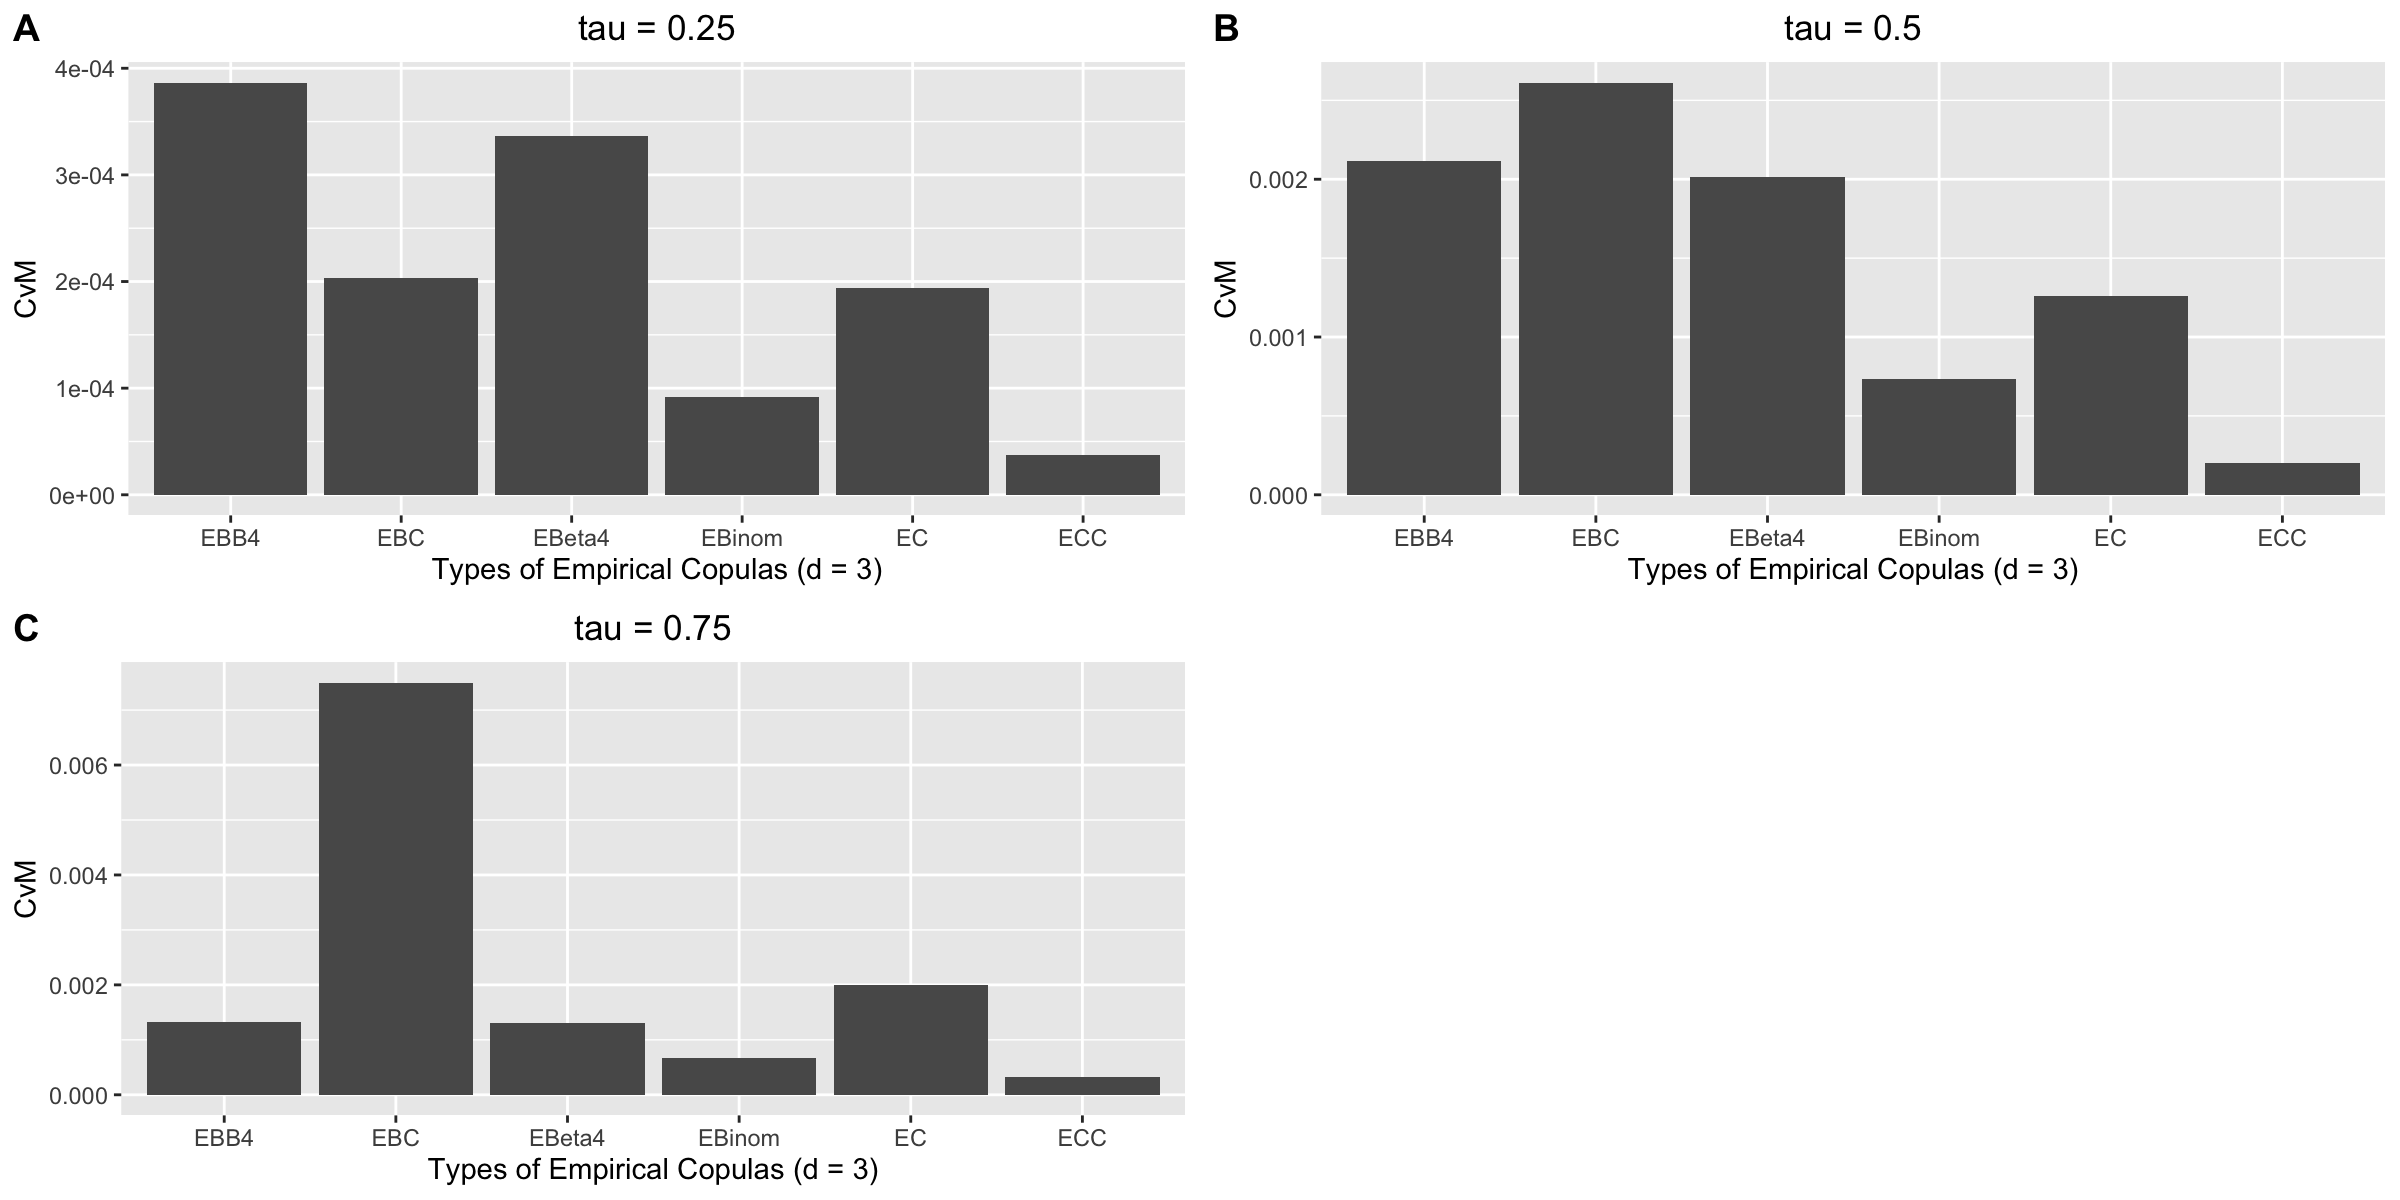
\includegraphics[width=17cm]{CumulativeCvM/C_3d_c_CvM.png}
\captionof{figure}{Clayton copula with $d$ = 3}
\end{center}%

\begin{center}
\label{C_4d_c_CvM}
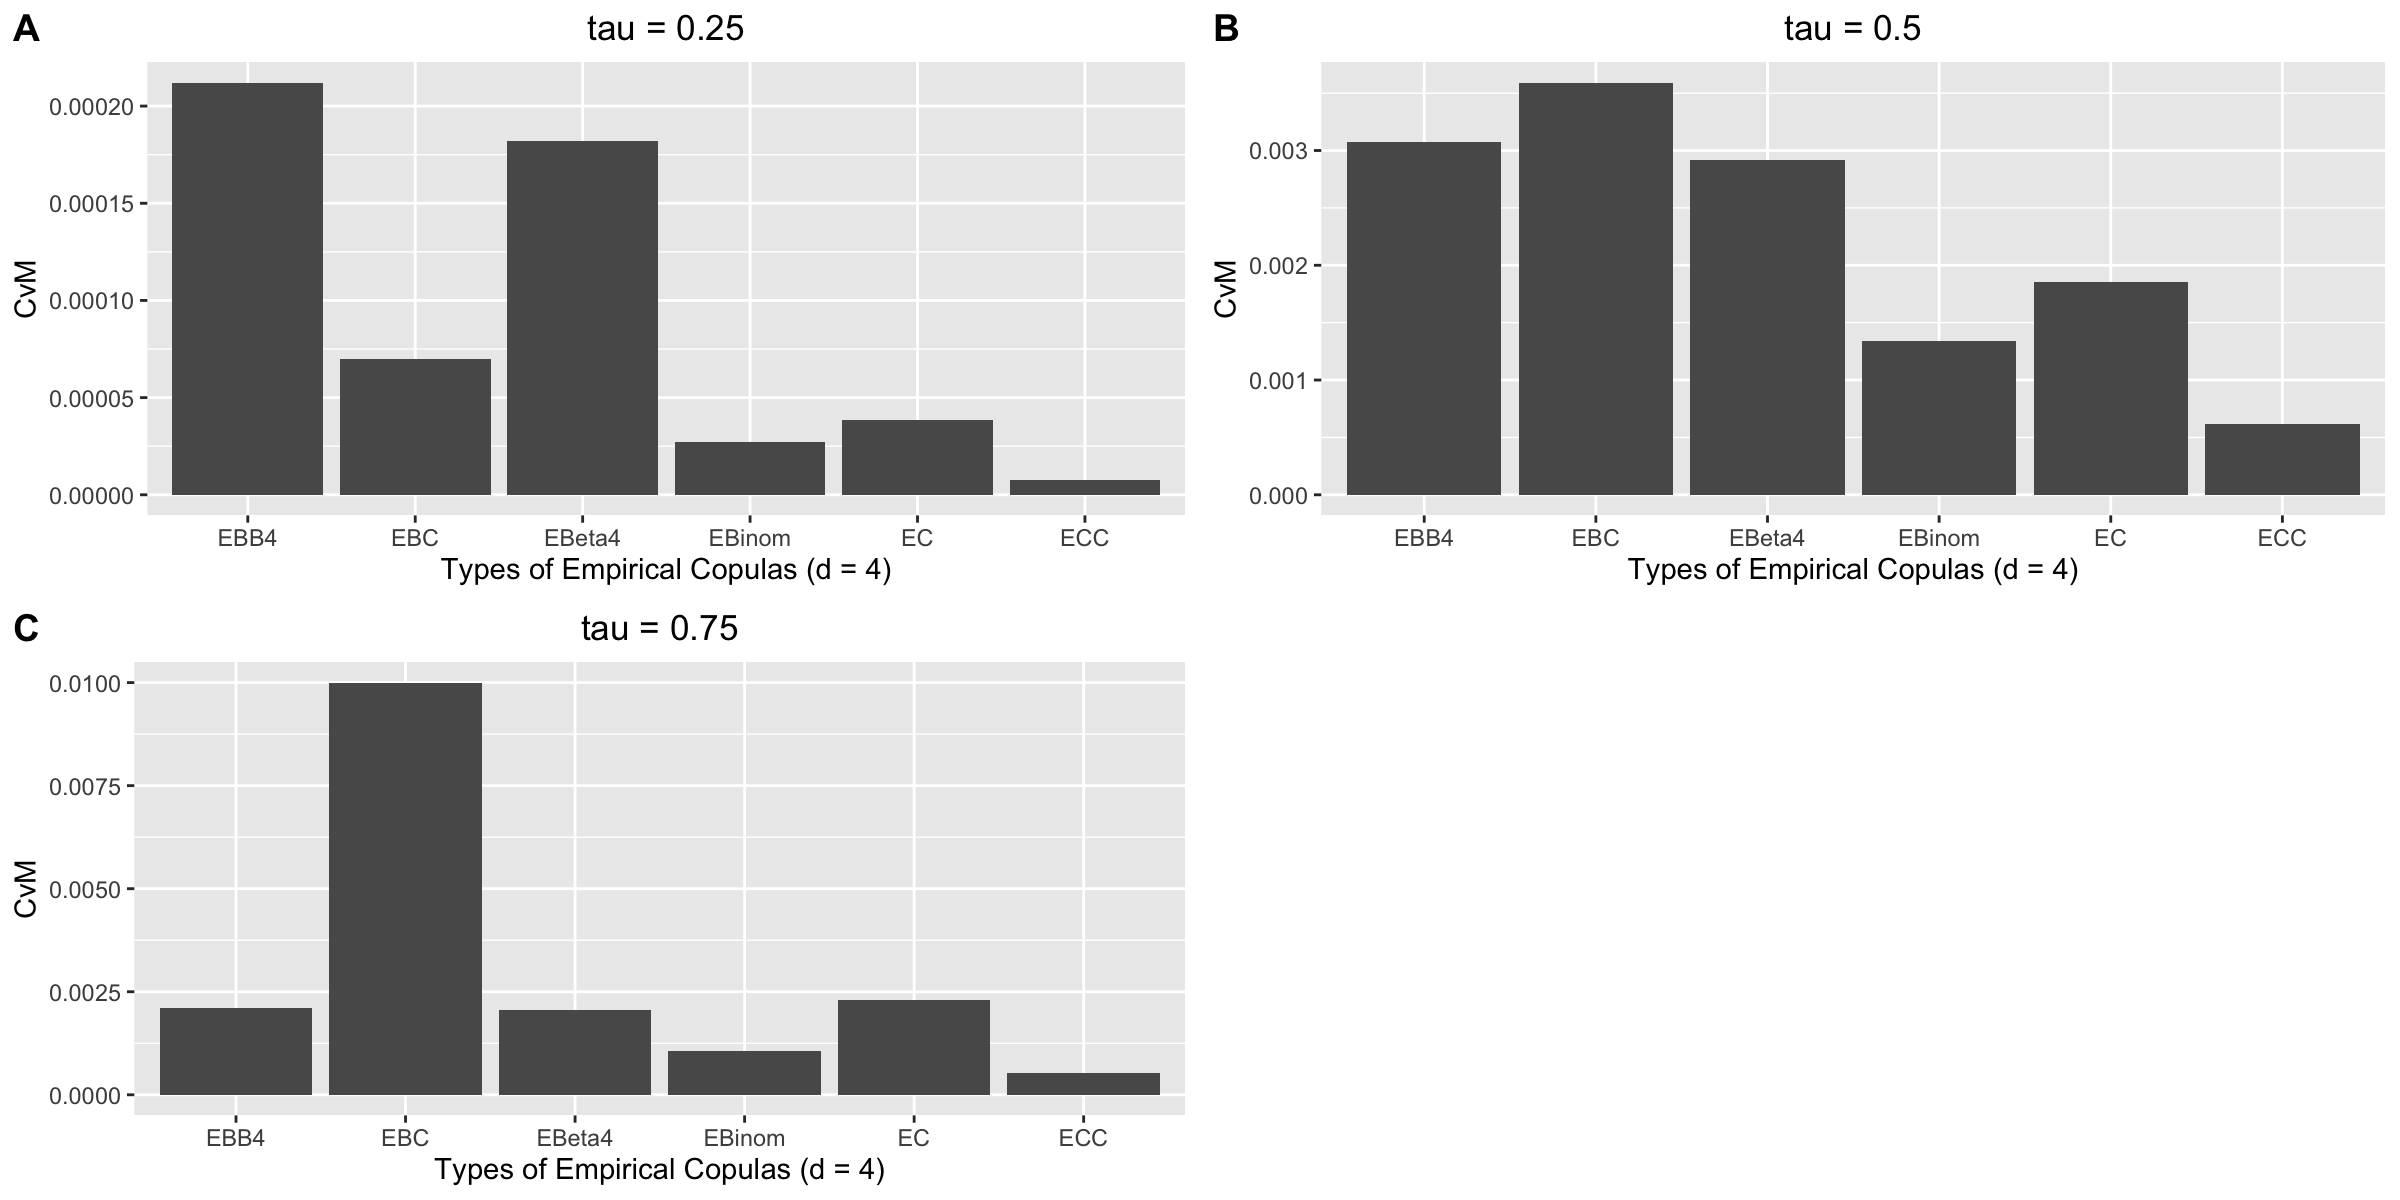
\includegraphics[width=17cm]{CumulativeCvM/C_4d_c_CvM.png}
\captionof{figure}{Clayton copula with $d$ = 4}
\end{center}%

\begin{center}
\label{C_5d_c_CvM}
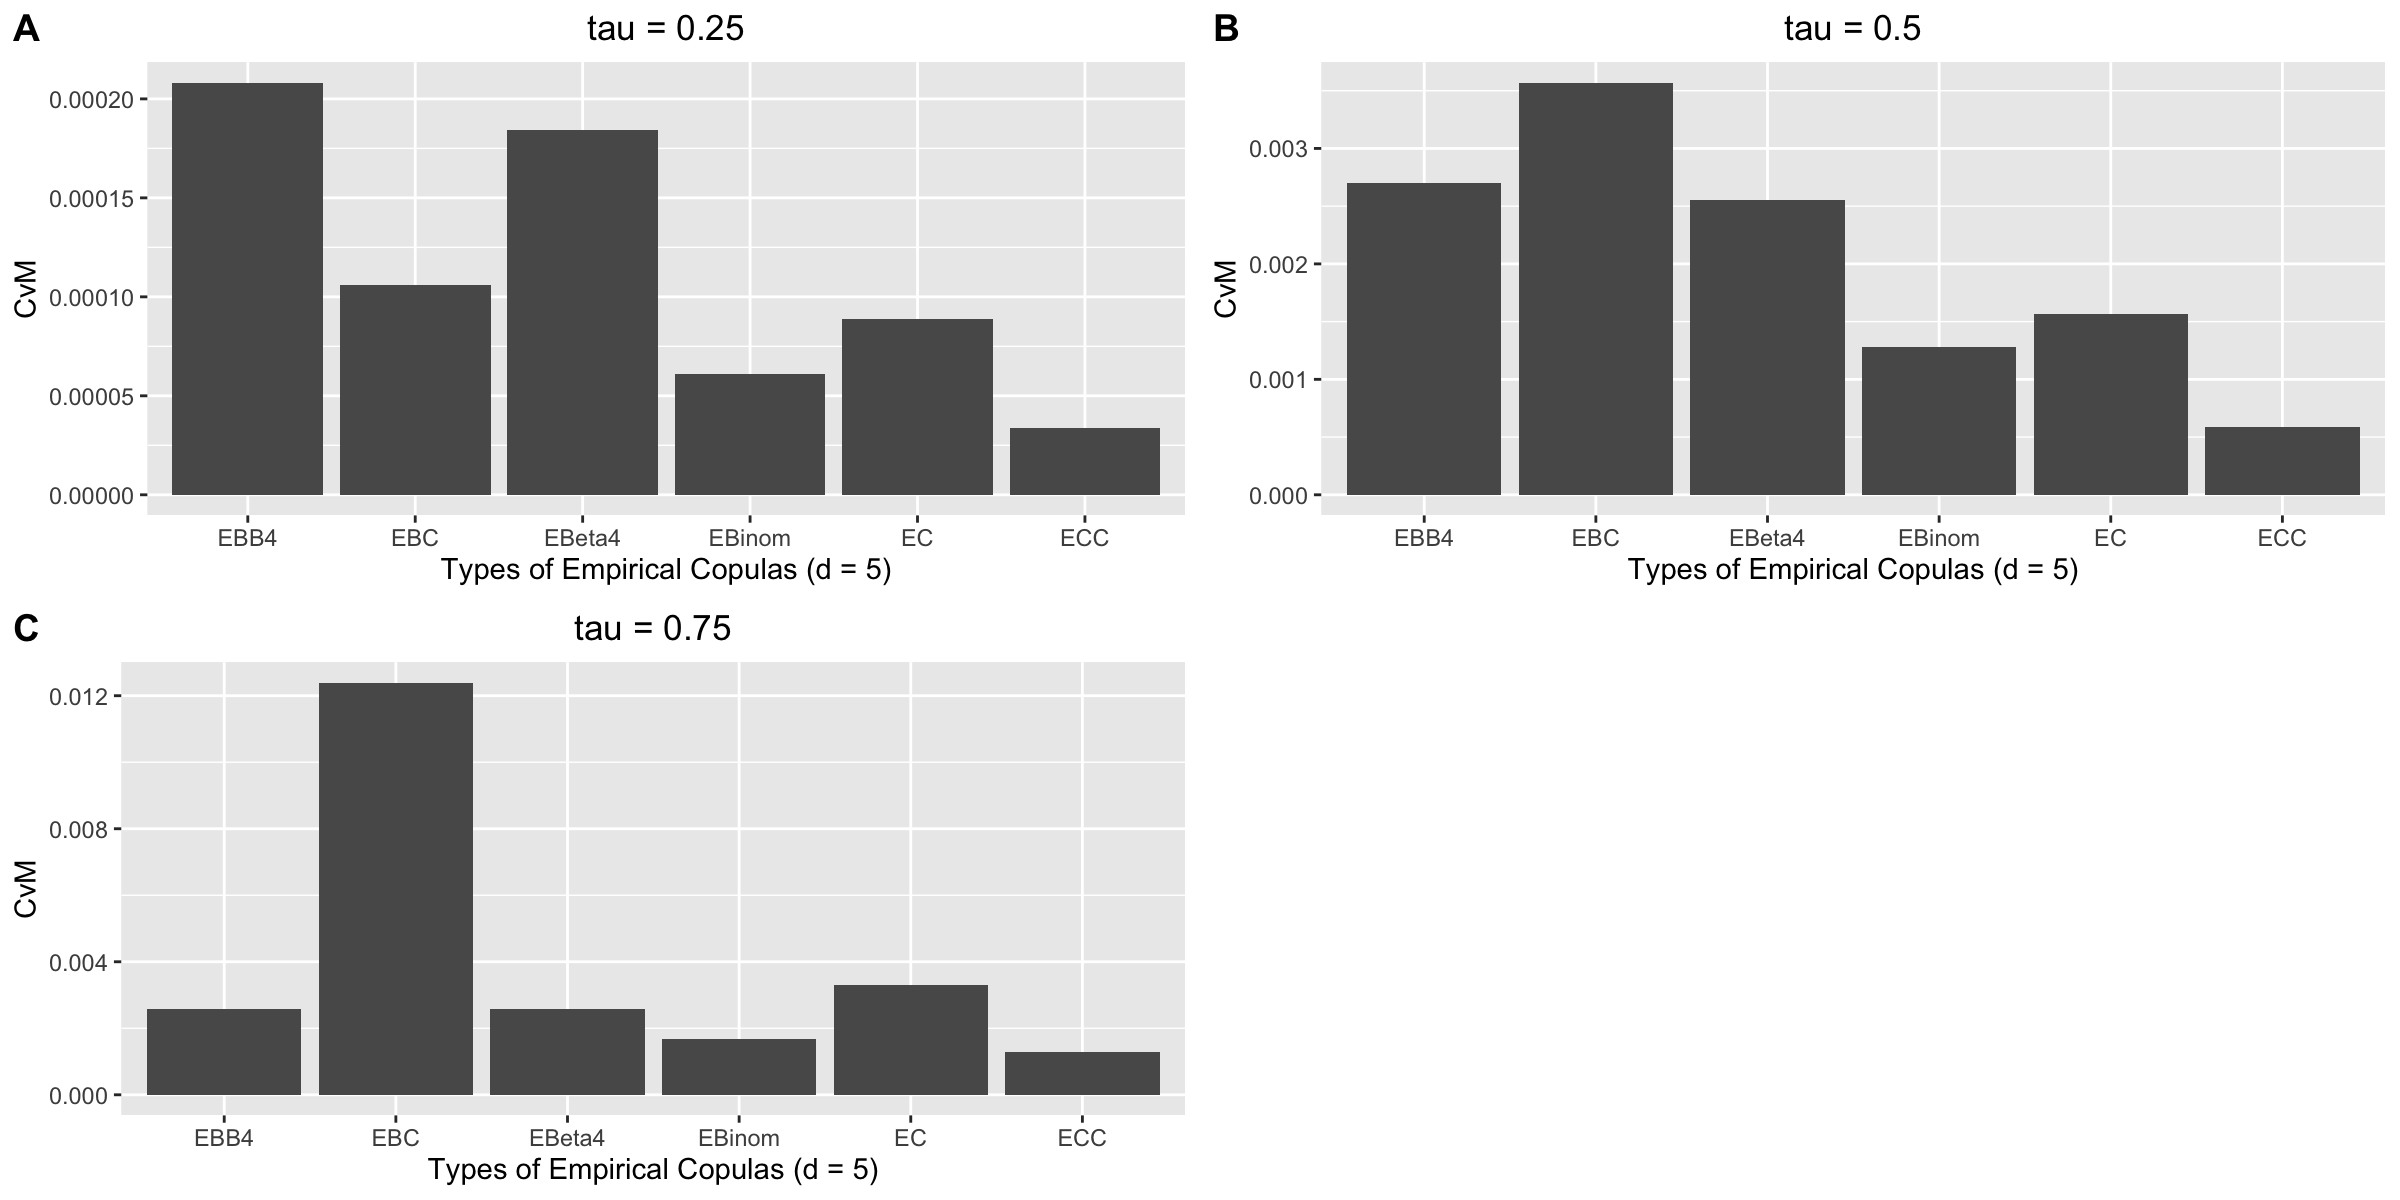
\includegraphics[width=17cm]{CumulativeCvM/C_5d_c_CvM.png}
\captionof{figure}{Clayton copula with $d$ = 5}
\end{center}%

\newpage
\subsection{Analysis: Cumulative probabilities}
Similar to the analysis for exceedance probabilities, there are a few conclusions that can be reached by analysing the aforementioned plots.\\
\subsubsection{Lower Kendall's tau values}
Similar to exceedance probabilities, the predictive performance of empirical copulas at the lower tail at low (negative) Kendall's tau values is poor. Similar to the intuition of the exceedance probabilities, a negative Kendall's tau represents that the points are concentrated on the top-left to bottom-right corner, and there is less probability mass in the bottom-left and top-right corner, for a bivariate case. Similarly, sampling with a sample size of $n = 125$ is unlikely to create any empirical mass at the lower-tail. For instance, by observing the plots corresponding to Student-$t$ copulas ($d = 2$ and $\tau$ = $\{ -0.75, -0.5 \}$) and Gaussian copulas ($d = 2$ and $\tau$ = $\{-0.75, -0.5, -0.25\}$) reflects that some empirical copulas have empirical mass 0 at the lower tail. As empirical copulas asymptotically (for large $n$) converge to the true copula, having a higher sample size can mitigate the failure to model the lower tail. However, as mentioned in the exceedance probability analysis, the availability of large amounts of joint data are often unrealistic.\\
\vspace{0.5cm}
It is to note that for Gaussian copulas ($d = 2$ and $\tau$ = $\{-0.75, -0.5\}$), it exhibits a rather peculiar sine-like / oscillating curve at the lower tail. This is caused as the cumulative probability is below the double precision / machine accuracy, which led to numerical errors or rounding errors in the R environment, as it is at negative order 17.
\subsubsection{Systematic underestimation of the lower-tail}
Similar to the exceedance probability, the estimators at higher values of Kendall's tau (usually positively valued) are extremely close to the true copula, but exhibit a systematic underestimation of the lower-tail probability. The reasoning of this observation is virtually identical to the exceedance probability counterpart. For brevity, the original empirical copula (which is not a copula due to its discrete uniform margins) place 0 empirical mass on $[0,\boldsymbol{u}]$ if all rows in $\boldsymbol{U}$ are larger than the evaluation point $\boldsymbol{u}$. Empirical copulas therefore systematically underestimate the true copula. \\
\subsubsection{Bias and variance of different empirical estimators}
From a bias standpoint, the best performing empirical copulas are the EBC-adapted empirical copula with binomial survival margins, and the empirical checkerboard copula. From the graph, it can be observed that the empirical checkerboard copula is extremely flexible around the true copula. A downside of this flexibility property is the high number of non-differentiable points relative to the other empirical estimators (except the empirical copula). On the other hand, the EBC-adapted empirical copula with binomial survival margins is differentiable nearly everywhere, yet retains the low bias with respect to the true copula, which slightly edges over empirical checkerboard copula despite its slightly inferior performance. The low bias for these two empirical copulas can also be observed via the CvM statistic plots (especially high Kendall's tau values). Notable exceptions include Student-$t$ and Gaussian copula with $d = 2$ and Kendall's $\tau = -0.25$, where both the EBC-adapted empirical copula with beta and beta-binomial survival margins strictly outperform the other empirical estimators. It is well-noted in the exceedance probability section that the EBC-adapted empirical copula with beta-binomial survival margins also outperforms its competition for Student-t and Gaussian copula with $d = 2$ and $\tau = -0.25$. On the other hand, the empirical copula and the empirical beta copula are the worst two performing estimators with respect to bias of the true copula, which is consistent with the exceedance probability section.\\
\vspace{0.5cm}
From a variance standpoint, the empirical checkerboard copula and empirical copula have the largest variance. It is intuitive as they are an interpolation of the empirical copula, and the discretized nature of empirical copulas leads to the high variance. The EBC-adapted empirical copula with beta-binomial and beta survival margins have the lowest variance.  \\
\vspace{0.5cm}
Similar to the exceedance probability modelling, no adequate estimators for extremely negative Kendall's tau are available due to the small sample size. It is only possible if the sample size is raised, which is limited by the restrictions mentioned earlier.

\newpage
\subsection{Recommendations}

In light of the analysis done for exceedance probabilities and cumulative probabilities at upper-tail and lower-tail respectively, we propose estimators that are best in replicating the true copula.

\subsubsection{Modelling exceedance probabilities at upper-tail}
$\tau \le -0.5$: N/A\\
$\tau = -0.25$: EBC-adapted empirical copula with beta-binomial survival margins \\
$\tau \ge 0$: EBC-adapted empirical copula with binomial survival margins

\subsubsection{Modelling cumulative probabilities at upper-tail}
$\tau \le -0.5$: N/A\\
$\tau = -0.25$: EBC-adapted empirical copula with beta or beta-binomial survival margins \\
$\tau \ge 0$: EBC-adapted empirical copula with binomial survival margins

\newpage
\section{Conclusion}
\vspace{0.5cm}
In this report, we have provided an overview of the important definitions and properties of copulas, introduced common copulas and rank correlation measures, and utilised 6 different types of empirical copulas. After that we have proposed algorithms to compute the exceedance probability and cumulative probability for a set of evaluation points (up-tail and low-tail respectively). Lastly, we plotted the exceedance probability and cumulative probability of the true copula and the empirical copulas proposed, and evaluated the underestimation and overestimation of the true copula by a goodness-of-fit test: Cramer-von-Mises test statistic.\\
\vspace{0.5cm}
Upon evaluation, we observe that despite the erratical behaviour of the EBC-adapted empirical copula with beta survival margins at negative Kendall's tau, it is the best estimator of the true copula for modelling cumulative probabilities at negative Kendall's tau together with the EBC-adapted empirical copula with beta-binomial survival margins. EBC-adapted empirical copula with beta-binomial survival margins is also the best performing estimator for modelling exceedance probabilities at negative Kendall's tau. For positive Kendall's tau, the EBC-adapted empirical copula with binomial survival margins is the best estimator for the true copula in modelling both cumulative and exceedance probabilities. This is in-line with the observations noted in \cite{KojadinovicYi2024Smooth}, where the MSE of the smoothed empirical copulas overperform the empirical copula, empirical beta copula and empirical checkerboard copula. Specifically, the empirical checkerboard copula's variance is too large despite its low bias.\\
\vspace{0.5cm}
To improve the procedure of modelling exceedance probabilities and cumulative probabilities, it is best to have a more efficient algorithm in computing the survival function of empirical copulas. For instance, the survival copula is calculated using Theorem \ref{SurvivalCopulaProperties}, which is extremely prohibitive as the dimension increases. The computation of survival function in dimension $d$ requires the computation of $2^{d}$ empirical copulas. Future research could look at how to derive the survival function of the empirical copula directly, instead of obtaining $2^{d}$ empirical copulas.\\
\vspace{0.5cm}
Moreover, this research is grounded on trying to recover the true copula, and we did not apply it into a real-life dataset (such as modelling joint default probabilities). Future research could entail providing a case study with a train-test split to evaluate the effectiveness of the class of empirical copulas outlined in this report. Recall that the financial crisis is inadvertently caused by a so-called ``misspecification" of the copula. To be more exact, the Gaussian copula is widely used in the pricing of complex financial products, but the event of joint defaulting is highly dependent, whereas the Gaussian copula is not, hence underestimating the probability of joint default causing huge financial firms to go under (such as the Lehman Brothers). Empirical copulas opened the door to a realm of possibilities due to the property that it will never be misspecified: empirical copulaS always converge to the true copula upon a high enough sample size. In this report, it is shown that at high Kendall's tau, empirical copulas closely resembles the true copula, hence showing its effectiveness potentially in financial modelling. It is though noted that the underestimation problem cannot be averted completely, hence it is recommended that further research can investigate suitable adjustment on the probability to minimize the difference between the estimator and the copula.\\
\vspace{0.5cm}
It is also remarked that, considering the small sample size, empirical copulas are rendered useless in the estimation of the exceedance and cumulative probability of the true copula under negative Kendall's tau, which is not ideal. In the real world, there are often indices that are negatively correlated / discordant. For example, fixed income securities thrive under a high interest rate environment, while equity stocks plummet due to the increased borrowing costs. If variables with negative Kendall's tau can be accurately modelled, it can allow more complex financial products / options to be created.\\
\vspace{0.5cm}
It could also have further applications in the insurance sector. Insurance products involving multiple-persons (couple insurance) is virtually unseen. Modelling bivariate mortality rates / morbidity rates (which is often extremely low) using the class of empirical copulas could also be one avenue of research.\\
\vspace{0.5cm}
All-in-all, Empirical copulas are extremely powerful and tractable under the correct assumptions due to their high flexibility and proximity to the true copula. By applying this technique to different settings, it can potentially revolutionise the financial sector, without revitalising past financial failures.



\end{flushleft}
 
\medskip

\printbibliography
\end{document}
